\documentclass[twoside,single]{lion-msc}

\title{Resolved spectroscopy of planet forming disks with SPHERE/IFS}
\author{Ardjan Sturm}

\affiliation{Huygens-Kamerlingh Onnes Laboratory, Leiden University}   % this is the default value
%\affiliation{Instituut-Lorentz, Leiden University}                     % for theoretical physics

%\affiliation{Huygens-Kamerlingh Onnes Laboratorium, Universiteit Leiden}   % experimental physics in Dutch
%\affiliation{Instituut-Lorentz, Universiteit Leiden}                       % theoretical physics in Dutch

\address{P.O. Box 9500, 2300 RA Leiden, The Netherlands}               % default address - uncomment if need be

%\newdate{date}{\day}{\month}{\year}           % definition of time and date using datetime package
%\newdate{date}{27}{08}{2010}
%\date{\displaydate{date}}

\studentid{S1663011}                           % check you student ID, LaTeX does not do this
\abstract{Here goes a wonderful abstract.}     % limit your self to 1/2 page or 500 words
\supervisor{Dr. M.A. Kenworthy}                         % Note that this should be a LION staff member!
\corrector{Prof. dr. J.M. van Ruitenbeek}                      % This could be a LION staff member or your external supervisor

%\degree{Master of Science}                     % The default option is "Bachelor of Science", change if needed

\major{Physics and Astronomy}                  % The default option is "Physics", change if needed
%\major{Physics and Mathematics}

% optional cover picture - should be jpg or pdf
\coverpicture{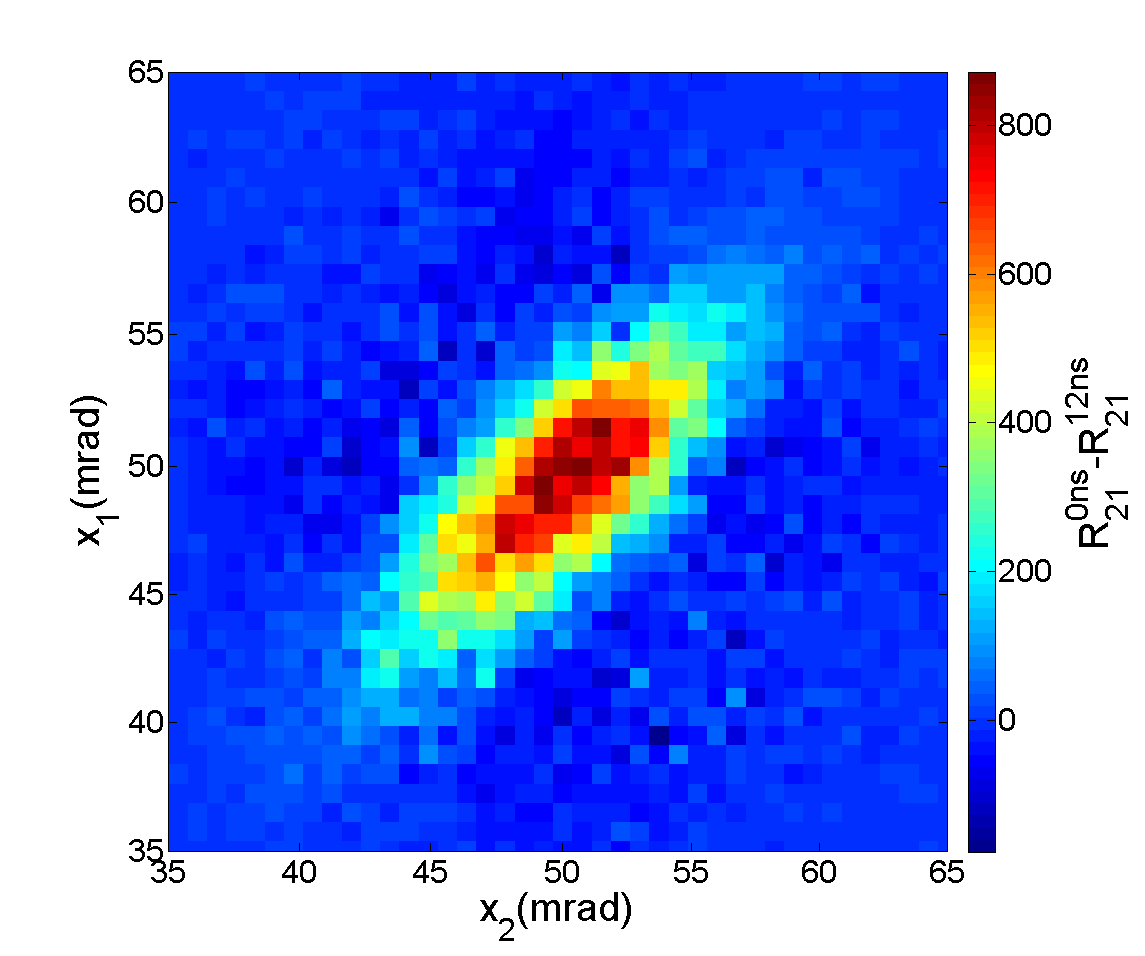
\includegraphics[width=7cm]{Fig3a.png}}

% Use this to make hyperlinks visible in the document.
% \hypersetup{colorlinks=true}

% ---------------------------------------------------------------- My definitions!
% \renewcommand{\vec}[1] {\ensuremath{ \overrightarrow{ #1 } }}
\renewcommand{\vec}[1] {\ensuremath{ \mathbf{ #1 } }}
% \bra \ket \braket and \proj
\newcommand{\bra}[1]{\ensuremath{\langle #1 \vert}}
\newcommand{\ket}[1]{\ensuremath{\vert #1 \rangle}}
\newcommand{\braket}[2]{\ensuremath{\langle #1 \vert #2 \rangle}}
\newcommand{\proj}[1]{\ensuremath{\vert #1 \rangle \langle #1 \vert}}

\newcommand{\kpar}{\ensuremath{k_\parallel}}
% ----------------------------------------------------------------

% \usepackage{tocloft}
% \renewcommand{\cftchapdotsep}{\cftdotsep}
\usepackage{subcaption}
\usepackage{makecell,tabularx}
\usepackage{longtable}
\usepackage{graphicx,wrapfig,lipsum}
\usepackage{caption}

\begin{document}

% roman numbering in the table of contents section
\pagenumbering{roman}

\maketitle

% Table of contents :  it is a good idea to include this into your thesis
\tableofcontents
\cleardoublepage

% The following list of figures and list of tables are optional. Remove the comments if needed
%\listoffigures
%\newpage

%\listoftables
%\newpage

% in the main part of the document use standard arabic numbers. Page counter resets to 1.
\pagenumbering{arabic}
\chapter{Introduction}
One of the biggest questions that arises in each human is how the world around us is formed. It intrigues children already that a pea grows to a complete plant and that their adults were once a child. Much research in astronomy is how the universe has taken his shape as it has today. How stars, planets and galaxies are formed. A long time it was a question if the solar system was the only place in the universe to harbor planets. Since then, many indirect methods were developed that could tell if a star hosted planets and the first exoplanet was soon confirmed.
\bigskip

Scientists have made huge progress in the last few decades in understanding the formation of stars and planets. It is now common known that stars are formed by the collapse of a big cloud of gas and dust. The gas and dust that is left in the cloud after the birth of a star starts to fall towards it. This accretion material starts to orbit the star in a plane due to the conservation of angular momentum, forming an accretion disk. In this accretion disks, planets start to form, when grains form pebbles, pebbles planeto\"ids and planeto\"ids planets. 
\bigskip

The formation of these planets is actually much more complex since there are many processes going on in a disk. Direct imaging of planets and disks has been impossible for a long time, since the contrast between stars and planets is too big and the point spread function (PSF) of the star too much extended. With the development of special optics called coronographs that improve the contrast, special adaptive optics that correct for the distortion of the light in the atmosphere and special techniques to reduce the stellar PSF, we are now able to image planets and protoplanetary disks directly. This provides us detailed information of the conditions in different planetary systems and protoplanetary disk, which improves our understanding of the formation of planetary systems.
\bigskip

SPHERE, one of the instruments of the Very Large Telescopes (VLT) in Chili, was build for direct imaging of planets. This instrument collects high resolution data of exoplanets and circumstellar disk. One mode of the subsystems of the instrument gives both light to IRDIS and IFS. IRDIS is the InfraRed Dual Imaging and Spectograph subsystem that provides classical imaging, dual band imaging, dual-polarization imaging and long slit spectroscopy with a good resolving power, IFS is the Integral Field Spectroscope that provides a data cube of 39 monochromatic images. \cite{Observatory2007} Since IRDIS data is easier to reduce and to analyze, and the field of view (FOV) of IRDIS is much bigger than the FOV of the IFS, IRDIS data is much more often analyzed than IFS data. Since there exists as much IFS data as there exists IRDIS data, much of the disk data made by IFS is still unpublished.
\bigskip

Since the IFS can provide a resolved spectrum of an object, it is possible to get a spectrum of a protoplanetary disk. Untill now, we do not have detailed information about the colour of the object that mainly will be analyzed in this project, the disk around T-Tauri star RX J1615.3-3255 (RX J1615). Reliable spectral information of protoplanetary disks can lead us in the future to a better understanding of ongoing planet formation in protoplanatary disks in general, since resolved spectral data of a disk can tell us something about the grain properties in different regions of the disk. This could provide us a better feeling of the requirements for a planet to form in protoplanetary disks. 
\bigskip

There are many steps to make for this to achieve. One of the first steps is a good reduction of the raw data. One of the main goals of this research is hence to investigate what the best way is to reduce the raw data, what calibration data is needed and which calibration steps there have to be taken. There are various effects at play that we want to understand if we have this basic reduction done. It appears that the disk gets better detected at longer wavelengths. One of the goals of the project is to check if this is a property of disks, or that this is only an effect of the adaptive optic performance getting better at longer wavelengths, which it generally does. By use of different post-processing techniques the starlight can be subtracted in order to detect the disk, but these techniques can effect the spectrum and the morphology of the disk. One goal of the project is to check how strong these effects are and what we can trust out of the data.
\bigskip

\chapter{Theory}
\section{protostars}
HD 97048 is a Herbig Ae/Be star, which means that it is a young 2-3 Myr, \cite{VanDenAncker1998}, pre-main-sequence star embedded in an envelope of both gas and dust. This type of star is in the fase of gravitational collapse towards a star and has hence no hydrogen burning in their center, what would stop the gravitational collapse. Herbig stars are divided into two groups, often called group I and group II. Group I stars have been interpreted as stars that host a brigth circumstellar disk with a large gas component. Group II stars are assumed host a much less flared protoplanetary disk, which means that the light of the star cannot reflect on the surface of the disk anymore. This means that the disk only emits light at his own temperature, which means that this type of disks are much less prominent in available data.
\bigskip 

HD 97048 has a spectral energy distribution which is classified as a group II Herbig Ae/Be star. It is well known that this star has a large circumstellar disk, which has a radius over 600 au \cite{Doering2007}. There are four different rings resolved at $46.4\pm 4.7$au, $161\pm 17$au,	$274\pm 28$au and $341\pm 35$au \cite{Ginski2016}.

\section{The object}
The main object of study is HD 97048. This star belongs to the constellation Chamaeleon and has co\"ordinates 11 08 03.3106 -77 39 17.490. The distance to HD 97048 is $158^{+16}_{-14}$  \cite{VanLeeuwen2007} and the mass of the star is estimated to be $2.5\pm 0.2 M\odot$ \cite{VanDenAncker1998}. The spectral type of HD 97048 is A0Vep. A0 means that the star has an effective temperature of 10,000 K \cite{Maaskant2013}. Vep means that it belongs to the class of the main-sequence stars or dwarfs, but also that it is a star with unspecified peculiarity and emission lines present.
\bigskip

\chapter{Instrumentation}
\section{SPHERE}
\begin{figure}[hb]
\centering
\begin{subfigure}{.6\textwidth}
  \centering
  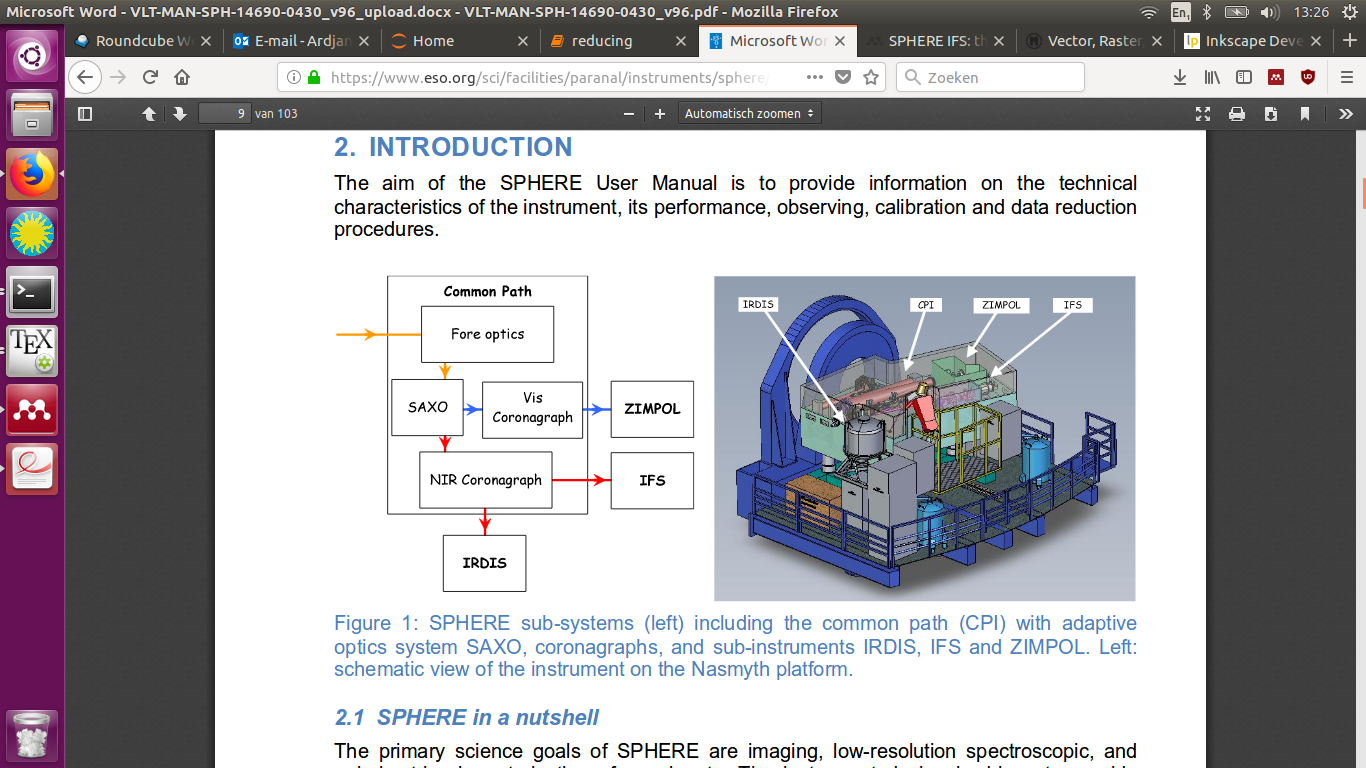
\includegraphics[trim={25cm 6cm 7cm 8.8cm},clip,width = 1\linewidth]{overviewSPHERE}
  \caption{\citep{Observatory2007}}
  %\label{fig:sub1}
\end{subfigure}%
\begin{subfigure}{.4\textwidth}
  \centering
  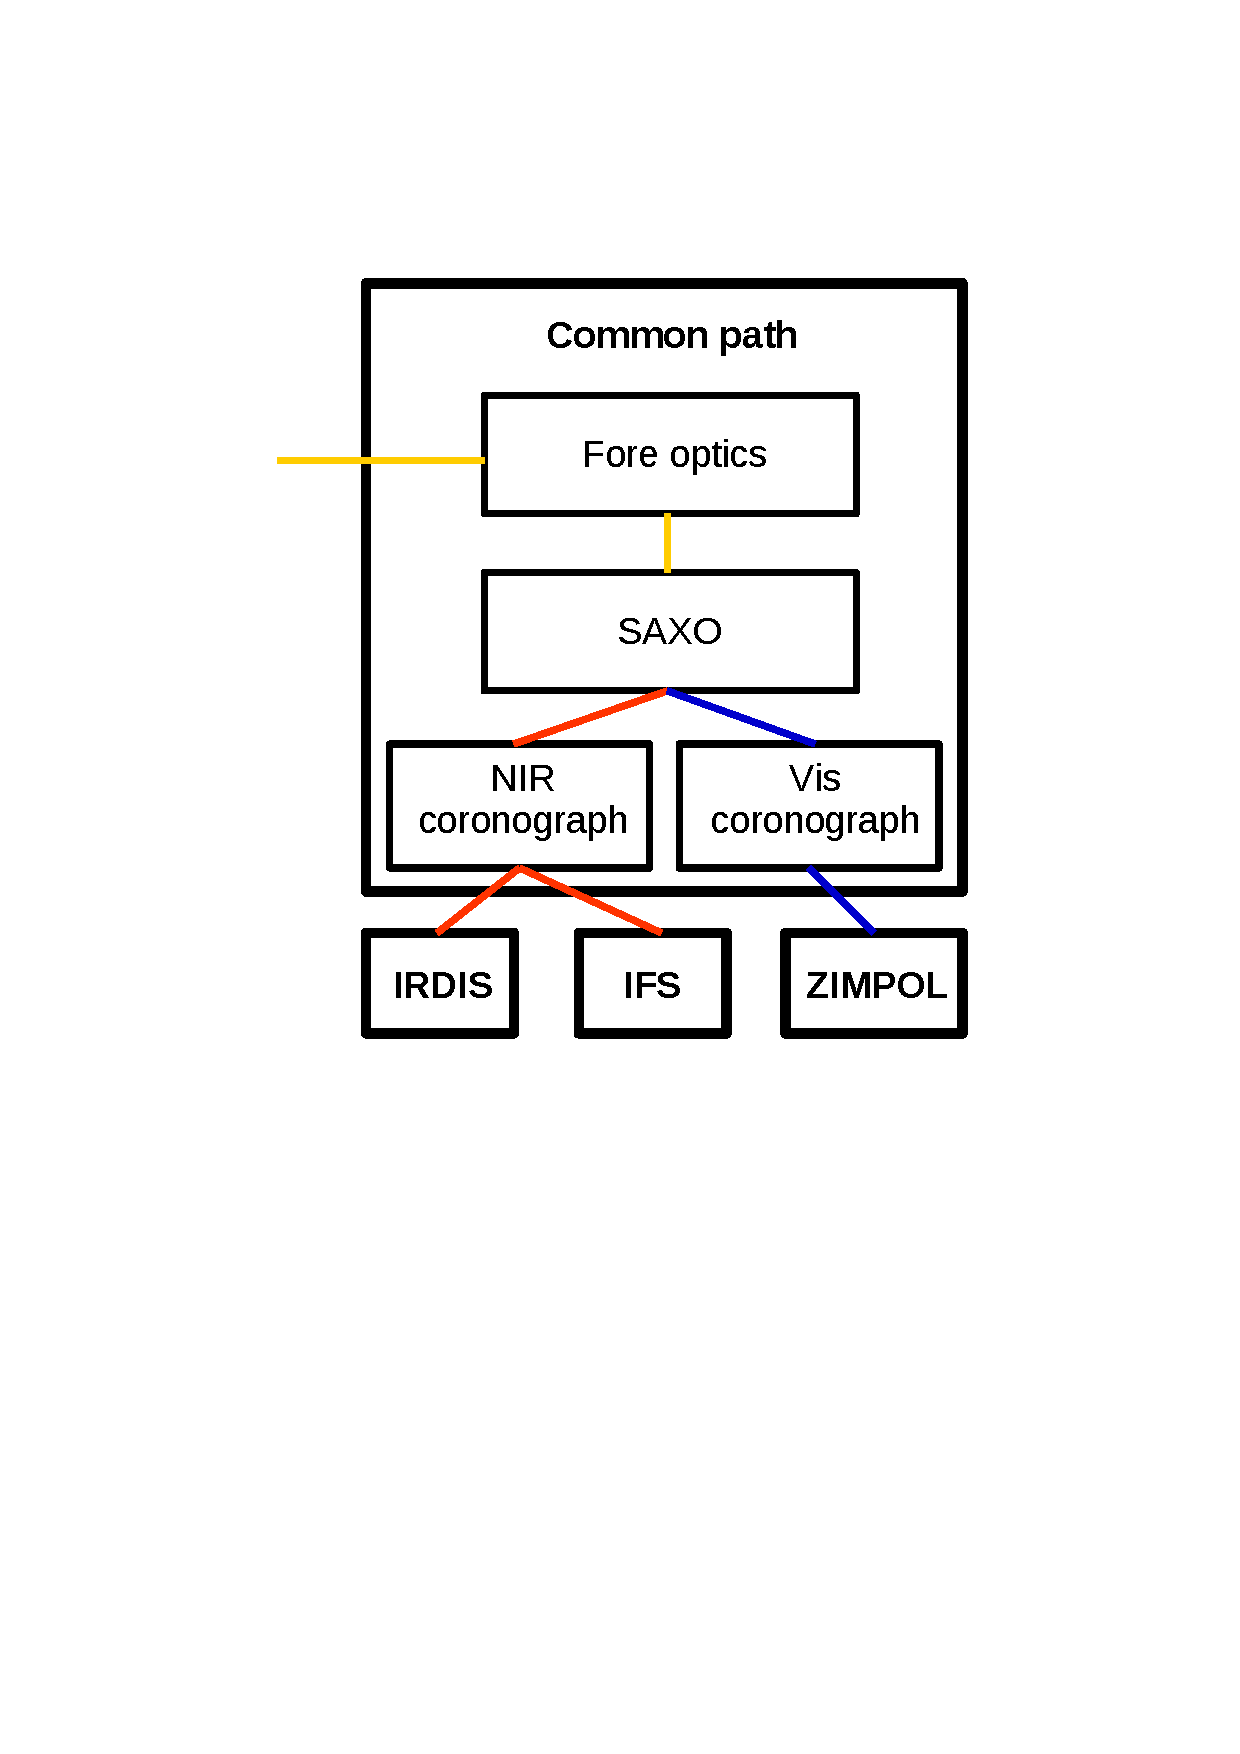
\includegraphics[trim={5cm 12cm 3.5cm 3.5cm},clip,width=1\linewidth]{overview_SPHERE}
  \caption{}
  %\label{fig:sub2}
\end{subfigure}
\caption{overview of SPHERE}
\label{fig:overviewSPHERE}
\end{figure}

SPHERE, (Spectro-Polarimetric High-contrast Exoplanets REsearch) is an instrument for the VLT which is optimized for high contrast imaging. The instrument is placed in the Nasmyth room of one of the VLT units, as shown in Figure \ref{fig:overviewSPHERE}. The instrument can be split up into four systems, the common path optics and three subsystems, IRDIS, IFS and ZIMPOL. Zimpol uses visible light and IRDIS and IFS both near infrared light (NIR). Since IRDIS and IFS can work at the same time, by guiding a part of the spectrum to the IFS and a part to IRDIS by use of a dichroic, we will discuss IRDIS briefly and take some time to look at the IFS in detail.

\subsection{Common path}
The common path interferometer (CPI) is the main system of SPHERE that powers all the cryostats and motors, corrects the light for many distorsions and connects all the sub-systems to the light path. The common path can also include coronographs in the light path. 

\subsubsection{pupil stabilizing fore optics}
SPHERE has a derotater that is able to stabilize the field or the pupil on the detector. This stabilization is needed because of the rotation of the earth around its axis. This rotation of the earth causes a rotation of the field due to a change in parallactic angle and altitude of the object and a rotation of the pupil that is only due to the change in altitude of the object that is observed. This derotator can also switched of in order to take data which can be used in angular differential imaging routines. The pupil has an offset with respect to the true north of -135.99$^o$, which means that all the data taken with SPHERE has to be rotated with that angle in order to make sure that north is pointing up in the data. The field of view of the IFS is for technical reasons rotated with respect to the IRDIS field of view by 100.48$\pm$0.10$^o$. IFS has an aditional derotator to align the north up. But if the derotators are turned off in observations, which was the case in our data, providing a possibility to do angular differential imaging, the data has to be rotated with the offset in order to make sure that the north is pointing up. %###\cite{maire} 
\bigskip

After entering the instrument, the light path is protected against many possible noise sources. The vibrations in the Nasmyth platform that are caused by seismic activity or other reasons are damped by use of servo-controlled pods and the whole instrument is protected against changes in temperature and dust by a protective cover. The light is then propagated in the complete spectral range from 0.450$\mu m$ to 2.320$\mu m$ to the beamsplitter that splits the light in a visible part for ZIMPOL, the polarimetric subsystem that works in the visual range and a near infrared (NIR) part for both IRDIS and IFS. If ZIMPOL is not used, all that light goes to the wavefront sensor that is used by the adaptive optics system to correct for the aberations of the light in the atmosphere. After the dichroic, the light is guided through an atmospheric dispersion corrector (ADC) that corrects for dispersion effects in the atmosphere, due to changes increase in altitude of the object.
\bigskip

\subsubsection{adaptive optics}
Sphere AO for eXoplanet Observation (SAXO) is the adaptive optics module of SPHERE. It is composed out of different components, each correcting a part of the distortion of the light. The bundled information fo these components is send to the deformable mirror (DM), that corrects for phase perturbations of up to a frequency of 1.2 kHz by use of the 41x41 actuators that are able to deform the mirror \citep{Observatory2007}. The phase perturbations are measured by different components.
\bigskip

\begin{figure}[htbp]
\centering
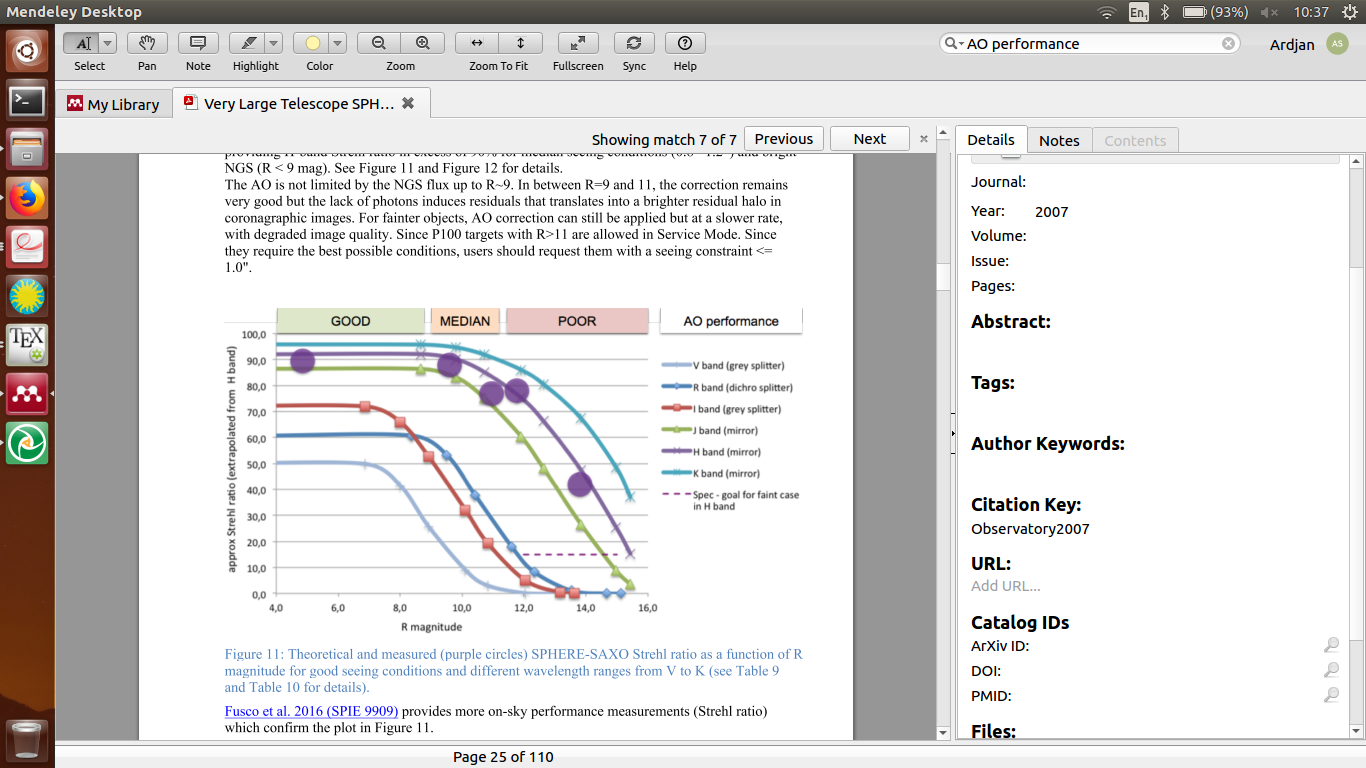
\includegraphics[trim={7cm 4.5cm 19cm 10cm},clip,width = 1\textwidth]{aoperformance}
\caption{Theoretical and measured (purple circles) SPHERE-SAXO Strehl ratio as a function of R magnitude for good seeing conditions and different wavelength ranges from V to K\citep{Observatory2007}}
\label{fig:aoperformance}
\end{figure}

The turbulence is measured by a wavefront sensor that transposes the phase shift to an intensity distribution on a detector. The wavefront sensor that is used is a 40x40 lenslet Shack-Hartmann sensor. (ANUGU!!!!) This sensor uses a lenslet array that produces a spot on a detector for each lenslet. A distorted incomming wavefront changes the position of the focal spot of a lenslet on the sensor. From these positions the local tilt of the wavefront can be calculated. Other distorsions such as image motion, pupil shift and distorsion in the instrument are measured with tip tilt sensors and corrected by the DM, correcting the only the large scale differences that these distorsions cause.
\bigskip

The wavefront of the object that is incomming, is accurately corrected in a radius of about 20 $\lambda/D$ in the image plane. Further out is the PSF still corrected, but not enough to suppress the stellar halo. The correction of the AO is dependent of the R magnitude, since the Shack-Hartmann sensor measures the perturbations of the wavefront in the range of the R filter. The more light is provided to the sensor, the more accurate the distorsions of the wavefront can be measured \ref{fig:aoperformance}, which could drastically change the overall performance of the AO and hence the quality of the data.

\subsubsection{coronographs}
A coronagraph is a device that increases the contrast between the star in the central and the background by surpressing the PSF that is produced by the star. SPHERE has several coronagraphs for different conditions the instrument can work. All coronagraphs consist of three components. At the begin of the light path an apodizer changes the beam profile and improves the dynamic range of the image that way. Further downstream focal plane masks shift the phase of the image in one of the foci of the instrument, creating a self-destructive interference that blocks most of the light of the star.  Behind the focal plane mask a Lyot pupil stop reduces the flare in te system, meaning that reflected and scattered light on the different optical components is left out of the image. Different combinations of these three elements have different results on the final image and all the combinations have conditions they work the best. Think of the wavelength range at that moment is used, seeing and needed inner working angle.

\subsection{IRDIS}
IRDIS is the InfraRed Dual Imaging and Spectograph subsystem that works in the NIR. IRDIS has a field of view of 11" x 12.5" and has several modes in which data can be acquired. IRDIS provides classical imaging, dual band imaging, dual-polarization imaging with the filters Y to Ks and long slit spectroscopy if it used alone. There are also two modes wherein IFS and IRDIS take data in parallel. This can be achieved by the use of dichroic filters that let light in a certain wavelength range pass and reflects the other light. If the instrument is set up in IRDIFS mode, the IFS gets all the light in the Y-J band and IRDIS is able to do narrow band or broad-band H Dual band imaging in parallel. In the IRDIFS\_EXT mode, the IFS get the light in the range from Y band to H band, leaving IRDIS with the possibility to get dual band imaging data with lower efficiency in a narrow-band filter or in broad-band K. The end-to-end efficiency of both possibilities are shown in Figure \ref{fig:systemthrougput}. 

\begin{figure}[htbp]
\centering
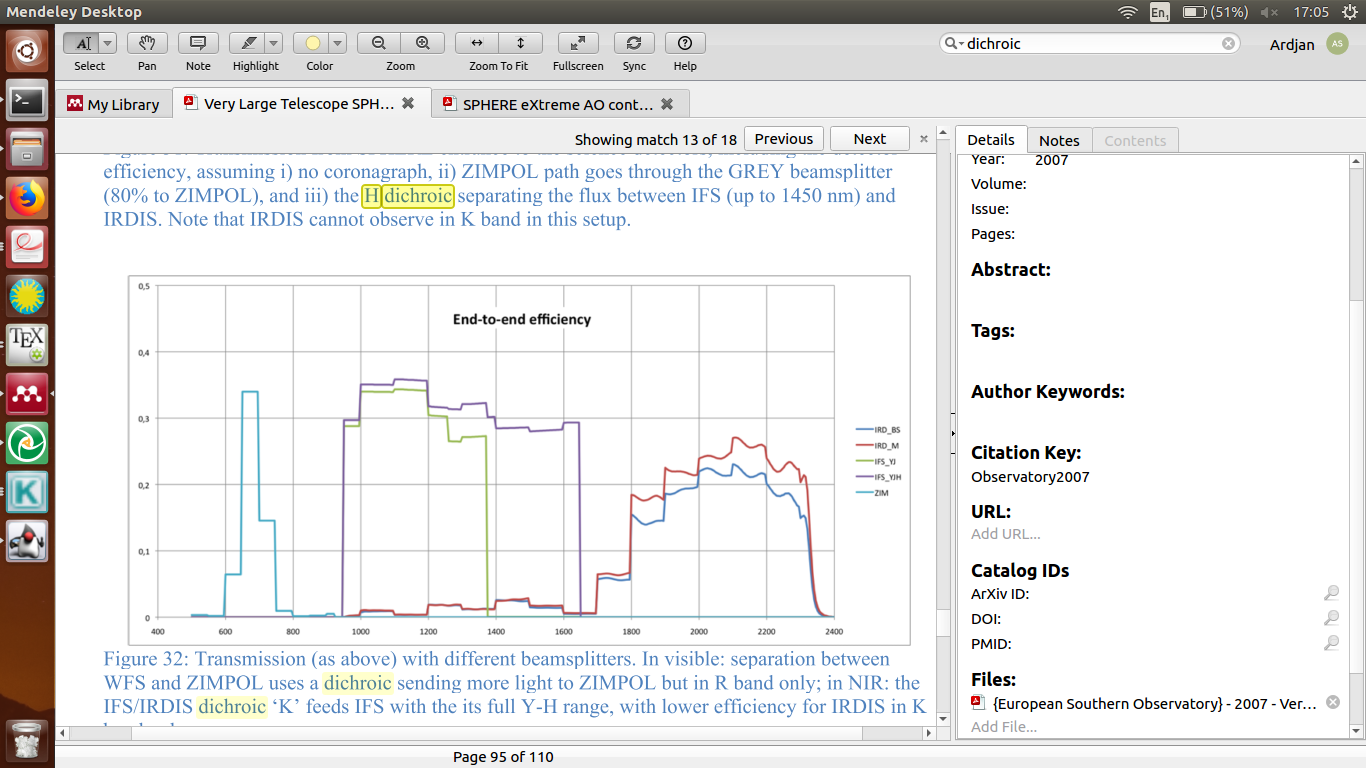
\includegraphics[trim={4cm 4.3cm 16cm 9cm},clip,width = \textwidth]{systemthroughput}
\caption{End-to-end efficiency if both IFS and IRDIS get light. The light of ZIMPOL is in this case for the AO system.}
\label{fig:systemthrougput}
\end{figure}

\section{Integral Field Spectroscope}
\begin{figure}[htbp]
\centering 
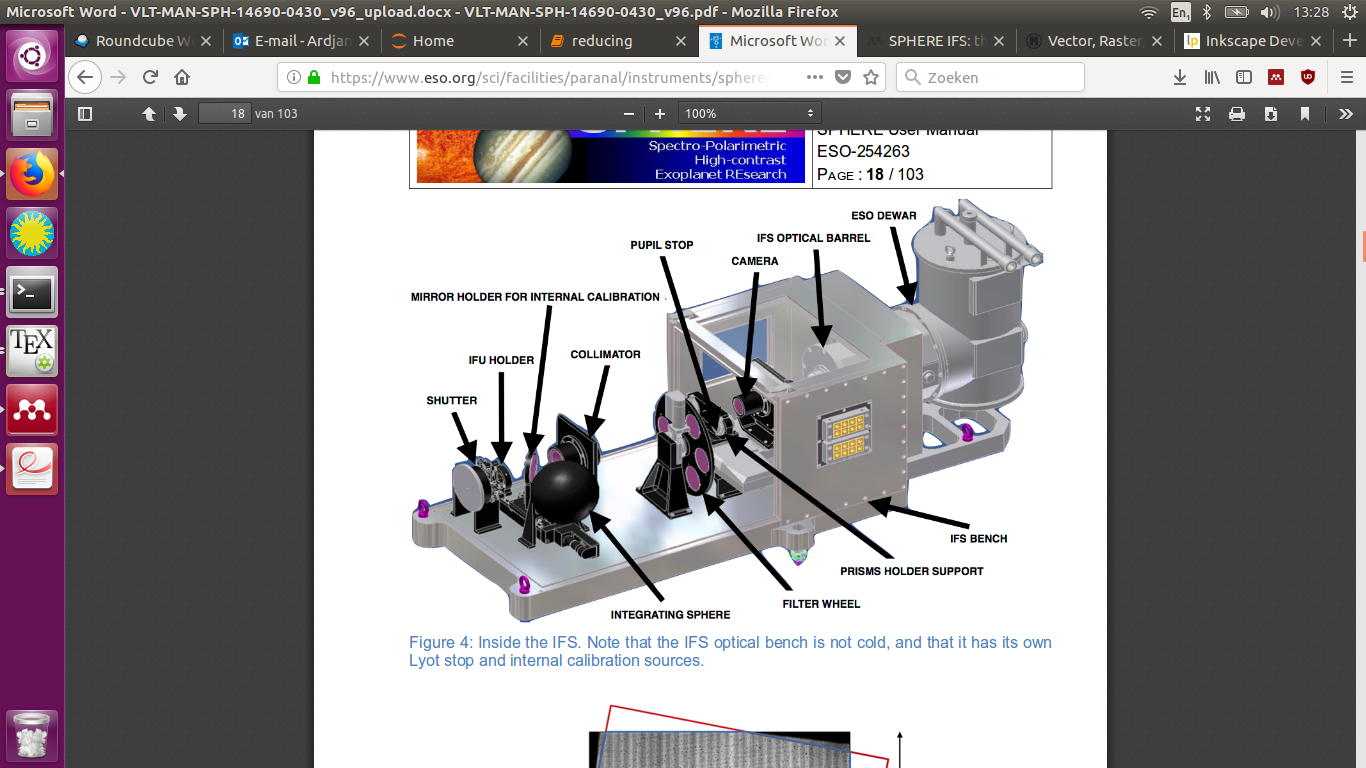
\includegraphics[trim={13cm 5cm 10cm 7cm},clip,width = 0.6\textwidth]{overviewIFS}
\caption{Overview of the IFS\cite{Observatory2007}} 
\label{}
\end{figure}

The integral field spectroscope is a subsystem of SPHERE that is able to collect data over a wavelength range from 0.95 $\mu m$ up to 1.346 $\mu m$ or 1.677 $\mu m$, depending on the mode (Y-J or Y-H) the instrument is in. The IFS receives stable light, which is corrected for many distorsions in the common path and at the deformable mirror. The IFS has a total field of view of 1.73" x 1.73", so much smaller than IRDIS', but enough to be able to detect inner structures of protoplanetary disks. IFS focuses on the NIR because that is the range in which the most useful broad molecular bands of the planets are expected to show off.

\subsection{IFU unit}
\begin{wrapfigure}{R}{0.6\textwidth}
\centering 
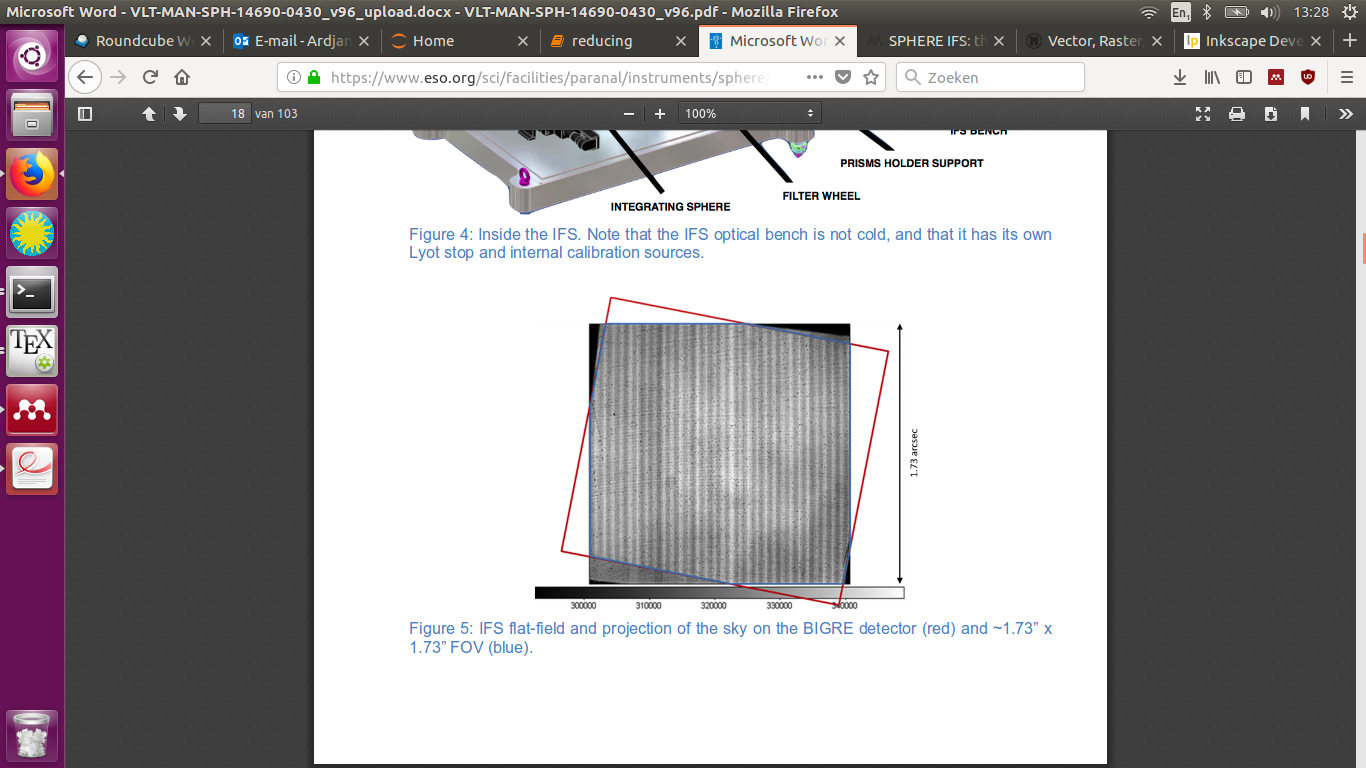
\includegraphics[trim={15cm 5.5cm 10cm 9.5cm},clip,scale = 0.47]{biggre}
\caption{IFS flat-field and projection of the sky. In the red the arrangement on the BIGRE detector and in blue the useful FOV. \citep{Observatory2007}} 
\label{fig:bigre}
\end{wrapfigure}

The IFS is able to obtain spectral information by use of BIGRE, an integral field unit consisting of 21000 microlenslets in a hexagonal grid, as displayed in Figure \ref{fig:bigregrid}. This grid is rotated by $10.7^o$ with respect to the dispersion in order to get the most lenslets stacked on the grid. This causes that a small section of the detector is meaningless, Figure \ref{fig:bigre}. The spectra of these lenslets are projected on the detector in a rectangular area with dimensions 5.1 x 41 pixels. 


\begin{figure}[htbp]
\centering 
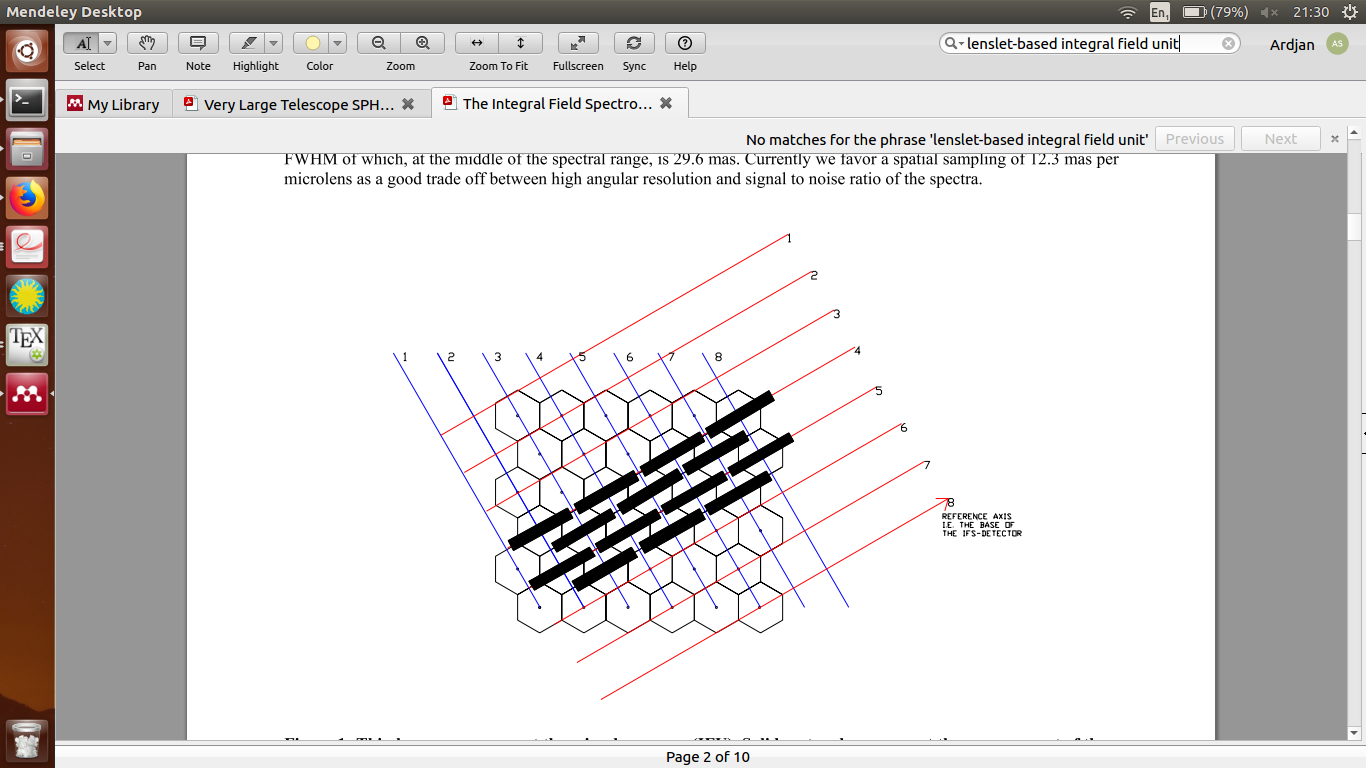
\includegraphics[trim={15cm 1.5cm 10cm 8cm},clip,scale = 0.47]{bigregrid}
\caption{The hexagonal lines represent the different microlenses of the IFU, the solid rectangles represent the spectra of the lenslets on the detector. The numbered lines  represent the orientation of the IFS Detector \cite{Claudi2008}} 
\label{fig:bigregrid}
\end{figure}

\subsection{Detector}
The detector of the IFS is 2048x2048 pixels. It is a standard infrared detector, since all light with a longer wavelength than the biggest wavelength in that mode is blocked. This light is blocked by use of a filter that has a sharp cut-off at the desired wavelength. It is technically possible to block longer wavelengths by us of the cut-off wavelength at which an HgCdTe detector is no longer sensitive, but this would make the instrument unnecassary complex and would increase the readout noise drastically from ~10 $e^-$ to ~25$e^-$\citep{Claudi2008}.
\bigskip

The detector is cooled with liquid Nitrogen, which reduces the thermal noise of the detector. The thermal noise of the cooled detector can be neglected with respect to dark noise in the instrument, photon noise of the observed star and other noise sources\citep{Claudi2008}. The detector is static and does not need to be rotateble since the rotation of the field and the pupil are corrected in the derotator. 

\subsection{Calibration devices}
The IFS has two calibration arms to provide a proper calibration of the instrument. The first arm is mounted in the common path and consists of a few calibration lamps. These lamps can be used to measure the througput of the lenslet grid and the different optical components in the IFS itself. Four additional lasers with wavelengths of respectively 0.9877, 1.1237, 1.3094 and 1.5451($\mu m$) are also provided on this calibration arm for the wavelength calibration. Each of the lasers is focused by the IFU on a different part in the spectra on the detector. Interpolation between these points gives an accurate model for the wavelength solution for each pixel, which can be used to reduce the data.
\bigskip

The second calibration arm is mounted internal to IFS, after the IFU, such that flats can be taken that measure the sensitivity of the whole detector. This is not possible with the external calibration lamps, since the detector has bigger dimensions than the FOV of the lenslet grid. decoupling the noise of the IFU and the detector makes the calibration slightly better and this allows to take calibration frames simultaneously to IRDIS, making the process of taking calibration data much faster. The internal calibration arm consist out of five calibration lamps: four narrowband lamps, centered around 1.0, 1.2, 1.3 and 1.5 $\mu m$, with a full width half maximum (FWHM) of about 0.01-0.04 $\mu m$ and one broadband white lamp\citep{Desidera}. An integrating sphere is also provided that spreads the light of the different lamps evenly over the whole detector.

\chapter{Methodology}
\section{IFS reduction for dummies}
Data taken with an integral field spectroscope contains for each pixel a spectrum, Figure \ref{fig:rawdata}. To reduce this to a cube with a frame for each wavelength bin, Figure \ref{fig:reduceddata}, several calibrations were needed. At first the dark current had to be subtracted and all pixels had to be corrected for their sensitivity using detector flat frames. After that the different spectra had to be located and the wavelength of all pixels calibrated. 

\begin{figure}[hb]
\centering
\begin{subfigure}{.5\textwidth}
  \centering
  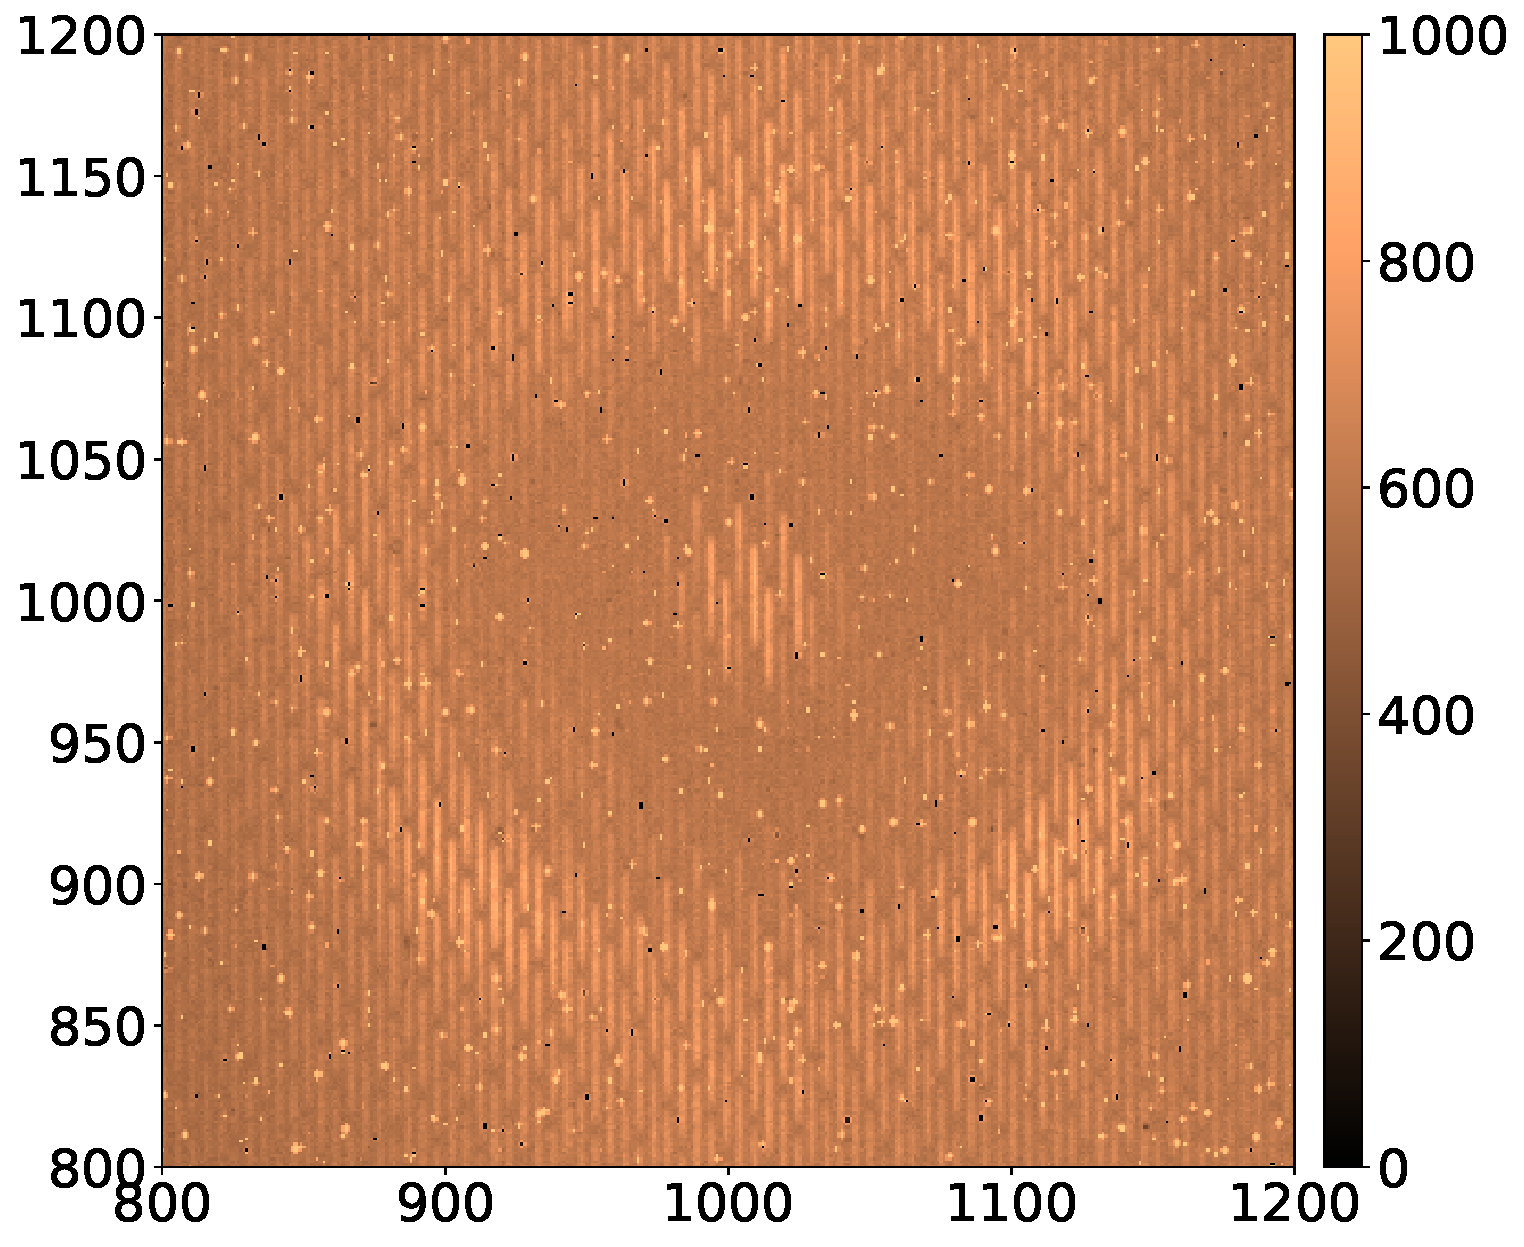
\includegraphics[width=1\linewidth]{rawframe}
  \caption{zoom of a raw science frame}
  \label{fig:rawdata}
\end{subfigure}%
\begin{subfigure}{.5\textwidth}
  \centering
  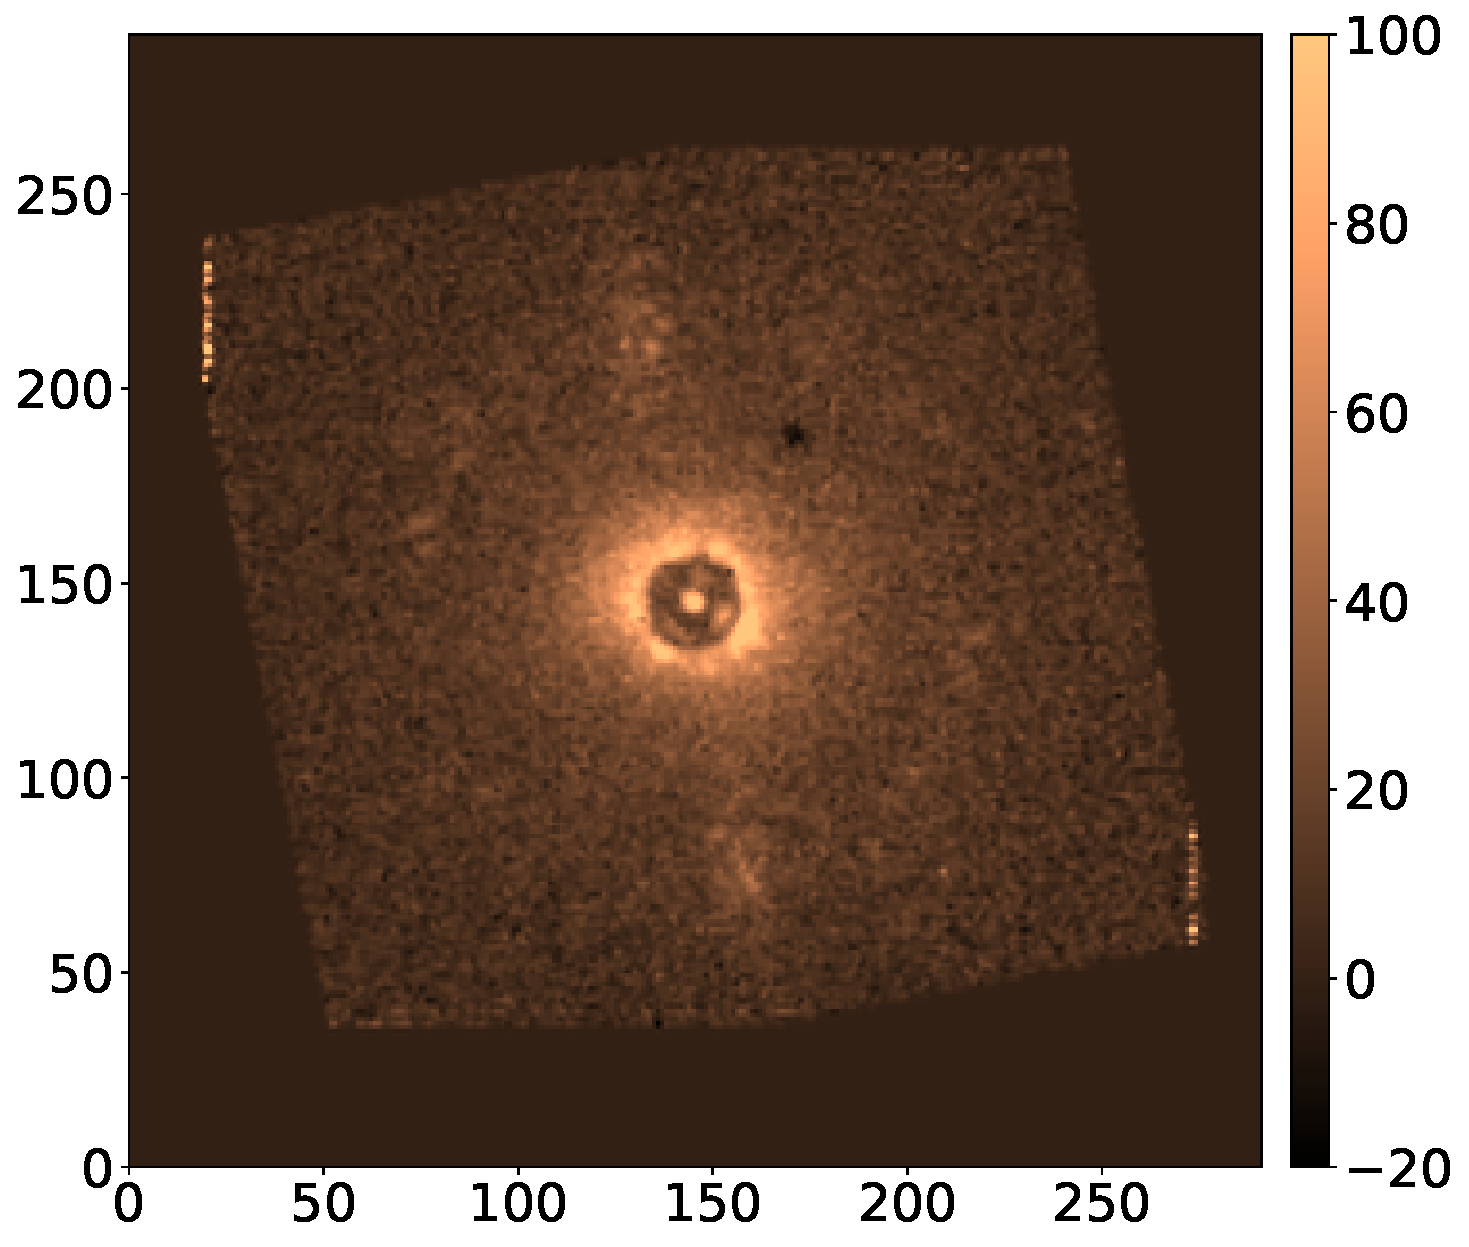
\includegraphics[width=1\linewidth]{reducedframe}
  \caption{one of the 39 reduced science frame}
  %\label{fig:sub2}
\end{subfigure}
\caption{the result of the basic reduction}
\label{fig:reduceddata}
\end{figure}

After correcting for the througput of the lenslet grid, the science reduction produced the final result with 39 spectral channels, each with a dimension of 291x291 pixels.
\bigskip

The Common Pipeline Library (CPL)\citep{Observatory2007} is a library of commands that is able to do the basic reduction steps of SPHERE data. Running the CPL can be done by use of Esorex, which is a commandline driven package, or EsoReflex that provides an easy and flexible way to run the different recipes of the pipeline. Esorex requires the use of a set of frames (sof) file for each recipe. This can easily be automized using Python, but since it is much work to write a code that identifies the different calibration images and mistakes can easily be made in the selection of the required data, I have used EsoReflex for the reduction and I really recommend using EsoReflex in the future. EsoReflex provides a user interface in the form of a workflow with a setup of a basic reduction pipeline in advance, which can be adapted in an easy way. It identifies all the required data that is unsorted stored in the input directory and gives a warning if something is missing. 
\bigskip

The data needed for a basic reduction is listed in table \ref{Tab:data}. Note that all the data has to be taken in the same mode, YJ or YH, as the science frames. All calibration data needs a corresponding dark frame with the same exposure time. The detectorflats however are taken with many different exposure time. In order to deal with this, two detector flats are needed per calibration lamp with different exposure times. The flat with shortest exposure time acts in the reduction as a dark and bias frame for the other one. This is possible since the flats give relative values by which the pixels have to be divide to measure uniform light, so the values are typical close to one. 
\bigskip

All individual reductions of calibration data have an own recipe in the common pipeline. A good understanding of these recipes and the corresponding calibration files is useful to get clean results in the end.

\begin{longtable}{| p{.20\textwidth} | p{.12\textwidth} | p{.58\textwidth }|}
\hline
\textbf{data type} & \textbf{number} & \textbf{comments}\\\hline
science frames&  &can be multiple frames stacked together as a single file with .fits extension.\\\hline
spectral positions & 1 & exposure time of 1.6507260s$^*$	\\\hline	
wavelength calibration & 1 & exposure time of 1.6507260s$^*$ \\\hline
detectorflat lamp 1 & 2 & two different exposure times\\\hline
detectorflat lamp 2 & 2 & two different exposure times\\\hline
detectorflat lamp 3 & 2 & two different exposure times\\\hline
detectorflat lamp 4$^{**}$ & 2 & two different exposure times\\\hline
detectorflat lamp 5 & 2 & two different exposure times\\\hline
instrument flat & 1 & \\\hline
background calibration & 1 & same exposure time as the science frames\\\hline
dark & & for all calibration frames one with corresponding exposure time\\\hline
\caption*{\\$^*$ shortest exposure time possible\\ $^{**}$ only if science data is taken in YH mode}\\% needs to go inside longtable environment
\caption{Data needed for the reduction of a science frame}%
\label{Tab:data}
\end{longtable}%

\subsection{Master dark}
The master dark recipe median combined multiple raw dark frames into one master dark. This recipe determines from the master dark the position of pixels that give strange results in all measurements, which are called static bad pixels. It returns both a file that contains a master dark frame, consisting of the image, bad pixels, the rms and the weightmap and a file that contains a static bad pixel map, which has the same content as the second extension in the master dark frame. An example of a master dark is showed in figure \ref{fig:masterdark}. 
\bigskip

If a background calibration file is given to the final science reduction, the background calibration file is used to correct for the dark current. The difference between these two is small. The only difference is that a normal dark is taken in N\_NS\_OPAQUE infrared IRDIS coronagraph combination mode and a background calibration in N\_NS\_CLEAR, meaning that combination of coronographs used to take the data has changed. Since darks are taken with the shutter closed, there should be no difference between these two and it is actually unclear why they even have both. \cite{Mouillet2013}

%I need some more text here above for my pictures. I need some more text here above for my pictures. I need some more text here above for my pictures. I need some more text here above for my pictures. I need some more text here above for my pictures. I need some more text here above for my pictures. I need some more text here above for my pictures. I need some more text here above for my pictures. I need some more text here above for my pictures. I need some more text here above for my pictures. I need some more text here above for my pictures. I need some more text here above for my pictures. I need some more text here above for my pictures. I need some more text here above for my pictures. I need some more text here above for my pictures. I need some more text here above for my pictures. I need some more text here above for my pictures. I need some more text here above for my pictures. I need some more text here above for my pictures.

\begin{figure}[!htbp]
\centering
\begin{subfigure}{.5\textwidth}
  \centering
  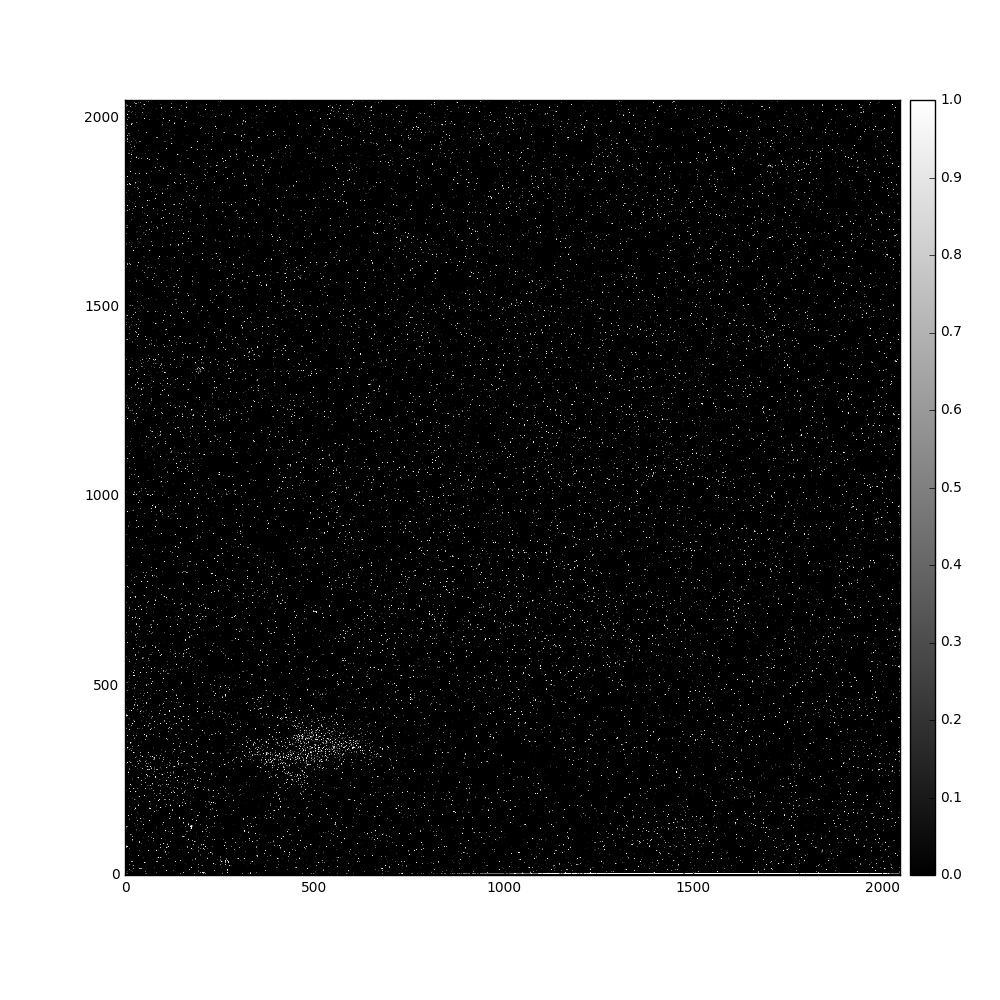
\includegraphics[width=1\linewidth]{badpixelmap}
  \caption{bad pixel map}
  %\label{fig:sub1}
\end{subfigure}%
\begin{subfigure}{.5\textwidth}
  \centering
  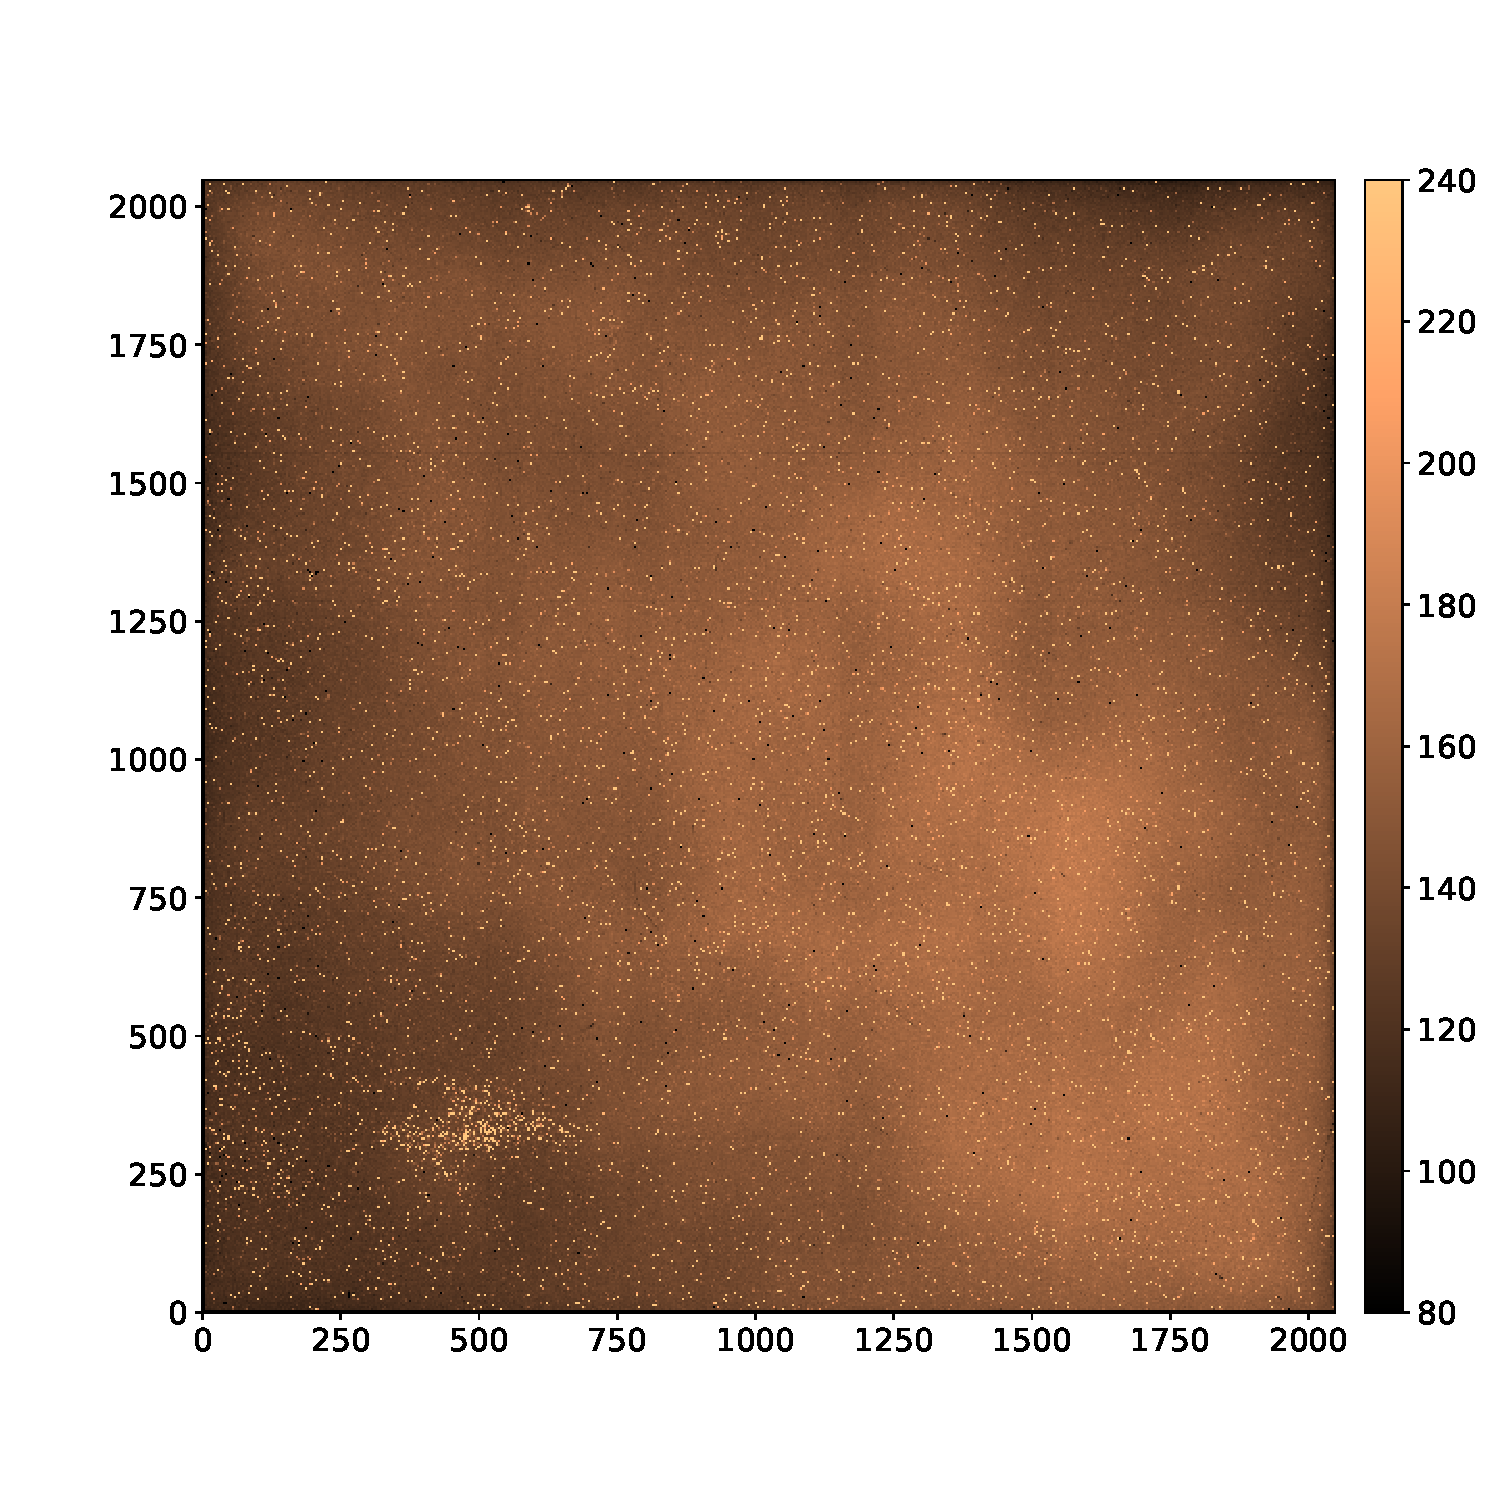
\includegraphics[width=1\linewidth]{dark}
  \caption{master dark}
  %\label{fig:sub2}
\end{subfigure}
\caption{result of the master dark recipe}
\label{fig:masterdark}
\end{figure}

\subsection{Detector flat}
\begin{figure}[!b]
\centering
\begin{subfigure}{.5\textwidth}
  \centering
  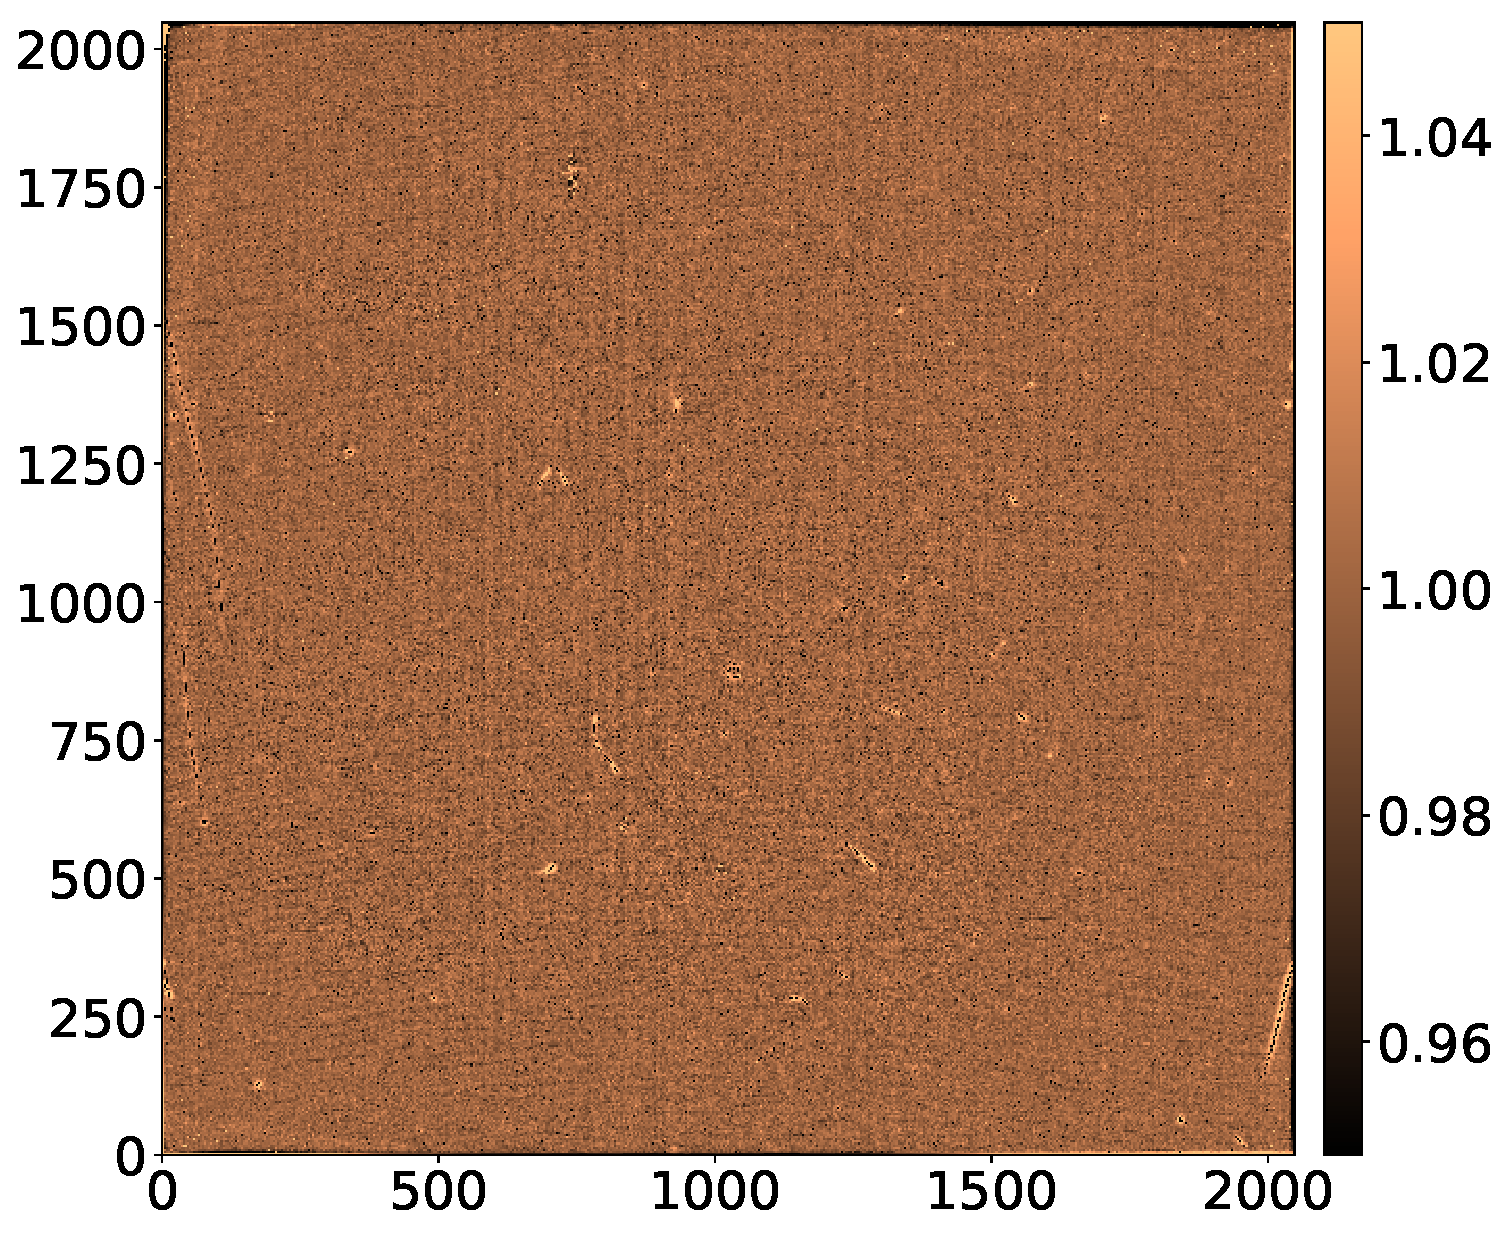
\includegraphics[width=1\linewidth]{masterdetectorflat}
  \caption{master detector flat}
  \label{fig:masterdetectorflat}
\end{subfigure}%
\begin{subfigure}{.5\textwidth}
  \centering
  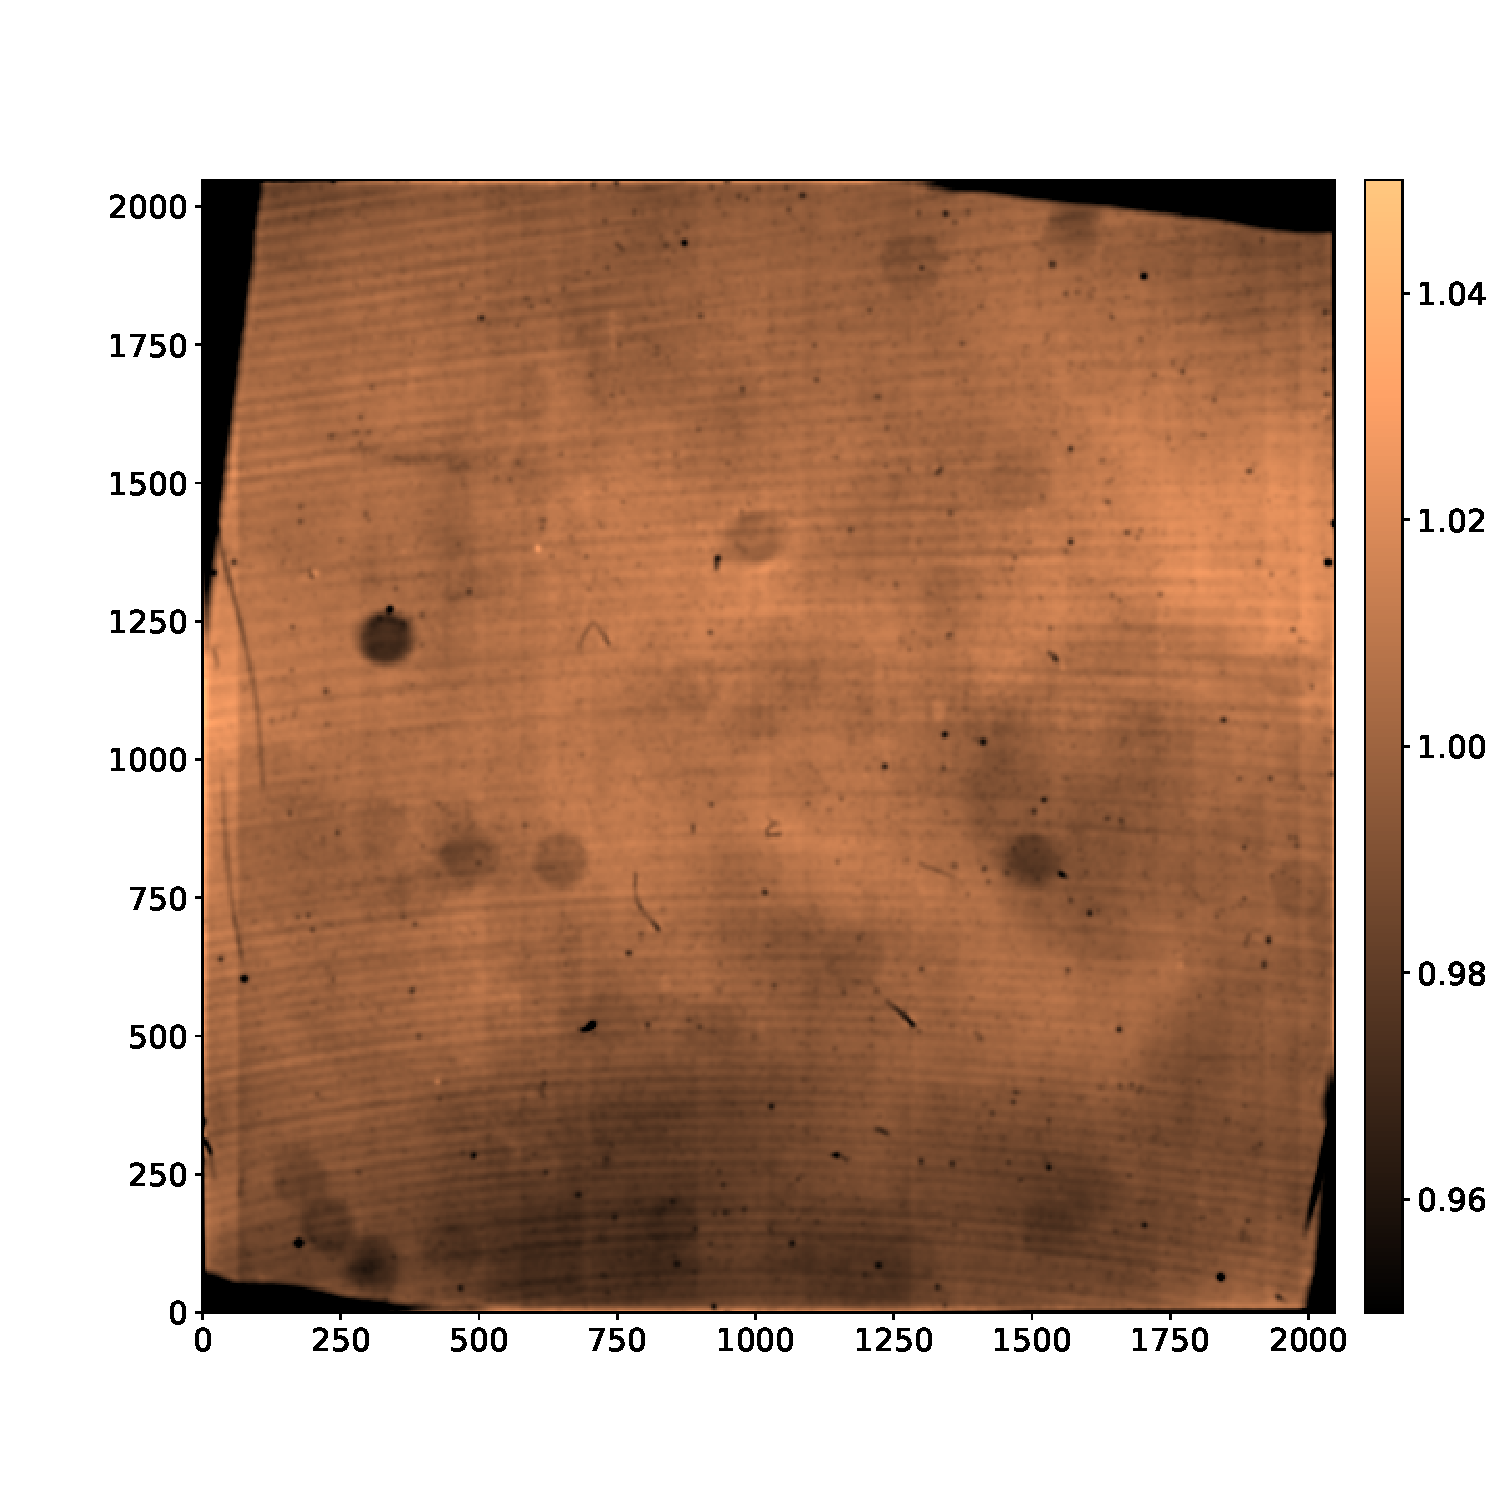
\includegraphics[width=1\linewidth]{largescaleflat}
  \caption{large scale flat}
  \label{fig:largescaleflat}
\end{subfigure}
\caption{result of the detector flat recipe}
%\label{fig:masterdark}
\end{figure}
At this step, the variation in sensitivity of the different pixels on the detector was measured. This can be done by using the extreme useful ability of the IFS to obtain flats with the shutter of the instrument closed and one of its internal calibration sources turned on. This means that the detector can be illuminated directly, which enabled us to correct better for the distortions of the detector itself. The distortions in the optical path are measured in the recipe that produces the instrument flat, described in the next paragraph. 
\bigskip

Since the IFS uses a range of wavelengths, different detector flats are needed, taken in different wavelengths to calibrate all pixels properly. The recipe returns the combined master flat frames for the different lamps that are used. The best flat to use in the rest of the recipes are the master detector flats Figure \ref{fig:masterdetectorflat}. Large scale flats are master flat frames that are smoothed with a gaussian. On this images the large scale dependences get visible, such as ghosts. Large scale flats can be used as a calibration file for the actual detector flat recipe, but since this effect is so small, it is left out in our reduction. One of the large scale flats is shown in figure \ref{fig:largescaleflat}

\subsection{Instrument flat}
\begin{figure}[!b]
\centering
\begin{subfigure}{.5\textwidth}
  \centering
  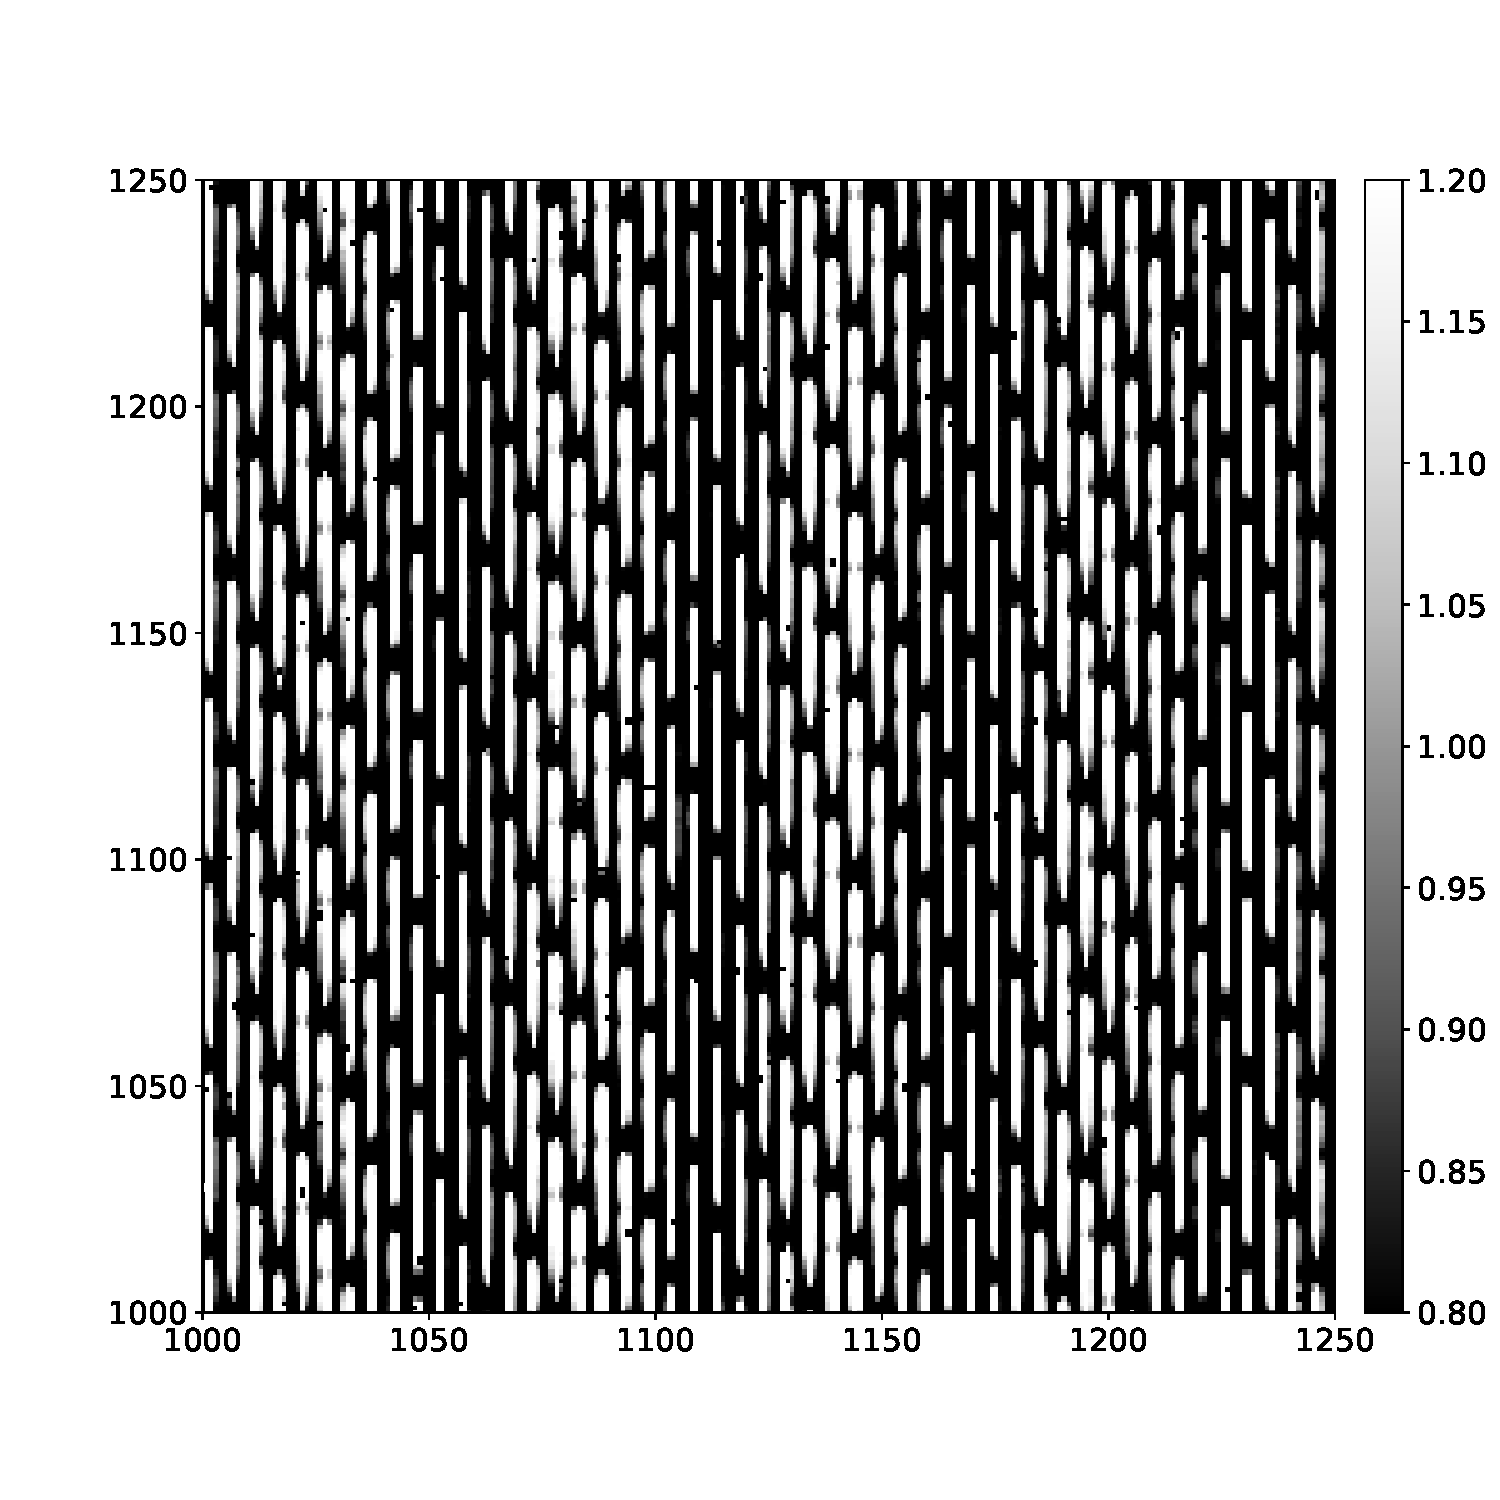
\includegraphics[width=1\linewidth]{instrumentflat}
  \caption{zoomed instrument flat}
  %\label{fig:preampflat}
\end{subfigure}%
\begin{subfigure}{.5\textwidth}
  \centering
  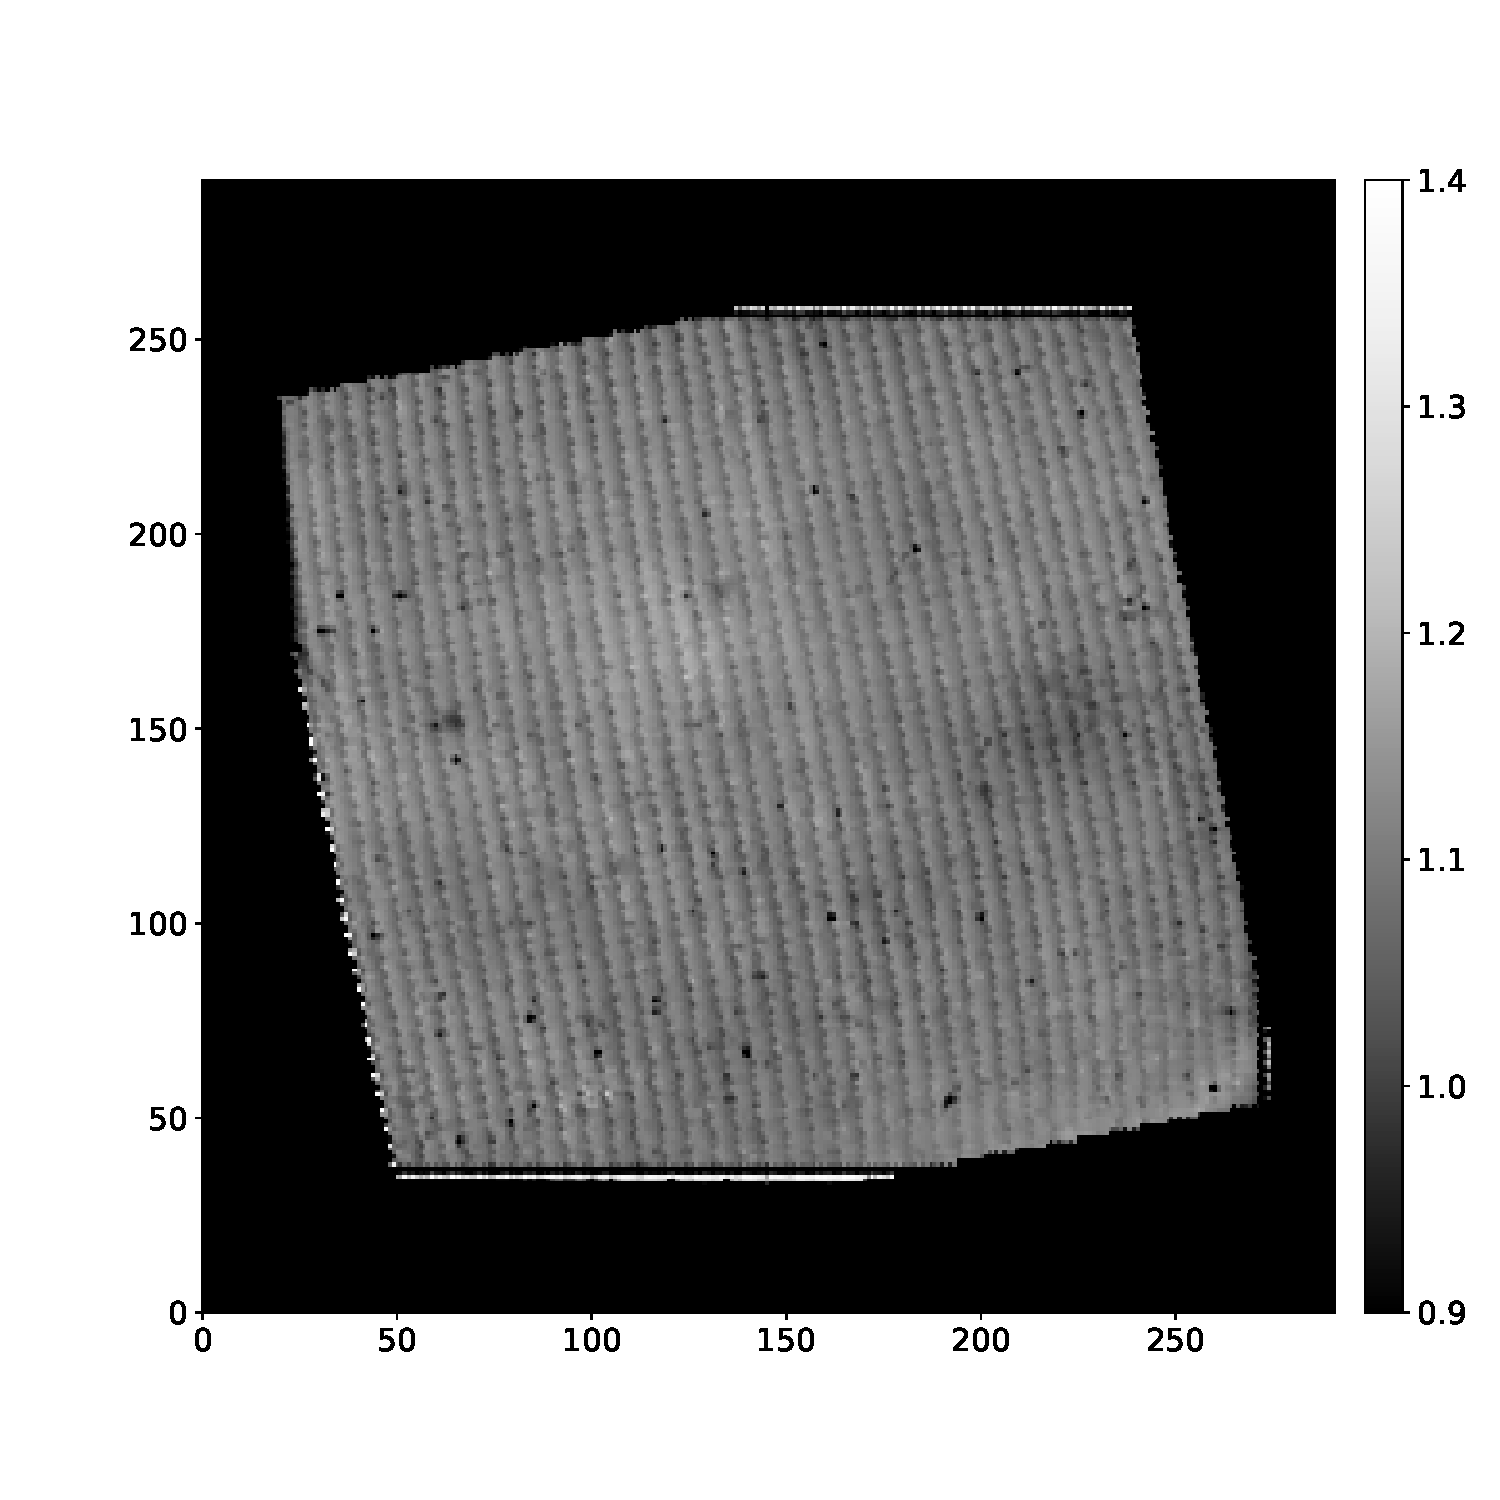
\includegraphics[width=1\linewidth]{IFU_flat}
  \caption{IFU flat}
  %\label{fig:largescaleflat}
\end{subfigure}
\caption{result of the instrument flat recipe}
\label{fig:instrumentflatrecipe}
\end{figure}
Instrument flats are obtained by taking a flat with three or four of the external calibration lamps on and is used to correct for the varying througput in the common path of the telescope and the instrument. After the dark subtraction, the flat field is divided by the detector flat, what has the effect of removing the detector response. This recipe returns both an instrument master flat which is the combined and reduced flat field before removing the detector response and the response of the integral field unit (IFU), which is the flat field after removing the detector response. The first can be used only for calibrating other calibration data, the latter can be used to reduce science data. The IFU flat field can be produced only if a reduced wavelength calibration is given. The production of the instrument flat is already possible with the positions of the spectrums only and is used to correct for the distortion of the lenslet grid in the wavelength calibration. The IFU flat does not give all pixels a sensitivity value, but assuming that most of the spatial distortion is due to the lenslet grid, the recipe returns the response of each individual lenslet. It gives for all pixels in the same spectrum a median value. This is why the IFU flat contains a typical stripe like feature. Both the IFU flat and the instrument flat are shown in figure \ref{fig:instrumentflatrecipe}. 

\subsection{Spectra positioning}
\begin{figure}[!b]
\centering
\begin{subfigure}{.5\textwidth}
  \centering
  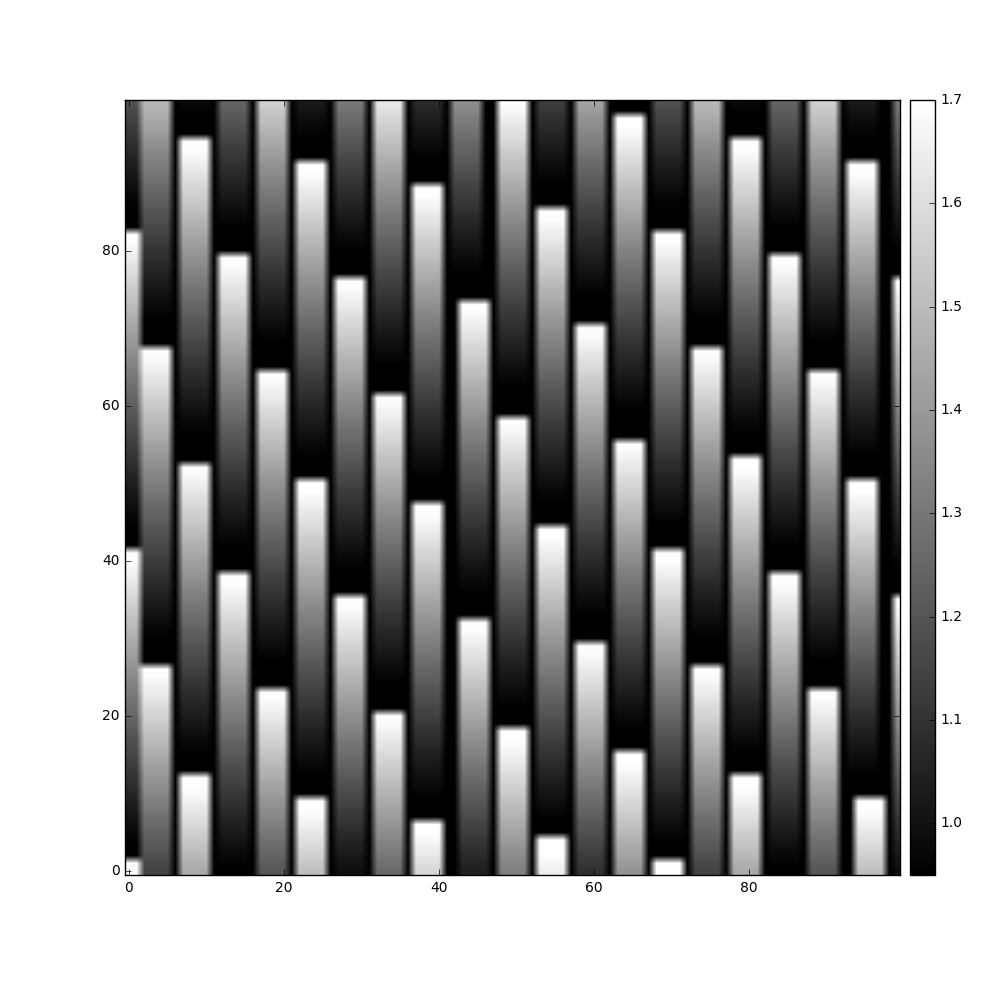
\includegraphics[width=1\linewidth]{specpos}
  \caption{zoomed positions of the spectra}
  \label{fig:specpos}
\end{subfigure}%
\begin{subfigure}{.5\textwidth}
  \centering
  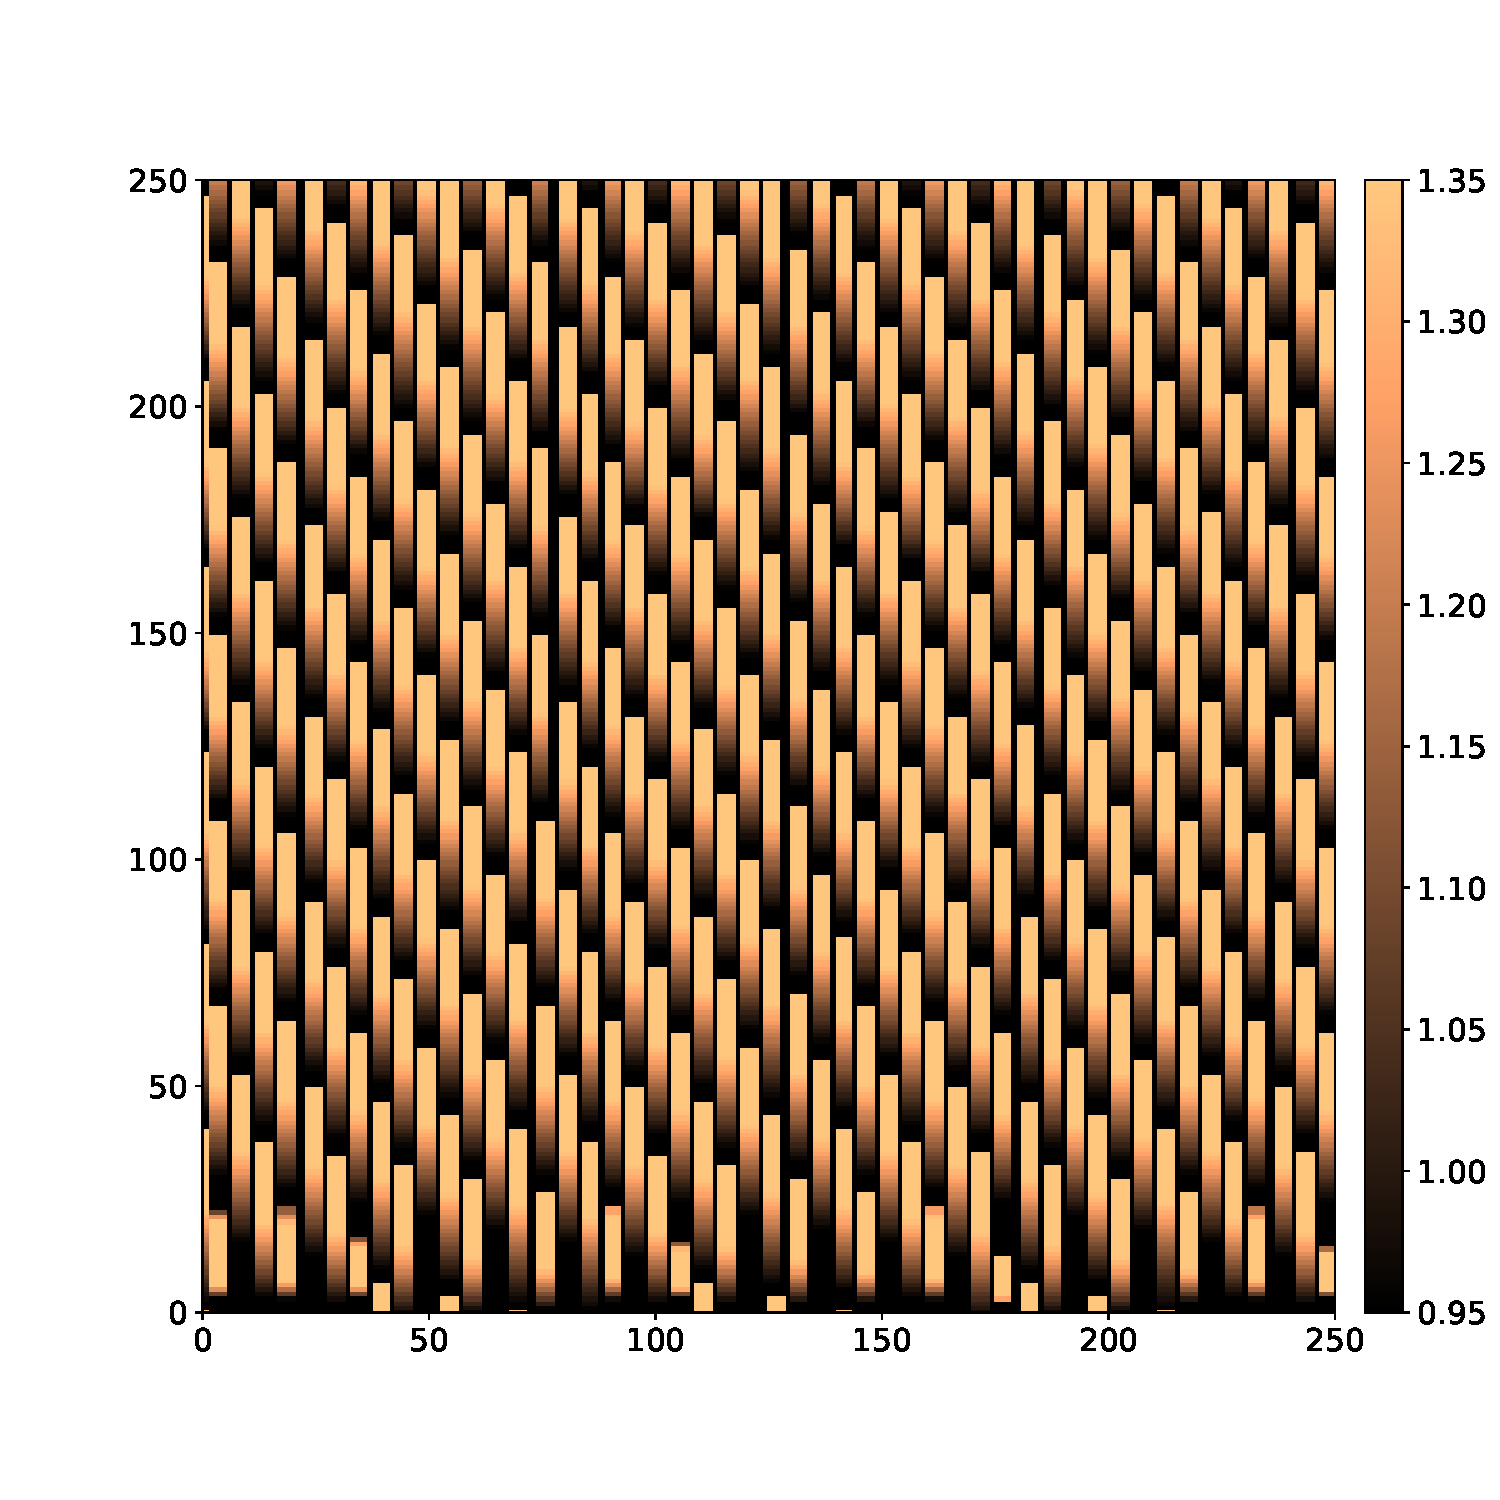
\includegraphics[width=1\linewidth]{wavecalib}
  \caption{zoomed wavelength calibration}
  \label{fig:wavecal}
\end{subfigure}
\caption{}
%\label{fig:masterdark}
\end{figure}

The spectra positioning recipe determines the exact position of the different spectra on the ccd with an accuracy of about 4 $\mu m$, i.e. 0.2 pixel\citep{Desidera}. This is enough to build a map with the location of the spectra, associating each pixel to an individual lenslet. It associates pixels with wavelengths according to a lenslet model. Note that this is a non-linear model, as is visible in \ref{fig:specpos}. Each pixel in this image has the value of the corresponding wavelength in micron. This model is just a good guess, the exact wavelength can be obtained by running the wavelength calibration. The seperation between the positioning of the spectra and the wavelength calibration makes the positioning of the spectra much better, which is the reason why they have split these steps in two different recipes. The raw calibration data for the spectra positioning recipe is obtained by illuminating the instrument with an external white calibration light source that is uniformly scattered by use of an integrating sphere that diffuses the incoming light, but preserves the power. A zoomed piece of the spectra positioning image is shown in figure \ref{fig:specpos}

\subsection{Wavelength calibration}
The wavelength calibration recipe refines the wavelength of the different pixels, by using data that is obtained by illuminating te instrument with three or four external lasers, emitting at 0.9877, 1.1237, 1.3094 and 1.5451($\mu m$). These lasers have been uniformly scattered with the same integrating sphere as mentioned in the section about the spectra positioning. The recipe tries to fit a spectrum on the positions that are determined in the spectra positioning recipe. Note that if a part of the spectrum does not fit on the ccd, the recipe is unable to fit a spectrum, which is visible in figure \ref{fig:wavecal}.

\subsection{Science reduction}
In the science reduction recipe the science frames are finally calibrated. This recipe needs all the output of the different calibration recipes as input alongside the raw science frames in order to correct properly for all the aberations. This recipe uses all the reduced calibration data in order to correct the data for all the different noise sources and asign pixels of the detector to pixels of the result in the end: a 39x291x291 datacube.

\section{Post-processing methods}
After the basic science reduction, the disk around the star is still unnoticable. Post processing techniques, based on subtracting a model of the stellar PSF were needed to gain the best result in detection of the disk. Two different methods are used to make a model for the stellar PSF: angular differential imaging (ADI) and spectral differential imaging (SDI). But before constructing a model for the PSF, the data needs to be centered correctly.

\subsection{Centering}
The telescope is calibrated such that the star is about in the center of the image, but there is always a slight offset. Center frames can be used to determine the center of the images on a level up to tenths of a pixel. These center frames are science frames containing also four artificial satellite spots, created by the adaptive optics system with the center of the star exactly in the middle of the four satellite spots, Figure \ref{fig:centerframe}. These center frames are usually taken before, during and after the science run, such that small changes of te center can be corrected. 
\begin{figure}[htb]
\centering
\begin{subfigure}{.5\textwidth}
  \centering
  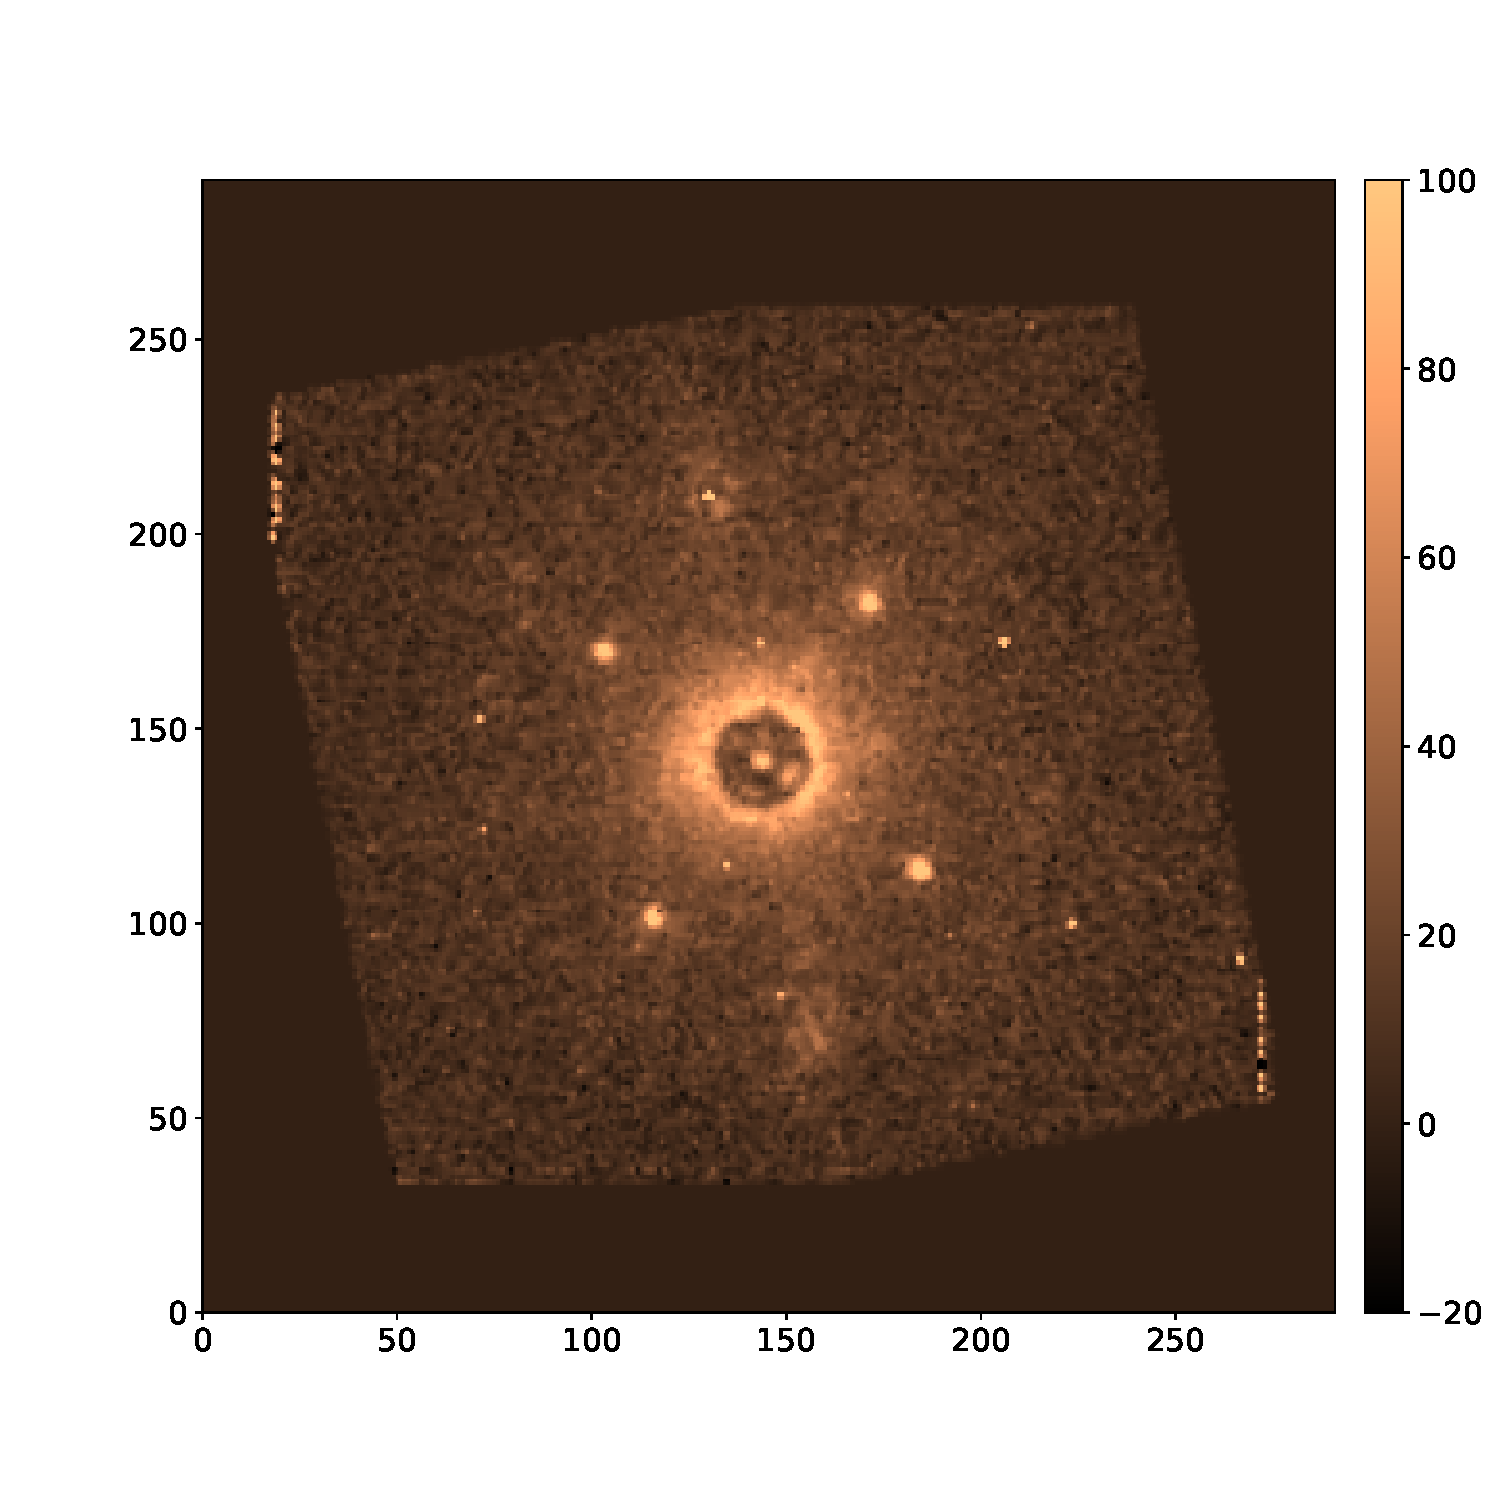
\includegraphics[width=1\linewidth]{centerframe}
  \caption{reduced center frame\\\\}
  \label{fig:centerframe}
\end{subfigure}%
\begin{subfigure}{.5\textwidth}
  \centering
  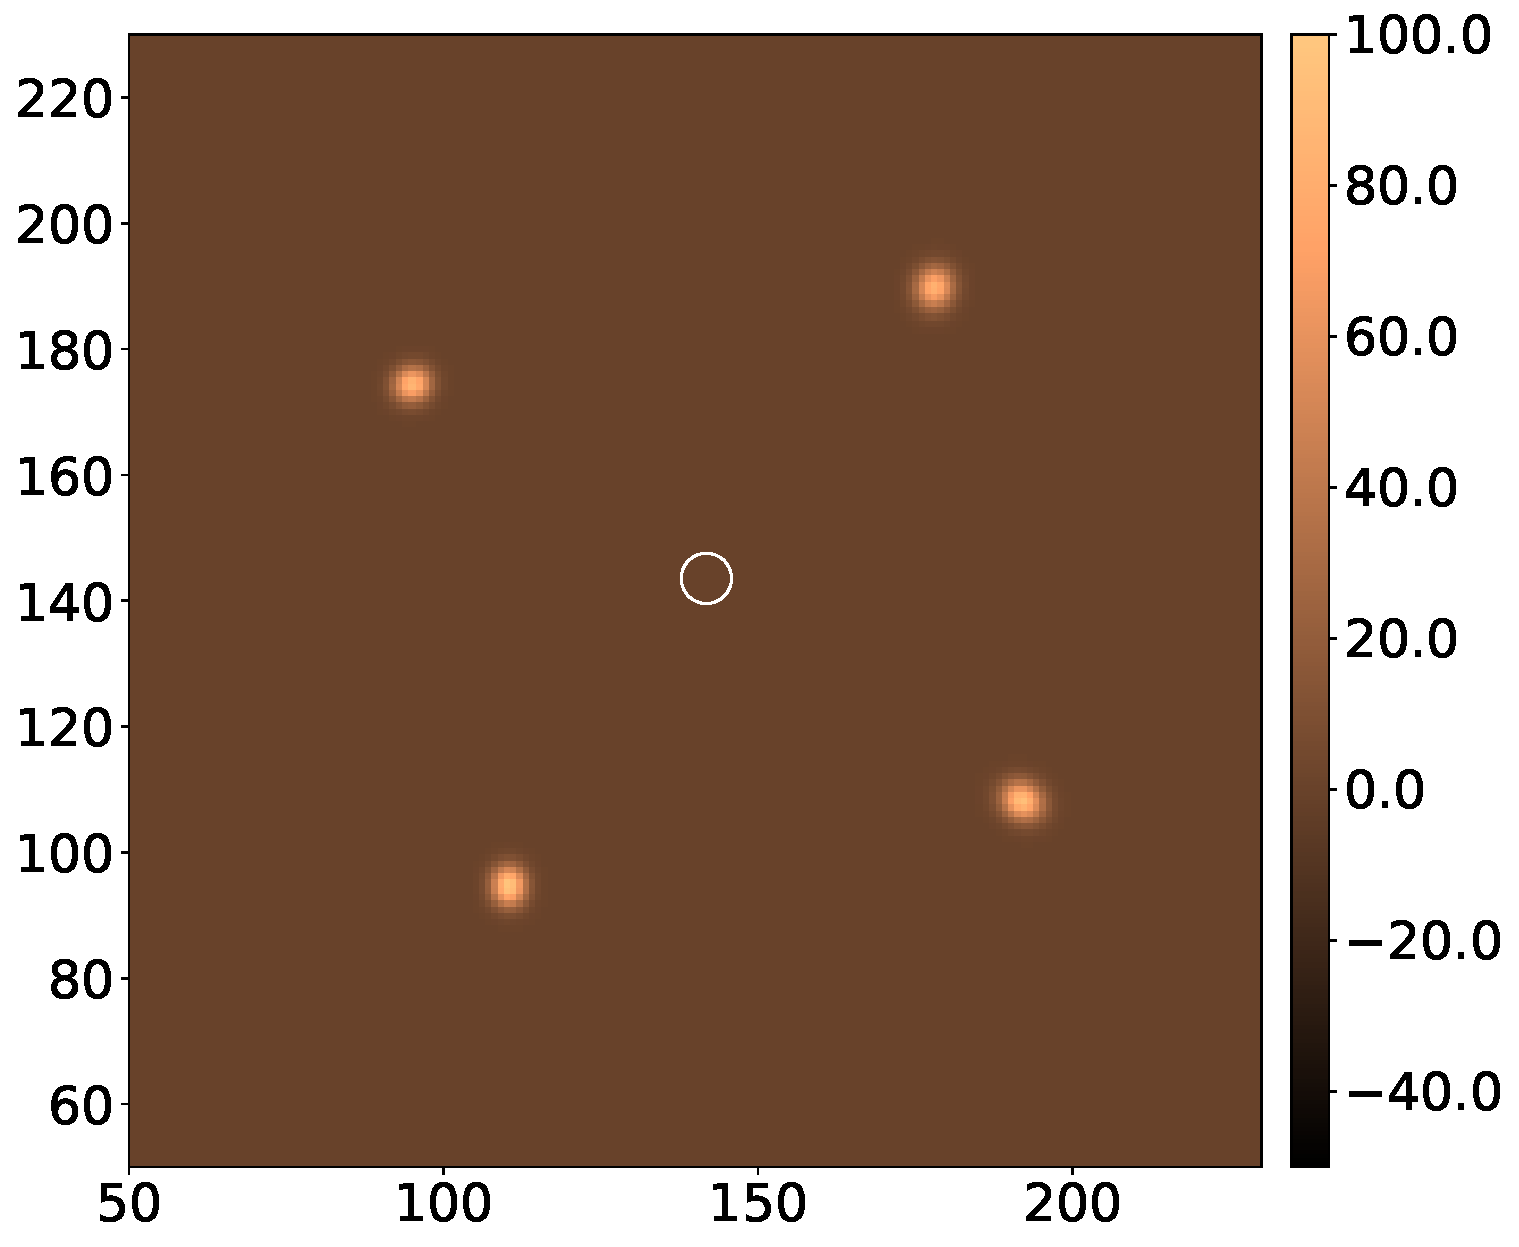
\includegraphics[width=1\linewidth]{centermodel}%
  \caption{model of the four satellite spots with the center of the star marked with a white circle}
  \label{fig:centermodel}
\end{subfigure}
\caption{}
%\label{fig:masterdark}
\end{figure}

\bigskip
Center frames are reduced in the same way as normal science frames, using the same dark and flat frames. Then the image is first smoothed with a gaussian with a standarddeviation of 25 that filters all the high frequency noise out and leaves a clean image of the four satellite spots. After that a single gaussian is fitted over each of the four satellite spots and a model is created for the combined satellite spots. The position of the center can be determined from the positions of the fitted gaussians. The fit of all the satellite spots on the centerframes were good, leaving almost no residue after subtracting the model from the data, as displayed in Figure \ref{fig:resultmodel}

\begin{figure}[!t]
\centering 
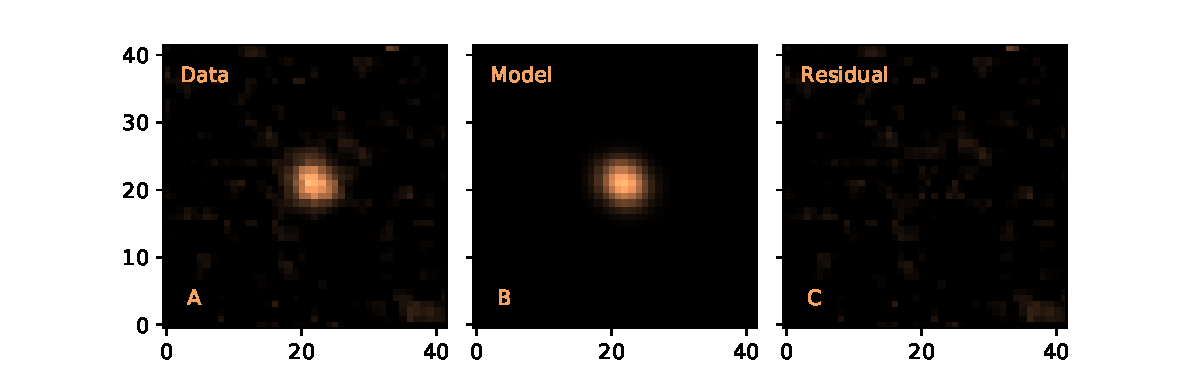
\includegraphics[width = \textwidth]{resultmodel}
\caption{\textbf{A:} one of the raw satellite spots, \textbf{B:} model of the satellite spot,\\ \textbf{C:} residual after subtracting the model of the data} 
\label{fig:resultmodel}
\end{figure}

\subsection{Angular differential imaging}
ADI is a post-processing method that constructs a model for the stellar PSF out of the rotation of the field during the night.\cite{Marois2005} Normally, telescopes correct for the rotation of the earth and hence the rotation of the object on the detector. To apply ADI on data, this correction is switched off, such that the field rotates over time during the night. The PSF of the star

\begin{wrapfigure}{R}{0.6\textwidth}
\centering
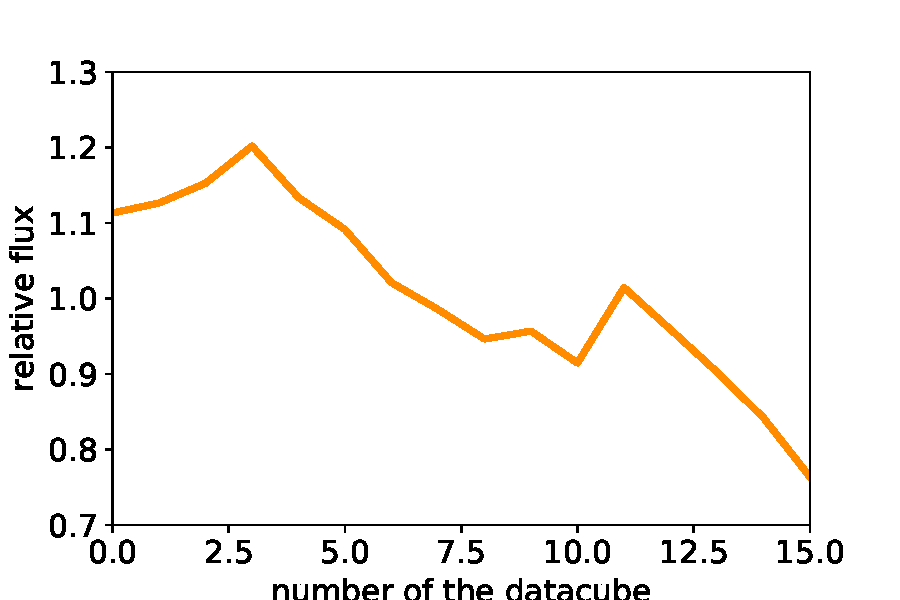
\includegraphics[width = 0.57\textwidth]{aonorm}
\caption{relative flux of the different datacubes over time}
\label{fig:aonorm}
\end{wrapfigure}

\noindent
does not change under rotation, since a star can be considered as a point-source, but the signal of the disk does. In the ultimate case is the disk signal therefore totally different in each frame. The total field rotation during the observation run was 69 degrees, in 16 different exposures, meaning that the signal has changed a lot on the detector over time. Taking the median per pixel, per wavelength over the whole time should hence give a model for the PSF of the star. Subtracting this model from each individual frame and relining the data with each other by rotating each frame with the known parallactic angle, gave good results. 
\bigskip

Since the data was taken with more than an hour between the first and last exposure, the flux of the object on the detector changes. This is partially due to changes in the sky during the night, but more due to changes in the quality of the correction of the adaptive optics during the night. To correct for this the median amount of flux in an annulus that grows in size with wavelength is measured, Figure \ref{fig:aonorm}. With this relative flux the PSF of the star in different exposures can be normalized such that it is correctly subtracted in each frame in the procedure. After the subtraction and before combination of de different frames, the normalization is reversed, such that the signal is not amplified in certain frames.


\subsection{Spectral differential imaging}

\begin{wrapfigure}{R}{0.6\textwidth}
\centering
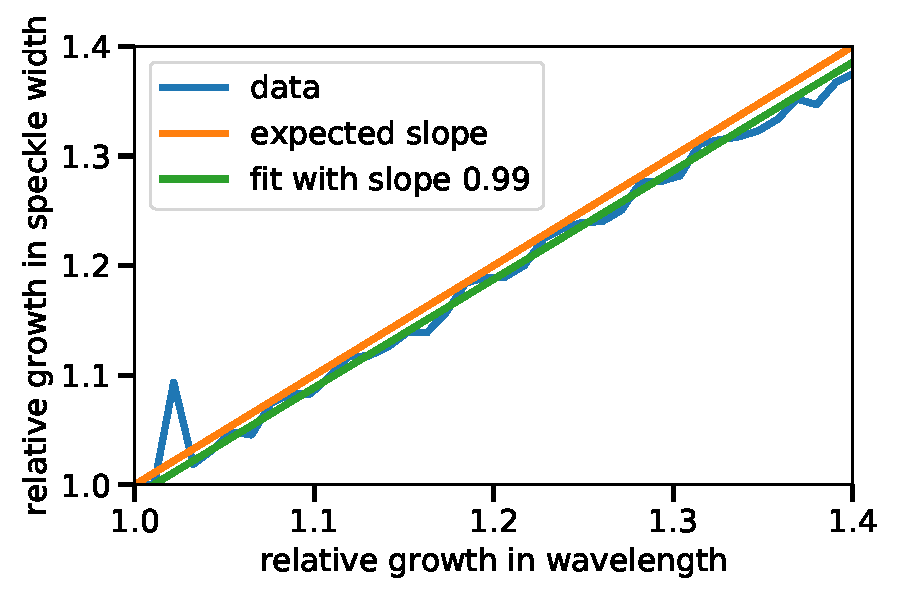
\includegraphics[width = 0.57\textwidth]{specklegrowth}
\caption{relative growth in the size of the PSF of the star versus wavelength}
\label{fig:specklegrowth}
\end{wrapfigure}
Spectral differential imaging is a post-processing method that constructs a model for the PSF of the star by use of the wavelength dependency of the PSF. Since the PSF of a star scales with $ \propto\lambda/D$, which means that the resolution and hence the scale of the PSF is directly proportional to the wavelength. We expect therefore that the PSF of the star increases linearly with wavelength. The signal of the disk however does not. In the ultimate case is the disk signal shifted to different pixels after rescaling such that the PSF of the star alligns in each wavelength. This should leave us with a model for the PSF after taking a median over all 39 spectral channels that does not contain anything of the disk signal. After subtracting this model from the data en scaling everything back to the original dimensions, such that the signal of the disk ligned up in each spectral channel, we got the best S/N ration. The different exposures have been combined by rotating them with the corresponding parallactic angle and then taking a median for each pixel in each spectral channel over the different exposures.
\bigskip

In order to check if the scale of the PSF is directly proportional to the wavelength, we measured the distance between the different artificially created satellite spots in the center image, using the same model as in the procedure that centers the science frames. The result of this measurement and the expected slope are plotted in Figure \ref{fig:specklegrowth}. This result indicates that the size of the PSF is indeed directly proportional to the wavelength, which means that the througput of the instrument does not spatially distort different wavelengths and that the wavelength calibration and positioning of the spectra is done in the right way.
\bigskip

\begin{wrapfigure}{R}{0.6\textwidth}
\centering
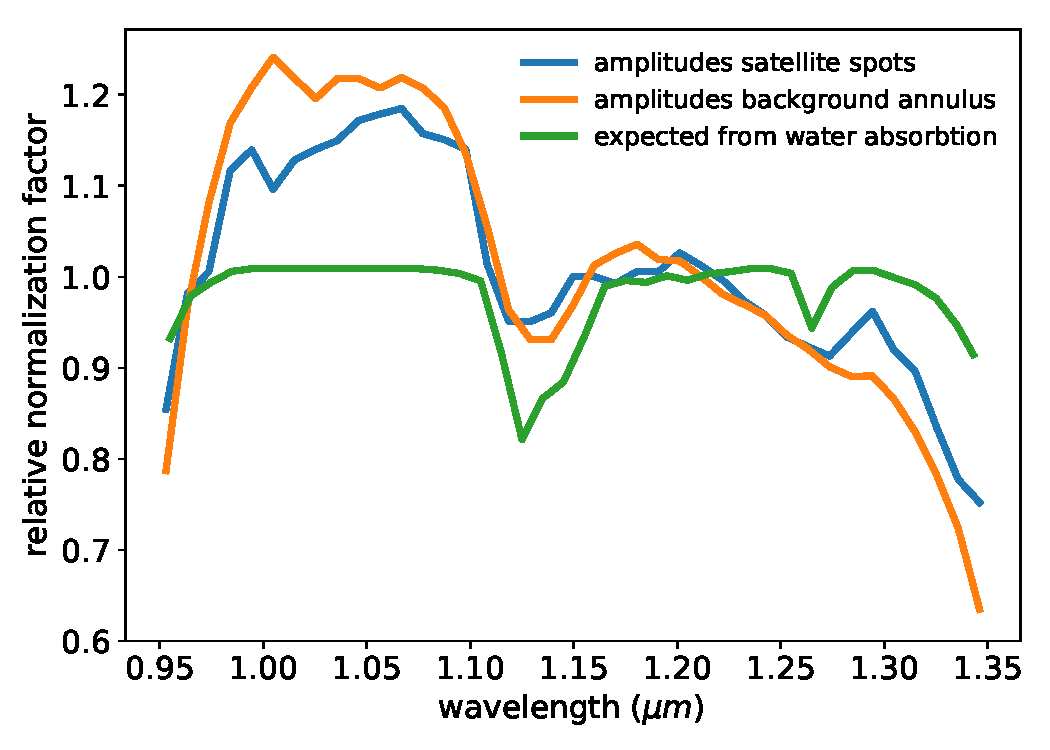
\includegraphics[width = 0.57\textwidth]{allnormalization}
\caption{relative growth in the size of the PSF of the star versus wavelength}
\label{fig:throughputnorm}
\end{wrapfigure}

\noindent
Just as in the angular differential imaging, the data needs to be normalized before we take the median in order to get a good model of the PSF in each spectral channel. Since the throughput of the atmosphere, the instrument and the common path of the telescope is wavelength dependent, we had to normalize the flux in the different spectral channels. Our first try was to average the amplitude of the four fitted gaussians over the satellite spots in the center frames, but this did not turn out that well. Secondly we tried to measure the flux in a fixed annulus around the center, after scaling the different spectral channels such that the PSFs lined up, Figure \ref{fig:throughputnorm}.
\bigskip

The normalization factor as derived in the second way mentioned differed just a little from the one using the center frames, but this left us with good results in the end. The dips in the normalization factors line up with the expected dips in the throughput of the atmosphere due to absorbtion, Figure \ref{fig:throughputnorm}, since there is a big abundance of strong absorbtion lines of water in that part of the spectrum. The general trend is a decreasing flux over wavelength. The star peaks in the H band \citep{Padgett}. This would indicate that the flux of the star should slighty increase over the range of the IFS. The decrease in flux is definitely due to wavelength dependencies in the throughput of the instrument as displayed in Figure \ref{fig:systemthrougput}. 

\chapter{Results}
\section{ADI}
\section{SDI}
\section{Spectral analysis}
\subsection{Signal over wavelength}
\subsection{Signal over azimuthal angle}

\chapter{Discussion}
\section{Comparing classical ADI with TLOCI}
\section{Comparing SDI and ADI results}
A big disadvantage of this method, is that it has often to deal with self-subtraction, meaning that the signal of the disk is subtracted by another part of the signal of the disk, leaving us with no detected signal. 
\section{Evaluation of SPHERE/IFS}





%\chapter{Spatially entangled 4-photons states from a periodically poled KTP crystal}

\framebox[\textwidth]{
\begin{minipage}[b]{.75\textwidth}
\vskip 0.5em
The contents of this chapter serve as an example and are based on a scientific paper published as Phys. Rev. A {\bf 85}, 043837 (2012). This article contains results from the master thesis of Alexander J.H. van der Torren. The results and data analysis of the original master theses have been reproduced, extended and improved by S. Cigdem Yorulmaz at a later stage.
\vskip 0.5em
\end{minipage}
}

\vskip 2em

Photon pairs produced via spontaneous parametric down-conversion (SPDC) in a non-linear crystal give rise to strong nonclassical correlations. The resulting entangled photons are an important resource in quantum information, fundamental tests of quantum mechanics and have been used in experiments that demonstrate the violation of Bell's inequality, quantum teleportation and quantum communication. While most experiments focus on discrete polarization entanglement, quantum states of two particles that are entangled in continuous variables~\cite{Braunstein:RMP2005} such as frequency~\cite{Ou1988,Li2009}, time-bin~\cite{Friberg1985,Ou1999,Riedmatten2004} or photon momenta~\cite{Strekalov1995,Law2004,Howell2004,Walborn2010} are also possible, which gives access to high-dimensional entanglement that can be explored by measuring correlations between two photons.

In this article, we focus on spatial entanglement using photon momenta as a continuous variable. Unlike other forms of continuous variable entanglement, the quantum correlations in spatial entanglement can be resolved with relative ease and high resolution by using a combination of lenses and apertures only. The low conversion efficiency in non-linear crystals combined with the long coherence time of a continuous wave pump and ultrashort coherence time of the photon pairs ensure that most experiments are well described by two-photon interference of individual pairs~\cite{Walborn2010}. As a consequence, spatial entanglement with more than two photons has remained elusive and spatial correlations beyond independent photon pairs have not been addressed in an experiment~\cite{Assis2011}. These multi-photon states are of interest since they provide access to non-trivial entanglement between more than two particles~\cite{Greenberger1989,Dur2000}. Furthermore, the generation rate of four photon states sets fundamental limits on the visibility achievable in two-photon interference experiments~\cite{Marcikic2002} and the maximum attainable key generation rate in quantum key distribution protocols.

Here we investigate events where four spatially entangled photons are generated by SPDC. These four photons can either be two independent pairs, or they may all be in the same set of spatial and temporal modes to create a true four-photon state~\cite{Ou1999,Riedmatten2004}. The production of these four photon states is enhanced by the physical process of stimulated emission of a second photon pair into the same optical mode as the first pair. In the ideal situation of a single temporal and spatial mode, stimulated emission enhances the pair production rate by a factor of two compared to the probability to generate four photons in the same mode via two independent spontaneous processes. For a multi-mode situation, the relative importance of the stimulated emission process is given by a ``visibility'' $\chi$ that ranges from 0 to 1.

The distinction between two independent pairs and four-photon states has been addressed in the time-domain using time-bin entanglement with a pulsed laser source~\cite{Ou1999,Riedmatten2004}. These experiments are restricted to a single spatial mode and therefore do not allow use of spatial degrees of freedom to explore the process of stimulated emission. The total number of modes is then given by the available temporal modes and is directly related to the frequency bandwidth of the SPDC light as compared to the frequency bandwidth of the pulsed laser source~\cite{Riedmatten2004}. To directly resolve the underlying mode structure requires a measurement of quantum correlations within a single laser pulse. Such a direct measurement of the arrival time would require detectors with high quantum efficiency and sub-picosecond timing resolution, which is well outside reach of current single-photon detector technology~\cite{Hadfield2009,Eisaman2011}. Instead, we use spatially entangled multi-photon states that allow us to resolve the fine structure of stimulated pairs emitted in a single laser pulse in a straightforward way. Using pinholes the momentum resolution in the far-field of the SPDC source may be made arbitrarily high. In an experiment, there is always a trade-off between the size of the pinhole and the collected signal, which sets the time required to measure coincidence rates to a sufficient level of accuracy.

\section{Stimulated emission of spatially entangled 4-photon states}

The downconversion process in the PPKTP crystal that generates photon pairs in $N$ spatial modes can be described by an interaction Hamiltonian of the SPDC process given by~\cite{Simon2000,Kok2000}:
\begin{equation}
H = \kappa \sum_{i}^N a^\dagger_{\vec{q_i}} a^\dagger_{\vec{-q_i}} + \mathrm{h.c.},
\end{equation}
where $a^\dagger_{\vec{q_i}}$ is the creation operator that creates a single photon in a spatial mode labeled by the transverse wavevector $\vec{q_i}$. The operator $a^\dagger_{\vec{q_i}} a^\dagger_{\vec{-q_i}}$ thus creates a pair of photons that is correlated in their transverse photon momenta and forms the basis for spatial entanglement. The parameter $\kappa$ describes the strength of the non-linear interactions and contains, among others, the (time-dependent) field of the pump and the effective non-linearity of the PPKTP crystal. For our purpose, where we pump the crystal with an intense pulsed laser, $\kappa$ can be assumed to be a classical  quantity. The corresponding wavefunction of the state generated by SPDC can be directly obtained from the Hamiltonian:
$$
\ket{\Psi} = \exp(-i H \frac{t}{\hbar}) \ket{0} \approx (1-\frac{i t}{\hbar} H - \frac{t^2}{2 \hbar^2} H^2) \ket{0},
$$
where we limited the Taylor expansion in the last step to exclude quantum states with more than 4 photons. The linear term in the Taylor expansion creates a state $\ket{\Psi_2}$ that consists of a superposition of a single photon pair in any of the available spatial modes:
$$
\ket{\Psi_2} = \frac{- i t}{\hbar}H \ket{0} = \frac{- i \kappa t}{\hbar} \sum_{i=1}^N \ket{1_{\vec{q_i}};1_{\vec{-q_i}}}.
$$
Please note that we use a shorthand notation in which we leave out all spatial modes without a photon. The spatial modes that contain photons are numbered by the number of photons in that mode and the subscript refers to the transverse photon momentum of that mode. The quadratic term gives rise to a state $\ket{\Psi_4}$ with 4 photons that contains all double pair contributions, which can be represented using the same notation~\cite{Riedmatten2004} as
\begin{eqnarray*} \ket{\Psi_4} & = & \frac{- \kappa^2 t^2}{2 \hbar^2} \bigg( 2 \sum_{i=1}^N \ket{2_{\vec{q_i}};2_{\vec{-q_i}}} + \\ & & \sum_{i=1}^N \sum_{j=1, i \neq j}^{N} \ket{1_{\vec{q_i}},1_{\vec{q_j}};1_{\vec{-q_i}},1_{\vec{-q_j}}} \bigg).
\end{eqnarray*}
The effect of stimulated emission follows directly from the creation operators and is contained in the extra factor $\sqrt{2}$ when two photon pairs are created in the same spatial mode.

A measurement of a single photon in a particular spatial mode with wavevector $\vec{q_i}$ determines the wavevector of the twin photon and corresponds to a state projection: $a_{\vec{q_i}}\ket{\Psi}$. The state projection allows us to calculate the probabilities of creating a single photon pair $P_2$ as well as the probability $P_4$ to create a state with 4 photons in the same mode. For a single spatial and temporal mode, the probability $P_4$ is exactly equal to $P_2^2$ and is thus enhanced by a factor 2 compared to stimulated emission of two photon pairs in the same spatial modes. In a situation with more than one spatial mode, which is of interest here, stimulated emission enhances the probability $P_4$ by a factor $(1+\chi)$, where $\chi$ is a ``visibility'' from 0 to 1 that quantifies the extra contribution to the 4 photon states due to stimulated emission. The probability to create a 4 photon state with the photons in the same mode can then be expressed as~\cite{Riedmatten2004}:
\begin{equation}
P_4 = \frac{P_2^2}{2} (1+\chi).
\end{equation}

\section{Experimental investigation of 4-photon quantum correlations}

\subsection{Experiment}

\begin{figure}[tbp]
\centering 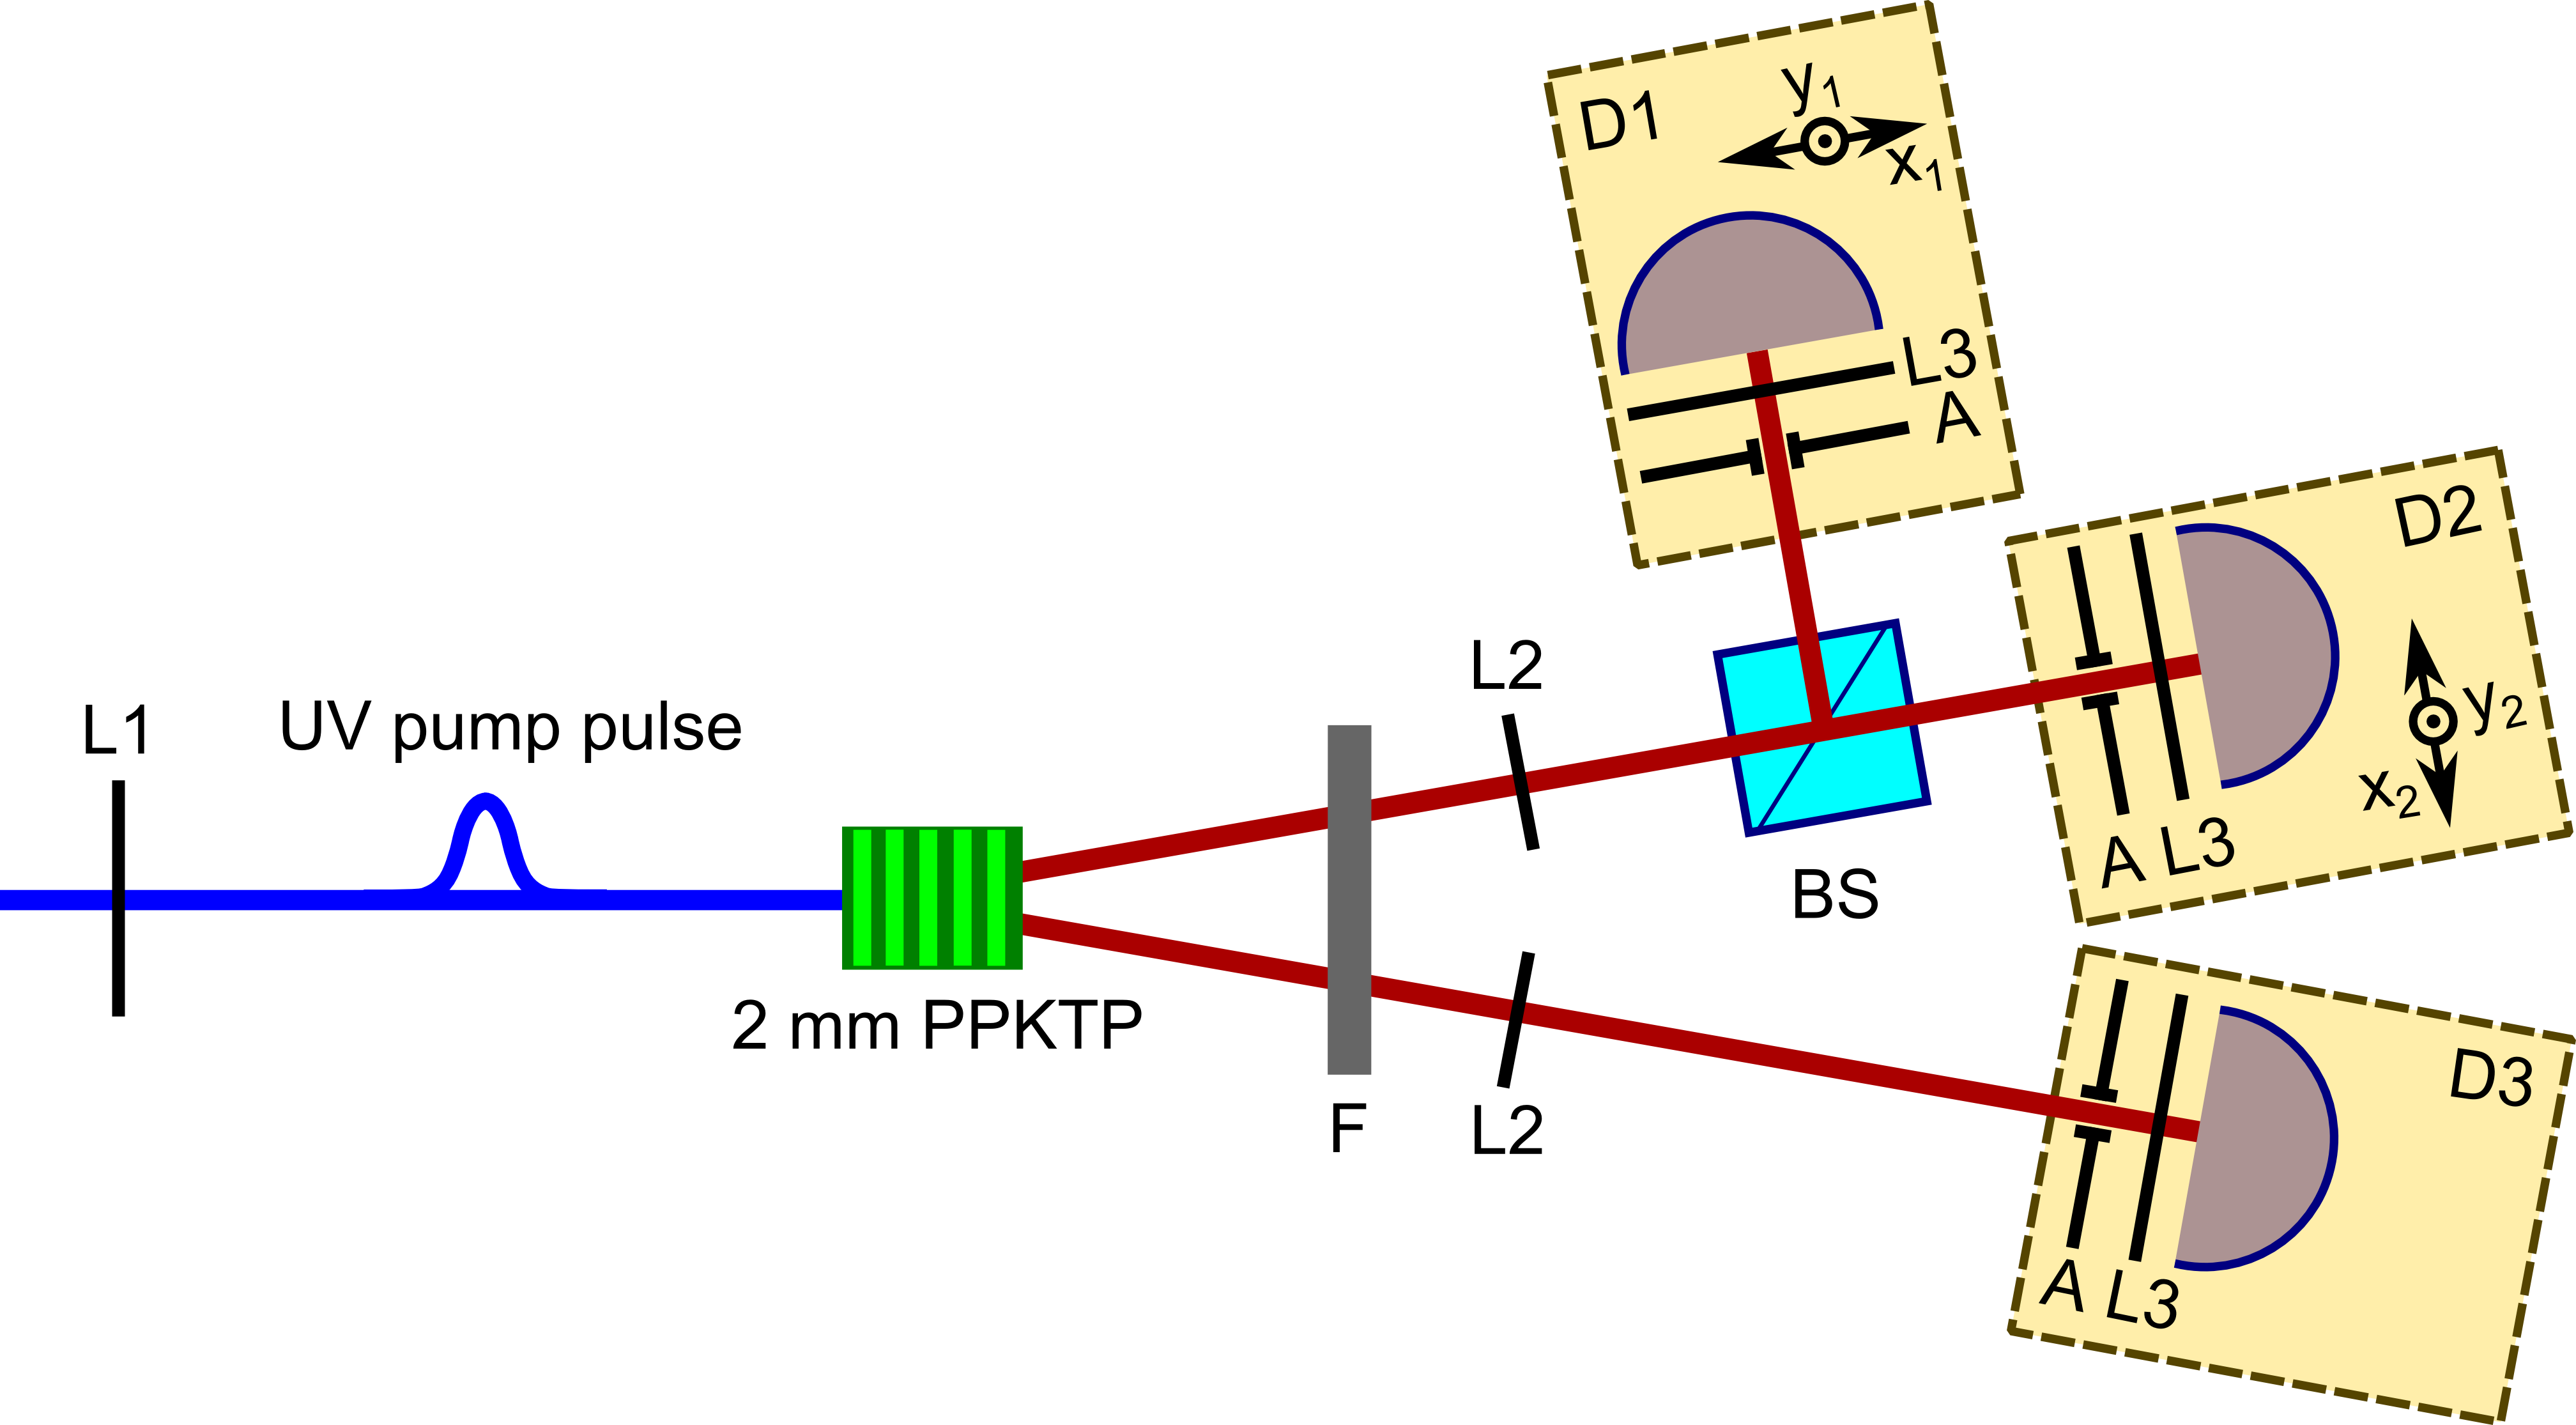
\includegraphics[width=120mm]{Fig1.png}
\caption{(Color online) Setup to measure spatially entangled 4-photon states via parametric downconversion in a 2 mm PPKTP crystal. UV pump pulses from a frequency doubled Ti:Sapphire laser are focused by lens L1 ($f_1$~=~250~mm). Photons are collected by the lenses $L2$ ($f_2$~=~270~mm) and detected by the detector assemblies $D1-D3$ that use photon counting APDs to detect single photons in a particular direction defined by the apertures $A$ placed in the combined focal planes of $L2$ and $L3$ ($f_3$~=~4.5~mm). The beamsplitter, $BS$, allows to record if two photons are in the same spatial mode. To this end detector assemblies $D1$ and $D2$ are placed on computer controlled translation stages. Correlations in the coincidence events are due to 4-photon states that are created by the process of stimulated emission of photon pairs.} \label{Fig:setup}
\end{figure}

Figure~\ref{Fig:setup} depicts the setup to explore the spatial quantum correlations due to stimulated emission of pairs in a four-photon state. In order to get a non-negligible rate of double pairs we use a highly efficient, 2 mm long, periodically poled KTP (PPKTP) crystal~\cite{Peeters2008} pumped by $\sim$100 mW of 413.2 nm pulsed laser light. The pulsed laser in our setup produces 2 ps pulses and is focussed into the PPKTP crystal using a lens $L1$, with a focal length $f$ of 250~mm. The source creates non-colinear, frequency degenerate photon pairs at a wavelength of 826.4 nm that are filtered by a bandpass filter $F$ and collected by lenses $L2$ ($f$~=~270~mm). Three detector assemblies $D1-D3$ are used to collect single photons with a well-defined momentum. Each of these assemblies consists of a lens $L3$ ($f_3$~=~4.5~mm), an aperture $A$ placed in the far-field to select the photon momentum and a (multi-mode) fiber-coupled single photon counting avalanche photodiode (Perkin-Elmer SPCM-AQ4C). The mode diameter of the fiber used in the experiments is $50$~$\mu$m and lenses $L2$ and $L3$ provide a 60$\times$ magnification factor. Coincidence detection with a $\sim$1.7~ns coincidence window between the detectors $D1$ and $D3$ (or $D2$ and $D3$) results in a measurement of spatial entanglement of single pairs. The beamsplitter, $BS$, allows us to record coincidence events between detectors $D1$ and $D2$ that are due to two photons from different pairs. To record the spatial correlations both detector assemblies $D1$ and $D2$ are placed on computer controlled translation stages that allow movement in the $x$ and $y$ directions transverse to the optical beam.

The essential feature of the setup is that it allows us to distinguish a genuine 4-photon state from two independent pairs by detecting coincidences between two photons in the same arm, as was introduced earlier for 4-photon states in the time-domain~\cite{Riedmatten2004}. In this setup only the 4-photon states created by stimulated emission generate strong correlations between detectors $D1$ and $D2$, while double pair states do not create any special correlations.

The length of the 2~ps laser pulse is a compromise between a short laser pulse to select a single temporal mode on the one hand and a somewhat longer laser pulse to retain efficient SPDC on the other hand. For a very short laser pulse the photons are created at a well-defined time, but the SPDC process becomes inefficient due to the broad spectral content of the laser pulse. In our study, the combination of the pulse duration and the bandpass filter selects $\sim$3 temporal modes, leading to a maximum possible visibility $\chi$=0.5 for a single spatial mode. The choice of the pulse duration and the length of the crystal was motivated by the group velocity walk-off length $L_g$ = 1.5 mm, calculated for transform-limited pulses, being comparable to the crystal length. Under those conditions, the phase-matching in the crystal is only mildly affected by the pulsed laser and all frequency components of the laser pulse contribute to the efficient generation of SPDC light.

% I calculated the GV walk-off length as \tau/|D|, with d=0.4/c and \tau=2 ps.

\subsection{Quantum correlations at the two-photon level and number of Schmidt modes}

\begin{figure}[tbp]
\centering 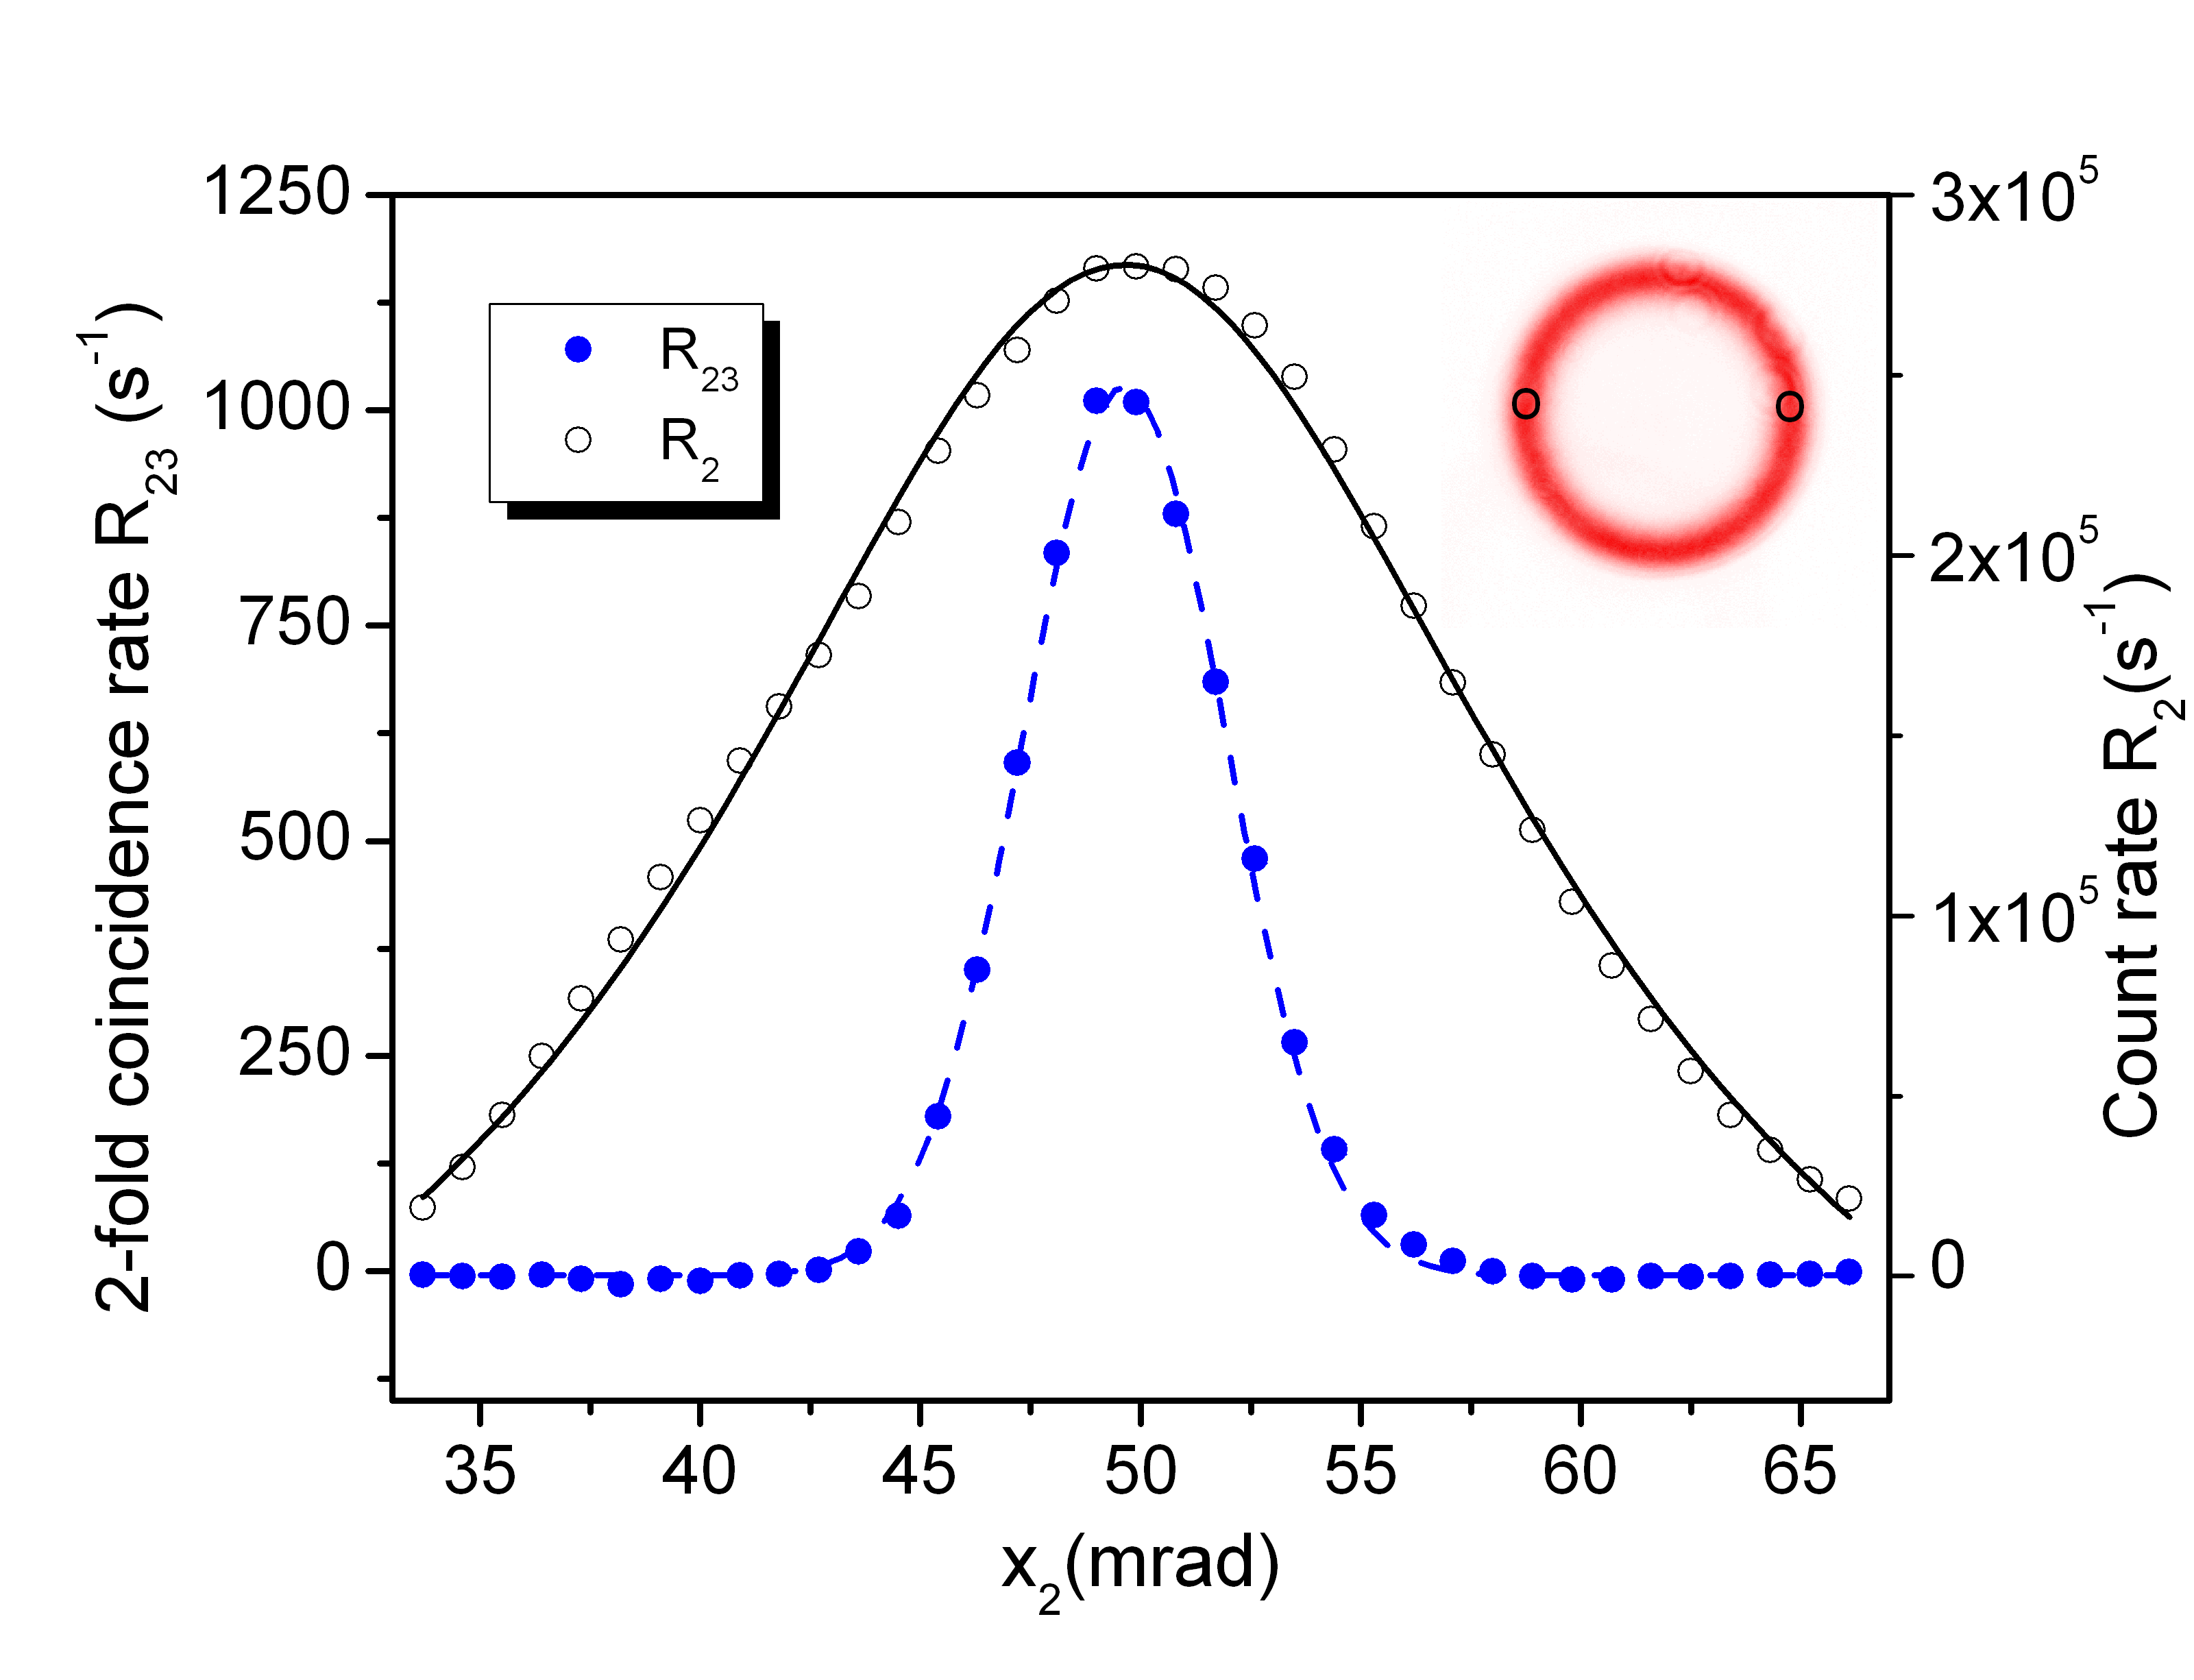
\includegraphics[width=120mm]{Fig2.png}
\caption{(Color online) Measured single count rates $R_2$ (open symbols) and 2-fold coincidence rates $R_{23}$ (filled symbols) as a function of position $x_2$, demonstrating spatial correlations in the two-photon field. The pulsed laser beam was focused in the center of the crystal using a $f$~=~250~mm lens. Data are collected using a 1 nm FWHM bandpass filter and a 1.5~mm aperture in the far-field. The solid and dashed lines indicate Lorentzian and Gaussian fits to the single and coincidence rates, respectively. The inset shows a far field image of the SPDC light emitted by the PPKTP crystal at a temperature of 20~$^\circ$C. The approximate positions of detectors D2 and D3 are shown by circles on the ring.} \label{Fig:2photons}
\end{figure}

Figure~\ref{Fig:2photons} shows the measured coincidence rate between detectors $D2$ and $D3$ (solid symbols, left axis) as a function of the position $x_2$ of detector $D_2$. Detector assembly $D_3$ is positioned at a fixed position and collects photons at an angle of -50 mrad in the far-field of the source. The measured coincidences, corrected for accidental events, are compared to the measured single count rate on detector $D2$ (open symbols, right axis). The measured single count rate on detector $D_3$ is $\sim3\cdot10^{5}$~$s^{-1}$ and is constant throughout the experiment.

The single count rate as a function of detector position is well described by a Lorentzian fit (solid line) centered at a position of 50$\pm$5~mrad and a width of 14.9$\pm$0.5~mrad FWHM. Please note that the uncertainty in the stated center position is due to the fact that it is difficult to determine the absolute position of lens $L2$ on the optical table. The characteristic minima of the $\mathrm{sinc}^2$ phase-matching curve commonly observed under continuous wave pumping are 'averaged' out by the multiple frequencies available in the spectrum of the picosecond pulsed laser~\cite{Keller1997}. The measured two-fold coincidence rate as a function of the position $x_2$ of the detector is well described by a Gaussian (dashed line) with a width (FWHM) of 5.1$\pm$0.1~mrad, and a center position of 50$\pm$5~mrad. The observation that the peak in coincidence rate is much narrower than the measured singles is a clear signature of two-photon correlations in a high-dimensional Hilbert space. The ratio of the width of the singles versus the coincidences is a direct measure of the Schmidt number $K_r$ of the (radial) spatial entanglement generated in the PPKTP crystal~\cite{DiLorenzoPires2009}. Based on the measured width of the coincidence and singles peak, we estimate a Schmidt number $K_{exp}$~$\approx$~2.9$\pm$0.1 for the pulsed laser. This estimate should be converted to a two-dimensional Schmidt number in order to compare this number to values given in literature for continuous wave pumping.

To this end, we introduce a second azimuthal Schmidt number $K_\phi$, being the ratio of the circumference of the SPDC ring, i.e. 2$\pi \times$50~mrad, over the measured width of the coincidence peak. This results in $K_\phi$~$\approx$60$\pm$6 and a corresponding Schmidt number $K$~=~$K_r K_\phi$~$\approx$~175$\pm$20. This number should be compared to calculated values~\cite{Law2004} and experimental values obtained for a 5.0~mm crystal pumped by a continuous wave laser~\cite{DiLorenzoPires2009}. The value of $K$ from ref.~\cite{DiLorenzoPires2009} for strongly negative phase mismatch (i.e. an open SPDC ring) was scaled to our case by taking into account the differences in pump beam waist and crystal length. Based on this, we expect a two-dimensional Schmidt number of $\sim$125. This value is somewhat lower than the value stated above, which we attribute to the fact that we neglected the effect of the pulsed laser on the width of the SPDC ring. The pulsed laser contains many pump frequencies which gives a slightly broader ring and consequently causes an overestimate of the value of $K_r$.

\subsection{Observation of quantum correlations of 4-photon states in the spatial degrees of freedom}

To explore the contribution of stimulated emission we measure the coincidence rate $R_{21}$ between detectors $D1$ and $D2$. Coincidences can only be registered if at least four photons are generated by a single photon pulse, since only one-photon in each pair produced by SPDC can be detected. The measured coincidence rate for photons originating from the same pulse contains both stimulated and spontaneous events. To get a measure of the number of coincidences due to spontaneous emission we introduce a tunable electronic delay between detectors $D1$ and $D2$. This allows a measurement of the coincidences in the same laser pulse ($R_{21}^{0\mathrm{ns}}$) as well as the coincidence events between subsequent laser pulses by setting the electronic delay to 12~ns ($R_{21}^{12\mathrm{ns}}$). This latter coincidence rate is dominated by events where a single pair is produced in each of the laser pulses and the coincidence rate $R_{21}^{12\mathrm{ns}}$ thus represents only the coincidence rate due to two spontaneously emitted photon pairs.

\begin{figure}[tbp]
\centering 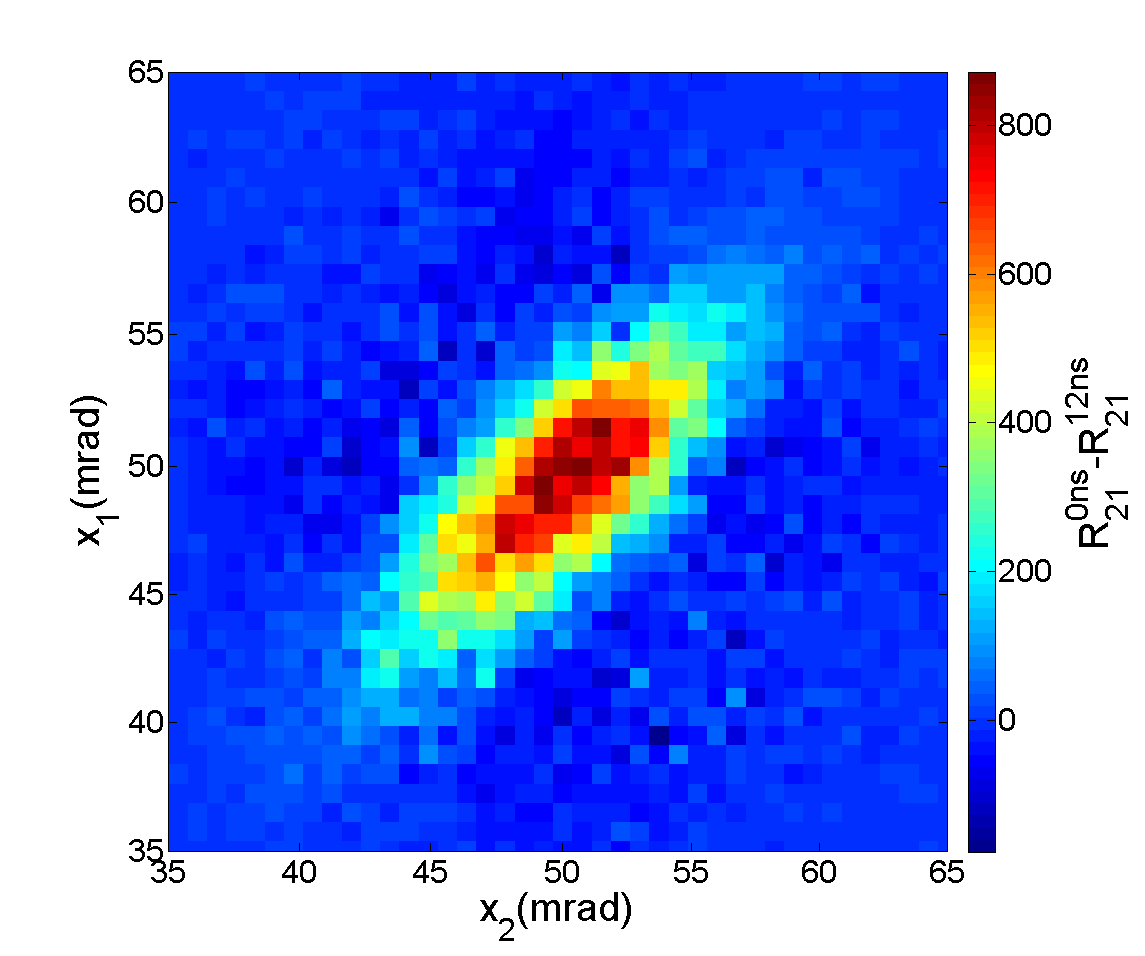
\includegraphics[width=87mm]{Fig3a.png} \\
\centering 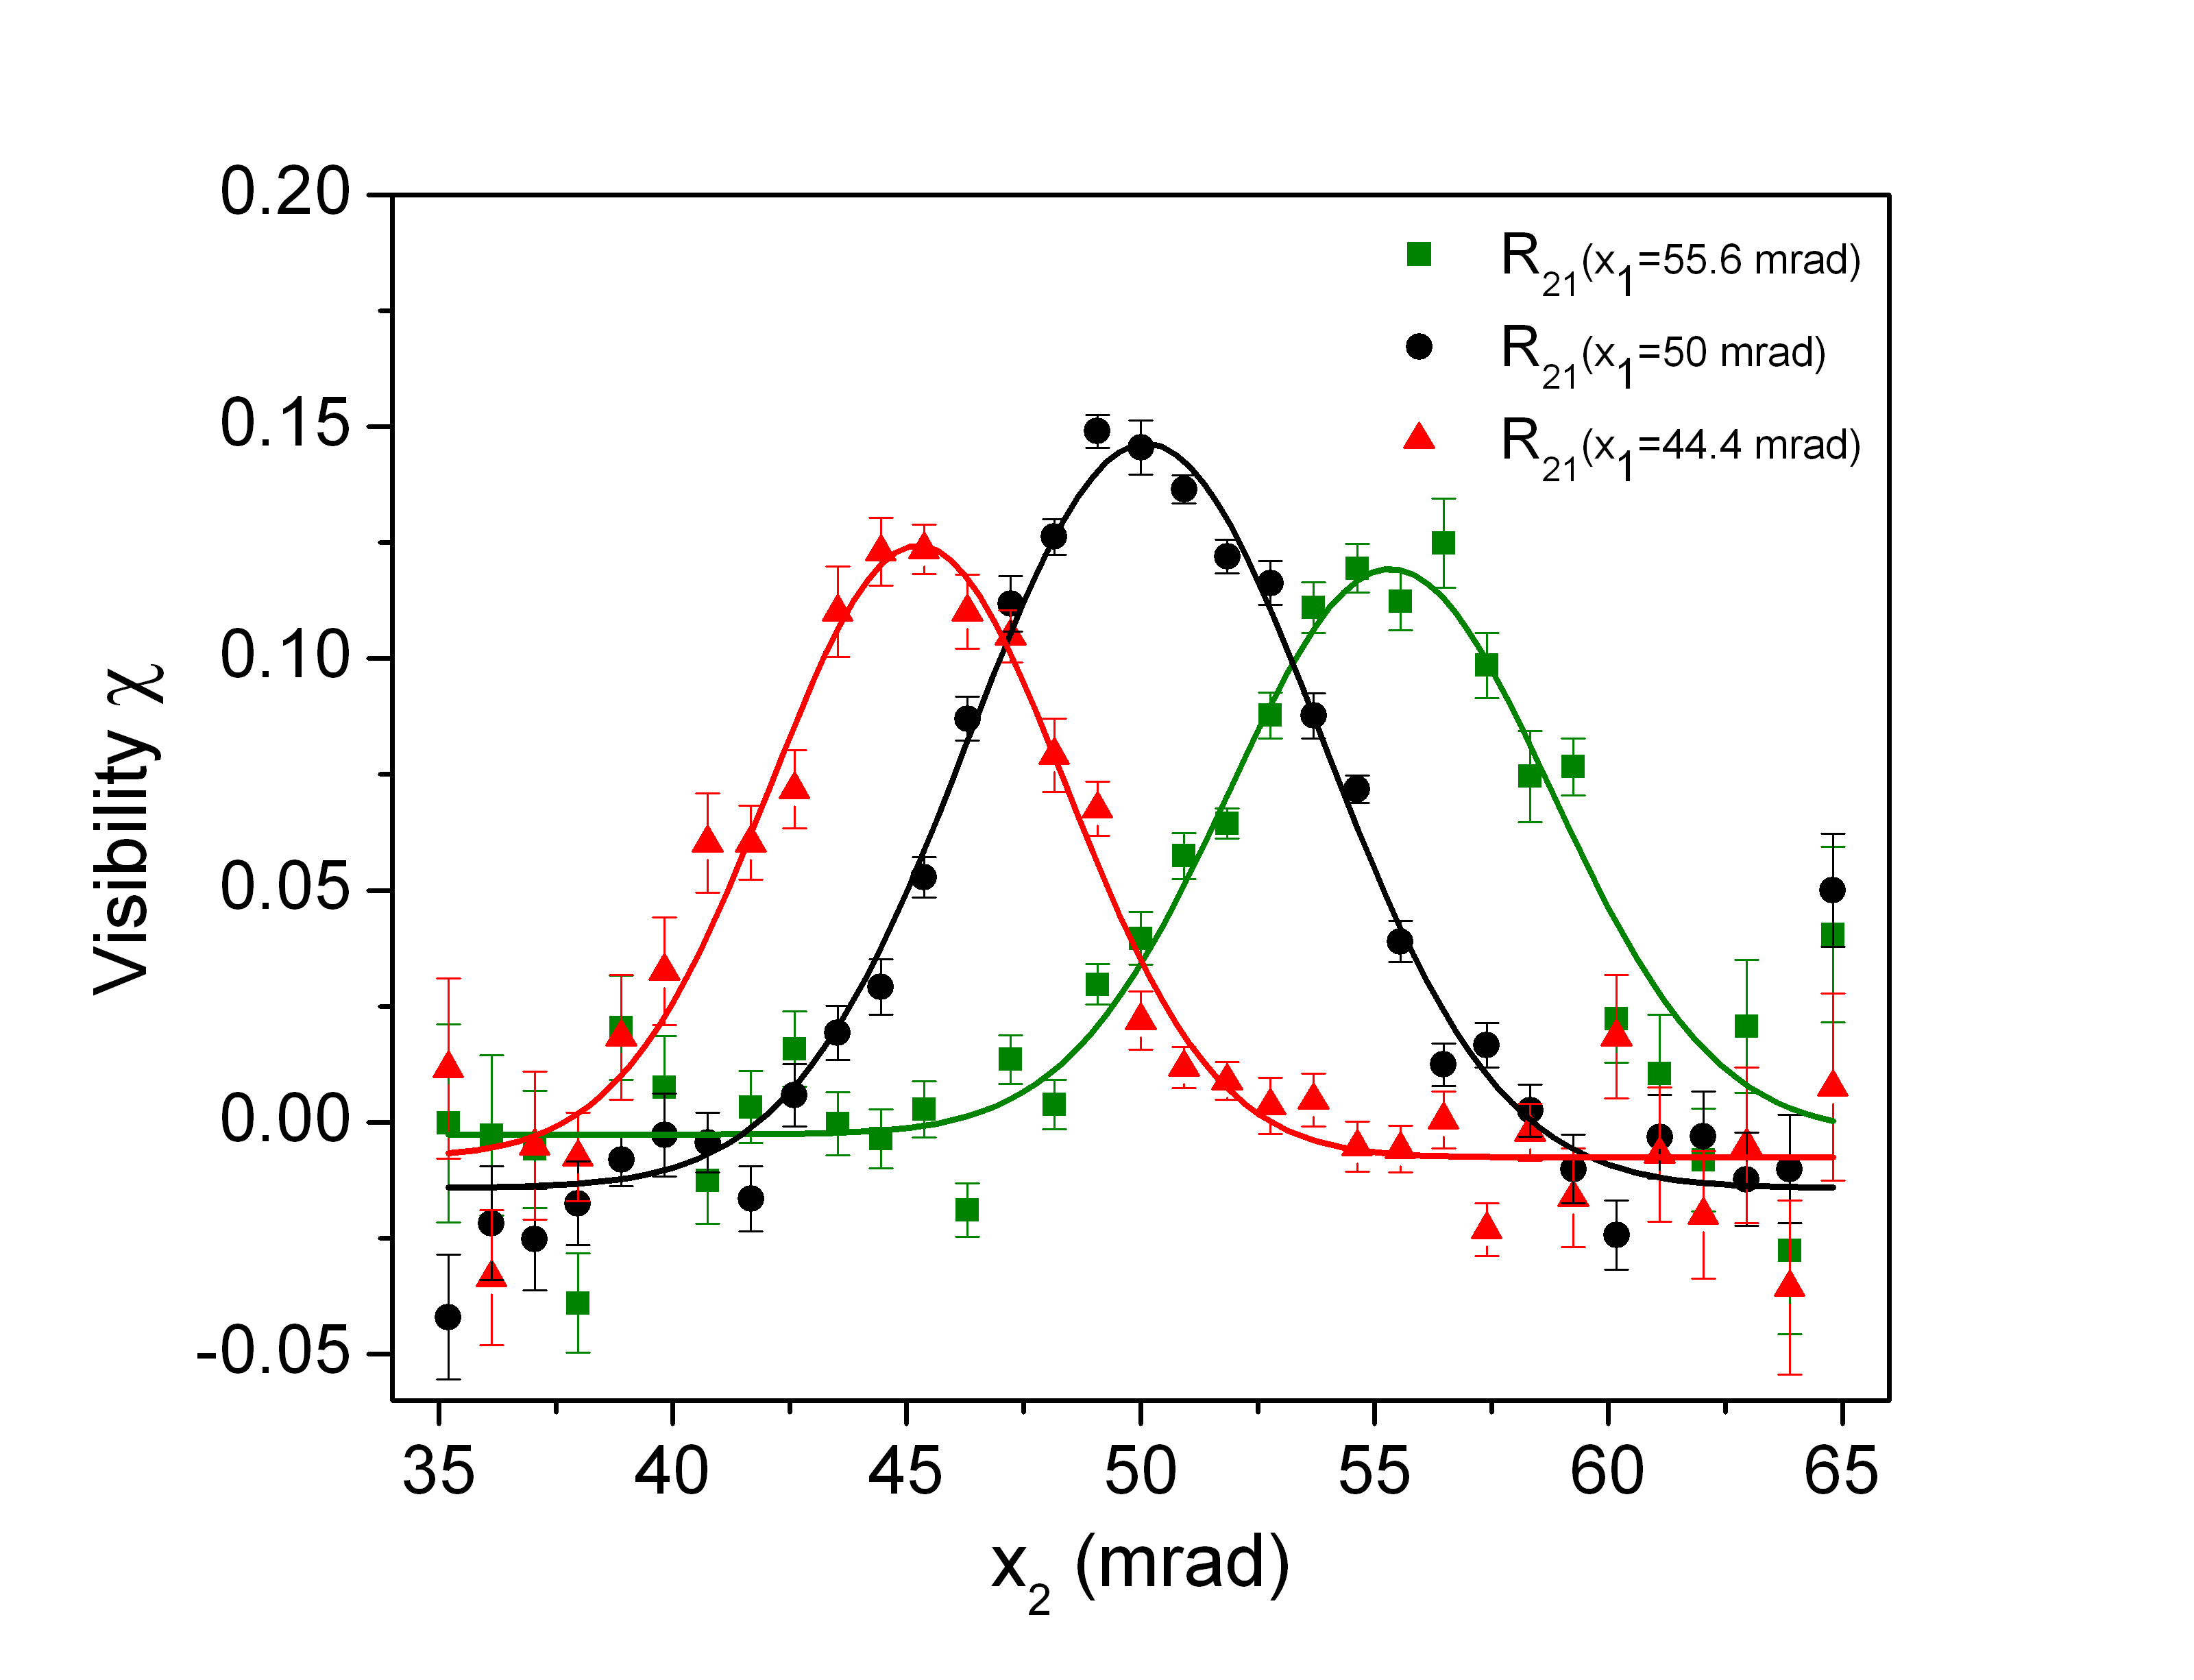
\includegraphics[width=87mm]{Fig3b.png}
\caption{(Color) Measured joint spatial distribution of stimulated pair emission. (a) False-color plot of the measured difference in coincidence rate $(R_{21}^{0\mathrm{ns}} - R_{21}^{12\mathrm{ns}})$  as a function of the positions of $x_1$ and $x_2$ of detectors $D_1$ and $D_2$. Data are collected with a 5~nm FWHM bandpass filter and a 1.5~mm aperture size. The observed maximum coincidence rate $(R_{21}^{0\mathrm{ns}}$ is typically 25,000~s$^{-1}$. The data clearly demonstrate that stimulated pair emission occurs when the photons are emitted in the same spatial mode, i.e. when $x_1$~=~$x_2$. (b) Visibility $\chi$ of the 4-photon state as a function of position $x_2$. The different symbols (triangles, circles, squares) correspond to different positions $x_1$ (44.4, 50.0, 55.6~mrad) of detector $D_1$. Data are collected using a 1~nm FWHM bandpass filter and a 1.5 mm aperture. The solid lines through the data are Gaussian fits.}\label{Fig:4photon}
\end{figure}

The difference in these coincidence rates, normalized by the coincidence rate due to spontaneous events is equal to the ``visibility'' $\chi$, i.e. $\chi = (R_{21}^{0\mathrm{ns}} - R_{21}^{12\mathrm{ns}})/R_{21}^{12\mathrm{ns}}$ and is a good measure of the extra events due to stimulated emission of 4-photon states. The measured visibility as a function of the position of the two detectors, $\chi(x_1,x_2)$, can be interpreted as a joint spatial density of stimulated pair emission. This joint spatial distribution of stimulated pair emission is depicted in Fig~\ref{Fig:4photon}. The false colour image in Fig.~\ref{Fig:4photon}a shows the difference in coincidence rate $(R_{21}^{0\mathrm{ns}} - R_{21}^{12\mathrm{ns}})$ as a function of the position $x_1$ and $x_2$ of detectors $D1$ and $D_2$ using a 5~nm bandpass filter for the SPDC light. The image is centered around the point $x_1$~=~$x_2$~=~50~mrad and clearly shows the expected positive correlation due to stimualted emission of the 4-photon state that leads to extra coincidences whenever the two detectors detect photons in the same optical mode, i.e. when $x_1$~=~$x_2$. The width (FWHM) of the peak along the diagonal ($x_1-x_2$~=~0~mrad) is 11.5$\pm$0.3 mrad, while the width along the anti-diagonal direction ($x_1+x_2$~=~100~mrad) is 4.5$\pm$0.1 mrad.

Figure~\ref{Fig:4photon}b shows the visibility $\chi(x_1,x_2)$ as a function of position $x_2$ of detector $D2$ for a fixed position of detector $D1$. The three curves correspond to $x_1$~=~44.4~mrad (triangles), 50.0~mrad (circles) and 55.6~mrad (squares). These data are taken with a 1~nm bandpass filter for the SPDC light in order to enhance the visibility at the expense of a much lower count rate. The narrow band frequency filter lowers the number of temporal modes involved, but does not affect the spatial modes. The integration time per point was increased by repeated scanning of the detector in the $x_2$ direction. Because the phase-mismatch of the PPKTP crystal that governs the SPDC process depends weakly on laser power, the long term stability of the laser becomes important. In order to correct for this effect we also monitor the single counts on the detector $D2$ as a function of position $x_2$ and exclude scans from our analysis where the SPDC ring appears shifted. The solid lines through the data are Gaussian fits to the data with a FWHM width of 8.9$\pm$0.3. The peak positions are shifted to the position of detector $D1$, such that the peak of the Gaussian appears at $x_1$~=~$x_2$. The obtained peak visibilities for the three curves are 0.13$\pm$0.01, 0.16$\pm$0.01 and 0.12$\pm$0.01. For a uniform illumination of the aperture one would expect the peak visibility to be independent of the position $x_1$. This case corresponds to a situation where the width of the SPDC ring, as given by the phase-matching function, is much larger than the shift in position $x_1$. In our experiment the slightly lower visibility for $x_1$~=~44.4 and 55.6~mrad is caused by the finite diameter of the 1.5~mm aperture that captures a non-uniform part of the SPDC ring. For larger apertures (data not shown) this decrease in visibility indeed becomes more significant.

The visibility in our experiment is limited by both the number of temporal modes collected as well as by the ratio of the total number of spatial modes available over the number of spatial modes collected by the aperture. The total number of temporal modes generated is given by the frequency bandwidth of the SPDC light as compared to the frequency spread of the pulse. For a Fourier limited pulse shape the frequency bandwidth is related to the pulse duration via $\tau = (2 \ln(2) \lambda^2)/(/\pi c \Delta \lambda)$, where $\tau$ is the pulse duration and $\lambda/\Delta \lambda$ is the relative frequency spread. The 2~ps pulse corresponds to an equivalent spectral width of 0.5~nm, while the 2~mm PPKTP crystal produces SPDC light with a bandwidth of $\sim$40 nm FWHM. Consequently, the number of available temporal modes for a PPKTP crystal pumped by a 2~ps laser is pulse is potentially $\sim$80. We use '5 nm' and '1 nm' bandpass filters centered at 826.4 nm to limit the number of temporal modes. The measured FWHM bandwidth of these filters is 4.6~nm and 1.5~nm, which extends the coherence time of the SPDC light and limit the number of temporal modes to $\sim$9 and $\sim$3 respectively. Since $\chi$ is inversely proportional to the number of available temporal modes~\cite{Riedmatten2004}, this produces upper limits to $\chi$ of 0.1 and 0.3 for the two bandpass filters. We stress that shorter pump pulses do not necessarily lead to a higher flux of photons since the phase-matching in the 2~mm PPKTP crystal effectively filters the pump pulse. In our experiments we have carefully chosen the crystal length to maximize conversion efficiency without significantly stretching the pump pulse to avoid a non-factorable structure ('X-entanglement') between spatial and temporal degrees of freedom~\cite{Gatti:PRL2009}.

\begin{figure}[tbp]
\centering 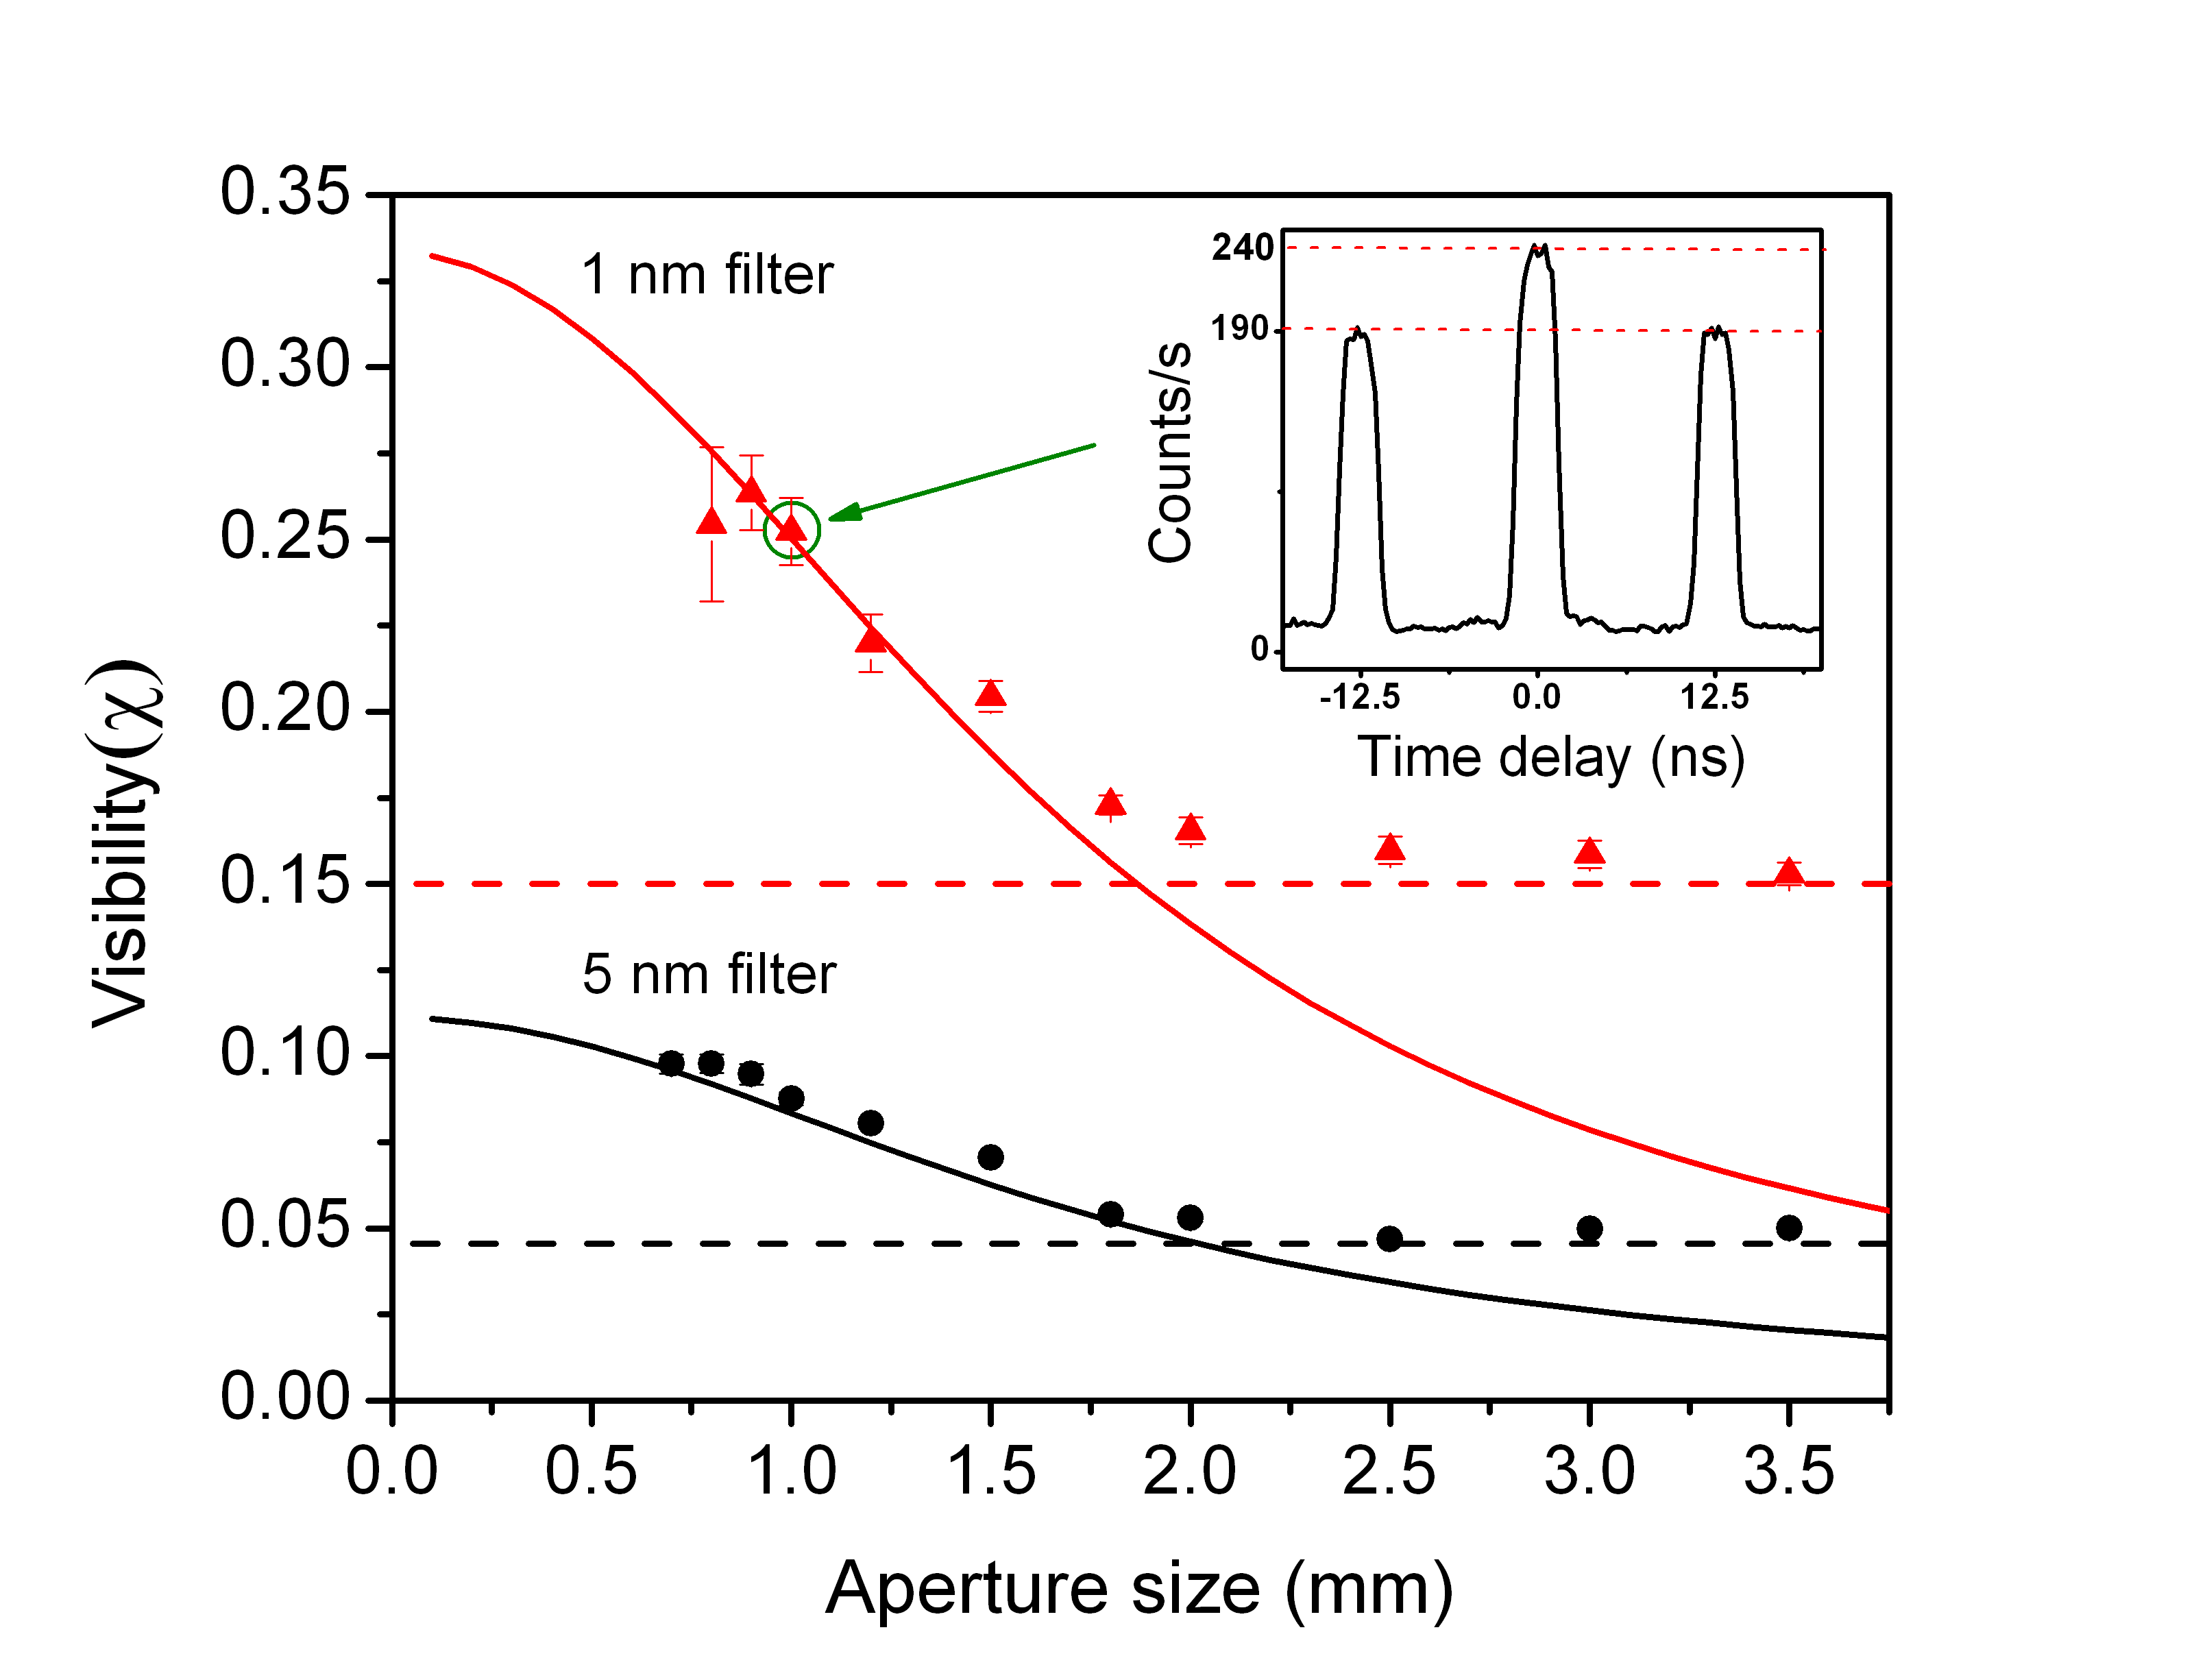
\includegraphics[width=87mm]{Fig4.png}
\caption{(Color online) Visibility $\chi$ of the 4-photon state as a function of aperture size using a 1~nm FWHM bandpass filter (triangles) and a 5~nm FWHM bandpass filter (circles). These data are obtained by subtracting the measured coincidence rate at a delay of 12~ns from the measured coincidence rate at zero delay. Typical single count rates on the detector are $1.4\times10^6$ and $3\times10^5$ sec$^{-1}$ for apertures $>$ 2 mm and drop to $5\times10^5$ and $1\times10^5$ sec$^{-1}$ for a 1 mm aperture size. The solid lines represent a calculation with no free parameters (see text). For apertures larger than 2 mm, the aperture is limited by lens $L3$ and the numerical aperture of the fiber and the visibility saturates as indicated by the horizontal dashed lines. The inset shows the measured coincidence rate $R_{12}$ as a function of electronic delay for a 1~nm FWHM bandpass filter and a 1~mm aperture size ($\chi$~=~0.25), indicated by the arrow.}\label{Fig:Visibility}
\end{figure}

Figure~\ref{Fig:Visibility} shows the measured visibility as a function of aperture size for a 5~nm bandpass filter (circles) as compared to a 1~nm bandpass filter (triangles). Measurements were performed by measuring coincidence rates between detectors $D1$ and $D2$ at a fixed position $x_1$~=~$x_2$~=~50~mrad. A measurement of the coincidence rate as a function of the electronic time delay is shown in the inset for a point with a relatively high visibility of 0.25. The extra 50 counts/sec at zero delay are due to stimulated emission of photon pairs. Clearly, the visibility is low and nearly constant for apertures that are larger than 2~mm and rises as the number of available spatial modes is reduced by closing the aperture. In our experiments the visibility saturates at apertures sizes above 2 mm where the apertures size is limited by the finite numerical aperture of the multimode fiber in combination with the focal length of the fiber coupling lens $L3$. The saturation is represented by the horizontal dashed lines.

The visibility $\chi$ in the experiment is proportional to the inverse of the number of spatial and temporal modes, i.e. $\chi \propto N_t^{-1} N_{sp}^{-1}$, where $N_t$ and $N_{sp}$ are the number of temporal and spatial modes respectively. Throughout the experiment $N_t$ is determined by the FWHM of the bandpass filter and can be considered constant. We use values of $N_t$ = 9 and $N_t$ = 3 for the two different bandpass filters. In order to estimate the number of spatial modes collected as a function of aperture size we consider the correlations between two point-like apertures at positions $\vec{r_1}$ and $\vec{r_2}$. The resulting visibility is given by:
\begin{equation}
\chi(\vec{r_1},\vec{r_2})=\exp(-\frac{|\vec{r_1}-\vec{r_2}|^2}{r_0^2}).
\end{equation}
The characteristic distance $r_0 = (\lambda f_2)/(\pi w_p)$, where $f_2$ = 270 mm is the focal distance of lens $L2$ that creates the far-field of the SPDC source and $w_p$ is the waist of the pump beam created by focussing the pump beam using lens $L1$. Using the measured waist of the pump beam of 80~$\mu$m we find a characteristic distance $r_0$~=~0.9 mm. The visibility in the experiment due to finite aperture size for two apertures centered at the same position can be found via integration:
\begin{equation}
 \chi (a) = \frac {1}{N_t \pi^2 a^4} \iint \chi(\vec{r_1},\vec{r_2}) \Theta(|\vec{r_1}|-a) \Theta(|\vec{r_2}|-a) \mathrm{d}\vec{r_1} \mathrm{d}\vec{r_2}, \label{vis}
\end{equation}
where the Heaviside step-functions $\Theta(|\vec{r_1}|-a)$ and $\Theta(|\vec{r_2}|-a)$ represent the sharp edges of the two apertures with equal radius $a$ in the far-field. The solid lines through the data in Fig.~\ref{Fig:Visibility} are the results of calculating the double integral represented by equation~\ref{vis} using 3 and 9 temporal modes for the two bandpass filters and the calculated value of $r_0$ based on the measured beam waist. The agreement between the data and the model with no adjustable parameters is striking for aperture sizes below 2 mm. For apertures above 2 mm the visibility saturates, as indicated by the horizontal dashed lines, at a value determined by lens $L3$ and the numerical aperture of the multimode fiber that limit the beam diameter to $\sim$2~mm.

\section{Conclusion}

In conclusion, we have demonstrated the existence of spatial correlations between photon pairs in a 4-photon state. These correlations are induced via stimulated pair emission. In our experiments we are able to separate the contribution from spontaneous parametric down-conversion and stimulated parametric down-conversion at the level of double pairs. The stimulated emission becomes important when a 2~mm long PPKTP crystal is pumped by a 2~ps pulsed laser at 413.2~nm wavelength to create frequency and polarization degenerate photon pairs at a wavelength of 826.4~nm. The spatial correlations of the stimulated photon pairs contains a rich structure when using a non-colinear geometry for the down-conversion process, which can be explored with relative ease using apertures in the far-field. In this way we present the first measurements of the joint spatial distribution of stimulated pair emission and discuss the acquired visibility. This technique opens new possibilities to explore the structure of higher-dimensional entanglement by making use of spatial degrees of freedom instead of the temporal degree of freedom. The possibility to distinguish between stimulated and spontaneous processes can be used to explore recent proposals for ghost imaging with thermal and quantum light sources\cite{Chan:PRA2009,Osullivan:PRA2010}.



%\appendix
%\include{appa}

\section*{Acknowledgements}
This research was made possible by financial support from the Dutch Association for Scientific Research (NWO) and the Foundation for Fundamental Research of Matter (FOM).

%\nocite{Brandt2013}*}
\bibliographystyle{lion-msc}
\bibliography{BRP}

\clearpage
\subsection*{Reference star differential imaging}
Reference star differential imaging (RDI) is a calibration technique that uses the point spread function (PSF) of a similar star as the observed object, without a disk. The PSF from the hosting star is static, so if this could be subtracted, the contrast between the star and the disk is much bigger. It is hard to find a reference star that has been observed in the same mode, in the same period and with the same conditions. All these things can change the PSF drastically, which means that it is impossible to subtract the PSF of reference star. The reference star also has to have about the same spectrum, in order to deal properly with the luminosity difference in different wavelength bins of the different spectral types and the fact that the IFS takes data over a range of wavelengths. 
\bigskip

The distorted wavefront that has to be corrected by the adaptive optics of the VLT is measured in the R-band filter. De extreme adaptive optics of the VLT is very sensible and slightly magnitude dependend, which just means that the adaptive otics work better if a brighter object is observed. Consequence of this, is that the reference star to apply RDI, has to be the same order of magnitude in the R band as the observed object. A different performance of the adaptive optics, can change the PSF such that it is not suitable for reference star subtraction anymore. 

\end{document}

